\documentclass[usenatbib,fleqn]{mn2e}

\makeatletter
\newlength{\abovecaptionskip}%
\setlength{\abovecaptionskip}{10\p@}
\makeatother
\usepackage{threeparttable}


\usepackage{amsmath,amssymb}
\usepackage{mathrsfs}
\usepackage{graphicx}
\usepackage{epstopdf}
\usepackage{hyperref}
\epstopdfsetup{outdir=./figures/}
\graphicspath{{./figures/}}
\usepackage{url}
\usepackage{aas_macros}
\usepackage{astro}
\usepackage{deluxetable}
% \usepackage{natbib}

% \renewcommand{\l}{\left}
% \renewcommand{\r}{\right}

\newcommand{\Mdot}{\dot{M}}
\newcommand{\eddr}{\dot{M}/\dot{M}_{\rm Edd}}
\newcommand{\MdotEdd}{\dot{M}_{\rm Edd}}
\newcommand{\Mdotb}{\dot{M}_{\rm bondi}}

\newcommand\lsim{\mathrel{\rlap{\lower4pt\hbox{\hskip1pt$\sim$}}
    \raise1pt\hbox{$<$}}}
\newcommand\gsim{\mathrel{\rlap{\lower4pt\hbox{\hskip1pt$\sim$}}
    \raise1pt\hbox{$>$}}}
\newcommand{\rs}{r_s}
\newcommand{\rb}{r_b}
\newcommand{\rcirc}{r_{\rm circ}}
\newcommand{\rss}{r_{\rm ss}}
\newcommand{\lrs}{\l_{\rs}}
\newcommand{\lambdars}{\lambda_{\rs}}
\newcommand{\vw}{\tilde{v}_{w}}

\newcommand{\dxdy}[2]{\frac{d #1}{d #2} }
\newcommand{\ddr}[1]{\dxdy{#1}{r}}
\newcommand{\drhodt}{\dxdy{\rho}{t}}
\newcommand{\dpdr}{\dxdy{p}{r}}
\newcommand{\dvdr}{\dxdy{v}{r}}
\newcommand{\dsdr}{\dxdy{s}{r}}
\newcommand{\dphidr}{\dxdy{\Phi}{r}}

\newcommand{\ke}{\frac{v^2}{2}}
\newcommand{\kew}{\frac{\tilde{v}_{w}^2}{2}}

\newcommand{\gammaf}{\frac{\gamma}{\gamma-1}}
\newcommand{\gammafi}{\frac{\gamma-1}{\gamma}}
\newcommand{\cs}{\frac{p}{\rho}}
\newcommand{\Q}{q (\ke+\kew-\gammaf \cs)}

\newcommand{\kb}{k_{\rm b}}
\renewcommand{\mp}{m_{\rm p}}
\newcommand{\pc}{\rm pc}

\newcommand{\Menc}{M_{\rm enc}}
\newcommand{\rhostar}{\rho_*}
\newcommand{\Mstar}{M_{\star}}
\newcommand{\Mseight}{M_{\star,8}}
\newcommand{\Mbh}[1][]{M_{\bullet#1}}
\newcommand{\Mbheight}{M_{\bullet,8}}
\newcommand{\MbheightExp}{\frac{\Mbh}{10^8 \Msun}}

\newcommand{\phirs}{\frac{G \Menc}{\rs}}
\newcommand{\soi}{\rm soi}
\newcommand{\rsoi}{r_{\soi}}
\newcommand{\rIa}{r_{\rm Ia}}
\newcommand{\EIa}{E_{\rm Ia}}
\newcommand{\RateIa}{R_{\rm Ia}}
\newcommand{\sigsoi}{\sigma_{\soi}}

\newcommand{\vwO}{v_{w}}
\newcommand{\kewO}{\frac{\vwO^2}{2}}
\newcommand{\x}{\frac{r_s}{\rsoi}}
\newcommand{\vwNorm}{\frac{\vwO}{\sigsoi}}
\newcommand{\vwOFH}{v_{500}}
\newcommand{\vwOFHexp}{\frac{\vwO}{500 \, {\rm km/s}}}

\newcommand{\pyear}{{\rm yr}^{-1}}
\newcommand{\tage}{t_{\star}}
\renewcommand{\th}{t_h}
\newcommand{\tcool}{t_{\rm cool}}
\newcommand{\tff}{t_{\rm ff}}

\topmargin -1 cm

\author[Generozov, Stone, \& Metzger]{Aleksey Generozov$\thanks{E-mail: ag@astro.columbia.edu}$, Nicholas Stone, Brian~D.~Metzger\\
  Columbia Astropysics Labratory, Columbia University, 550 West 120th Street, New York, NY 10027}


\begin{document}
\title{Circumnuclear Media and Accretion Rates of Quiescent Supermassive Black Holes}
\maketitle

\begin{abstract}
We calculate steady-state, one-dimensional hydrodynamic profiles of hot gas in the nuclei of nominally quiescent galaxies for a range of central black hole mass $M_{\bullet}$, parameterized gas heating rate, and observationally-motivated stellar density profiles.  Mass is supplied to the circumnuclear medium by stellar winds, while gas is heated primarily by stellar winds, supernovae, and black hole feedback.  Analytic estimates are provided for the stagnation radius (where the radial velocity of the gas passes through zero) and the black hole mass accretion rate, $\dot{M}$, as a function of black hole mass and the gas heating efficiency, the latter of which is related to the star-formation history.  We assess the conditions under which radiative instabilities develop, separately in the case of a single burst of star formation and in the case of the average star formation history of galaxies hosting a given black hole mass. The nuclear X-ray luminosities of a sample of quiescent black holes are combined with our results for $\dot{M}$ and an estimate of the radiative efficiency of the accretion flow to conclude that quiescent black holes in the local universe are consistent with accreting in a locally thermally-stable state.  The maximum accretion rate of a thermally-stable flow is, however, too low to explain the accretion rates and short growth time of low mass black holes in the local universe.  The latter must instead result from gas being fed in from large radii, either due to galaxy mergers associated with hierarchical growth or thermal instabilities on larger (galactic) scales.  We briefly discuss implications of our results for the use of an assumed $\dot{M}-M_{\bullet}$ relationship to constrain the occupation fraction of SMBHs in low mass galaxies and the diversity of circumnuclear environments encountered by the jetted outflows from tidal disruption events.
\end{abstract}

\begin{keywords}
  black hole physics --  galaxies: active
\end{keywords}


\section{Introduction}
\label{sec:introduction}

Supermassive black holes (SMBHs) lurk in the centers of most, if not
all nearby galaxies (see reviews by,
e.g. \citealt{KormendyRichstone:1995a};
\citealt{FerrareseFord:2005a}). However, only a few percent of these
manifest themselves as luminous Active Galactic Nuclei (AGN).  Nearly
quiescent SMBHs, such as those hosting low luminosity AGN, constitute
a silent majority (e.g.~\citealt{Ho:2009a}).

Understanding why most SMBHs appear to be inactive requires
characterizing their gaseous environments.  Gas near the sphere of
influence of the SMBH, hereafter the `circumnuclear medium' (CNM),
controls the mass accretion rate, $\dot{M}$.  The accretion rate in
turn sets the luminosity of the black hole and the impact of this
energy and momentum output on larger physical scales (`feedback').
The presence of dense gas in the nucleus may also lead to runaway
cooling, resulting in bursty episodes of star formation and AGN
activity (e.g.~\citealt{Ciotti&Ostriker07}; \citealt{Ciotti+10}).

Knowledge of how $\dot{M}$ depends on the SMBH mass, $\Mbh$, and other
properties of the galactic nucleus informs key questions related to
the co-evolution of SMBHs and their host galaxies with cosmic time
(e.g.~\citealt{Kormendy&Ho13}; \citealt{Heckman&Best14}).  SMBH growth
in the low redshift universe is dominated by low mass black holes,
$M_{\bullet} \lesssim 10^{8}M_{\odot}$ (e.g.~\citealt{Heckman+04}), a
fact which is often attributed to the general trend of `cosmic
down-sizing' resulting from hierarchical structure growth (e.g,
\citealt{Gallo+08}).  However, the physical processes involved in the
growth of low mass blacks may be distinct from those operating at
higher SMBH masses and accretion rates in quasars.  A key question
here is whether SMBHs grow primarily by accreting gas fed in directly
from large scales, or whether significant growth results also from
internal, secular processes such as local stellar mass loss.

Obtaining a better undersatnding of the physical mechanisms
responsible for accretion onto quiescent SMBHs would have implications
for observational constraints on the occupation fraction of SMBHs in
low mass galaxies, and the potential existence of intermediate mass
black holes.  \citet{Miller+15} combine the average correlation
between $\Mbh$ and the nuclear X-ray luminosities, $L_{X}$ of a sample
of elliptical galaxies to infer tentative evidence for a SMBH
occupation fraction less than unity in galaxies with stellar masses
$M_{\star} \lesssim 10^{10}M_{\odot}$ ($M_{\bullet} \lesssim
10^{7}M_{\odot}$).  This method relies on extrapolating a power-law
fit of the $L_X-\Mbh$ distribution to low values of $L_{\rm X}$ below
the detection threshold, despite the potential that rather different
physical processes control the accretion rates onto the lowest mass
SMBHs.

%The conclusions of
%\citet{Miller+15} are thus sensitive to possible changes in
%the $L_X$-$\Mbh$ relationship at small $\Mbh$.
% AG: In our model we obtain a steeper relationship, but we have difficulty matching the observed relationship above the detection threshold

The CNM density also influences the emission from stellar tidal
disruption events (TDEs), such as the high energy transient {\it
  Swift} J1644+57 (\citealt{Levan+11}; \citealt{Bloom+11},
\citealt{Burrows+11}; \citealt{Zauderer+11}).  This event was powered
by a transient relativistic jet, which produced synchrotron radio
emission as the jet material was decelerated by shock interaction with
the CNM of the previously quiescent SMBH
(\citealt{Giannios&Metzger11}; \citealt{Zauderer+11}).  Detailed
modeling of J1644+57 showed that the CNM density was significantly
lower than that measured surrounding Sgr A$^{\star}$
(\citealt{Metzger+12}; \citealt{Berger+12}).  However, a TDE jet
injected into a denser CNM would be decelerated more rapidly,
producing substantially different radio emission than in J1644+57.
Variations in the properties of the CNM could thus in principle help
explain why most TDEs appear to be radio quiet
(e.g.~\citealt{Bower+13}; \citealt{VanVelzen+13}).

Gas comprising the CNM can in principle originate from several
sources: (1) wind mass loss from predominantly evolved stars; (2)
stellar binary collisions; and (3) unbound debris from a recent TDE.
Stellar wind mass loss is probably the dominant source insofar as
collisions are relevant only in extremely dense stellar environments
for very young stellar populations (\citealt{Rubin&Loeb11}), while
\citet{MacLeod+13} find that TDEs contribute subdominantly to the
time-averaged accretion rate of quiescent SMBHs.

\citet{Ho:2009a} estimates the accretion rates onto a sample of
early-type galaxies both by using X-ray observations to determine the
Bondi accretion rate and using estimates for the mass loss rate of
evolved stars.  Both methods lead to the conclusion that the available
gas reservoir is more than sufficient to power the observed
low-luminosity AGN, assuming the standard $\sim$ 10 per cent radiative
efficiency for thin disk accretion.  Several independent strains of
evidence now suggest that low-luminosity AGN result from accretion
proceeding in a radiatively inefficient mode
(\citealt{Yuan&Narayan14}), due either to the advection of
gravitationally-released energy across the SMBH horizon
(e.g.~\citealt{Narayan&Yi95}) or due to a low efficiency for the gas
inflowing on large scales ultimately reaching the SMBH
(e.g.~\citealt{Blandford&Begelman99}; \citealt{Li+13}).

%In fact, the temperature profile is assumed to be flat inside of the
%Bondi radius.  In reality, the cusp in the velocity dispersion near
%the SMBH, should cause a cusp in the gas temperature profile (assuming
%the kinetic energy of stellar winds is efficiently thermalized in
%shocks).
%% AG-give sense of scale.

Another approach to determine the SMBH accretion rate, which we adopt
in this paper, is to directly calculate the density, velocity and
temperature profiles of the CNM using a physically motivated
hydrodynamic model.  Mass is injected to the nuclear environment via
stellar winds, while energy input results from several sources
including stellar winds, supernovae, and AGN feedback
(\citealt{Quataert:2004a,De-ColleGuillochon+:2012a,ShcherbakovWong+:2014a}).
Unlike previous works focusing on modeling individual galaxies, here
we systematically analyze the properties of the CNM across a sample of
galaxies with a range of SMBH masses, stellar density profiles, and
star formation histories (\citealt{WangMerritt:2004a}).

Past studies, employing multi-dimensional numerical hydrodynamics and
including variety of (parameterized) physical effects, have focused on
massive elliptical galaxies (e.g.~\citealt{Ciotti&Ostriker07};
\citealt{Ciotti+10}).  A key finding of these works is the periodic
development of cooling instabilities, which temporarily increase the
gas accretion rate until black hole feedback becomes sufficiently
important to shut off the flow and halt SMBH growth.  Here we instead
focus on time-independent models, neglecting radiative cooling.  This
approach allows us to systematically explore the relevant parameter
space and to derive simple analytic expressions that prove useful in
exploring whether cooling instabilties manifest across the expected
range of galaxy properties, or whether other (non-AGN) forms of
feedback can result in steady accretion.  Even if cooling instabilties
develop on galactic scales over longer timescales, e.g. $\sim$ Gyr, a
state of quasi-steady accretion may exist between these inflow events
on smaller radial scales comparable to the sphere of influence.  We
are thus motivated to explore whether steady flow is achieved within
the nucleus under any circumstances, or whether the gas content is
always building towards instability.
%A chief goal of our analysis is to provide a framework for interpreting the properties of quiescent galactic nuclei given the comparatively well understood physics of stellar winds and supernova heating.

In the presence of strong heating, one-dimensional steady-state flow
is characterized by an inflow-outflow structure, with a critical
radius known as the``stagnation radius" $\rs$ where the radial
velocity passes through zero.  Mass loss from stars interior to the
stagnation radius is accreted, while that outside $\rs$ is unbound in
an outflow from the nucleus.  The stagnation radius, rather than the
Bondi radius, thus controls the SMBH accretion rate (although we will
show that $\rs$ can in many cases lie within a factor of few of the
nominal Bondi radius).  In the case of sufficiently weak heating,
however, no stagnation radius may exist at all, i.e. the entire ISM of
the galaxy is feeding the SMBH.  Another goal of this work is to
assess under what conditions a stagnation radius exists, as this
question is intimately tied to that of cooling instability.
% Furthermore, in some cases we find that no stagnation
% radius exists at all; this formally implies that the entire of ISM of
% the galaxy is feeding the SMBH, potentially resulting in much higher
% accretion rate than would be predicted by simple Bondi accretion. 


This paper is organized as followed.  In $\S\ref{sec:model}$ we
describe our model, including the sample of galaxies used in our
analysis ($\S\ref{sec:gal_model}$) and our numerical procedure for
calculating the steady-state hydrodynamic profile of the CNM
($\S\ref{sec:hydro}$).  In $\S\ref{sec:results}$ we describe our
results.  In $\S\ref{sec:applications}$ we describe applicaiton of our
results, including a comparison of our gas profiles to those inferred
from {\it Chandra} observations and to the measured $L_X-\Mbh$
relationship.  In $\S\ref{sec:discussion}$ we discuss our results.  In
$\S\ref{sec:summary}$ we summarize our results.  Table \ref{table:definitions} provides the definitions of commonly used variables.


\begin{table*}
\begin{threeparttable}
%\centering
\begin{minipage}{18cm}
\caption{Definitions of commonly used variables}
\begin{tabular}{lc}
\hline
{Variable} & {Definition} \\
\hline
$M_{\bullet}$ & Black hole mass \\
$\tilde{v}_{w}$ & Total heating parameter, including minimum heating rate from stellar velocity dispersion \\
$v_{w}$ & Total heating parameter, excluding heating rate from stellar velocity dispersion \\
$r_{s}$ & Stagnation radius (where radial velocity goes to zero) \\
$r_{\rm soi}$ & radius of sphere of influence (eq.~[\ref{eq:rsoi}]) \\
$r_{\rm b}$ & outer break radius of stellar density profile \\  
\hline
\label{table:definitions}  
\end{tabular}
\begin{tablenotes}
\item{$^{(a)}FILL IN$}
\end{tablenotes}
\end{minipage}
\end{threeparttable}

\end{table*}


\section{Model}
\label{sec:model}
\subsection{Galaxy models}
\label{sec:gal_model}
\citet{LauerFaber+:2007a} use Hubble Space Telescope WFPC2 imaging to measure the radial surface brightness profiles for hundreds of nearby early type galaxies. The measured brightness profile is generally well-fit by a ``Nuker" law parameterization:
\begin{equation}
  I(\xi)=I_b 2^{(\beta-\Gamma)/\alpha} \xi^{-\Gamma} (1+\xi^\alpha)^{-(\beta-\Gamma)/\alpha}, \,\,\,\xi\equiv\frac{r}{r_b},
\end{equation}
i.e., a broken power law that transitions from an inner power law slope, $\Gamma$, to an outer power law slope, $\beta > \Gamma$, at a break radius, $\rb$.  Assuming the stellar population is spherically symmetric, this corresponds to a stellar density $\rhostar \propto r^{-1-\Gamma}$ for $r \ll \rb$ and $\rhostar\propto r^{-1-\beta}$ for $r \gg \rb$.  To good approximation
\begin{align}
\rho_\star = 
\begin{cases}
\rho_\star(\rsoi) \left(r/\rsoi\right)^{-1-\Gamma} & r \leq r_b\\
\rho_\star(r_b) \left(r/r_b\right)^{-1-\beta} & r > r_b,
\label{eq:rhostar}
\end{cases}
\end{align}
where $\rho_\star(\rsoi)$ is the stellar density at the radius of the black hole sphere of influence (soi), 
\be
\rsoi \simeq G \Mbh/\sigma^2 \approx 14 M_{\bullet,8}^{0.6}\,{\rm pc},
\label{eq:rsoi}
\ee
where $M_{\bullet,8} \equiv M_{\bullet}/10^{8}M_{\odot}$ and the second equality in (\ref{eq:rsoi}) employs the $\Mbh-\sigma$ relationship of \citet{Gultekin+09},
 \begin{align}
M_{\bullet} \simeq 2\times 10^{8}\left(\frac{\sigma}{200\,{\rm
      km\,s^{-1}}}\right)^{5.1}M_{\odot}.
\label{eq:Msigma}
\end{align}
The use of equation (\ref{eq:Msigma}) is questionable for low mass black holes (e.g., \citealt{Greene&Ho07}), but our results are not overly sensitive to this assumption.  

A galaxy model is fully specified by four parameters: $\Mbh$,
$\Gamma$, $r_b$, and $\beta$.  We compute models for three different
black hole masses, $\Mbh = 10^6$, $10^7$, $10^8 \Msun$.  The
distribution of $\Gamma$ in the \citet{LauerFaber+:2007a} sample is
bimodal, with a concentration of ``core" galaxies with $\Gamma \lsim
0.3$ and a concentration of ``cusp" galaxies with $\Gamma \gsim 0.7$.
We bracket these possibilities by considering models with $\Gamma=0.8$
and $\Gamma=0.1$.  

We fix $\beta = 2$ (a typical value) because our results are generally not sensitive to the
properties of the gas flow on radial scales $\gtrsim r_b$. The presence of the break radius $r_{b}$ is, however, necessary to obtain a converged steady state for some regions of our parameter space.  We consider solutions calculated for up to four values of $\rb$: 50 pc, 100 pc, 200 pc, and 400 pc, motivated by the range of break radii from the \citet{LauerFaber+:2007a} sample.\footnote{For the core galaxies the break radius follows the scaling relationship $\rb\sim 106 \, (\Mbheight)^{0.39}$ pc, with scatter of approximately one dex.  Most the cusp galaxies have
$\rb$ between 100 and 1000 pc, without a clear trend with $\Mbh$.}  In practice we calculate solutions for a range of $\rb$ only in cases when its precise value is expected to have a significant affect on the solution, in particular for high SMBH masses and low heating rates, for which the stagnation radius approaches large radii.   


\subsection{Hydrodynamic Equations}
\label{sec:hydro}

Following \citet{Quataert:2004a} (see also \citealt{HolzerAxford:1970a,De-ColleGuillochon+:2012a,ShcherbakovWong+:2014a}), we calculate the density $\rho$, temperature $T$, and radial velocity $v$ of the CNM for each galaxy model by solving the equations of one-dimensional, time-dependent hydrodynamics,
\begin{align}
  &\drhodt+\frac{1}{r^2}\frac{\partial}{\partial r}\left(\rho r^2 v\right)=q \label{eq:drhodt}\\
  &\rho \left(\frac{\partial v}{\partial t} + v\frac{\partial
      v}{\partial r}\right) =-\frac{\partial p}{\partial r}- \rho\frac{GM_{\rm enc}}{r^{2}} -q v \label{eq:dvdt}\\
  &\rho T\left(\frac{\partial s}{\partial t} + v\frac{\partial
      s}{\partial r}\right)=q\left[\ke+\kew-\gammaf \cs \right] 
, 
\label{eq:dsdt}
\end{align}
where $p$ and $s$ are the pressure and specific entropy, respectively, and $M_{\rm enc} = M_{\star}(r) + \Mbh$ is the
enclosed mass.  We adopt an ideal gas equation of state with $p = \rho kT/\mu m_p$ with $\mu = 0.62$  and $\gamma = 5/3$. 

The source term in equation (\ref{eq:drhodt}),
\begin{align}
  q=\frac{\eta \rhostar}{\th},
\label{eq:q}
\end{align}
represents mass input from stellar winds, which we parameterize in
terms of the fraction $\eta$ of the stellar density $\rhostar$ being
recycled into gas on the Hubble time $\th = 1.4 \times 10^{10}$
yr.  To good approximation $\eta\simeq 0.02 (\tau_{\star}/t_h)^{-1.3}$ at time $\tau_{\star}$ following an impulsive star burst (e.g., \citealt{Ciotti+91})\footnote{\citet{Ciotti+91} give the mass return rate from evolved stars as a function of B-band luminosity instead of volumetrically, but our expressions are equivalent.}, although $\eta$ is significantly higher for continuous star formation histories (Fig.~\ref{fig:eta}).  

Source terms $\propto q$ also appear in the momentum and entropy
equations (eqs.~[\ref{eq:dvdt}] and [\ref{eq:dsdt}]) because the isotropic injection of mass represents, in the SMBH rest frame, a source of momentum
and energy relative to the mean flow.  Physically, these result from
the mismatch between the properties of virialized gas injected locally
by stellar winds and the mean properties of the background flow.  The
term $\propto -q c_{s}^{2}$ is important because it acts to potentially stabilize the flow to runaway cooling ($\S\ref{sec:instability}$).

The term $\propto \vw^2 = \sigma(r)^2+v_{w}^2$ in the entropy
equation accounts for external heating sources (e.g.,
\citealt{ShcherbakovWong+:2014a}).  The first term approximates the
minimum amount of shock heating from stellar winds due to the random movement
of stars with respect to one another at the characteristic velocity of $\sigma \approx \sqrt{GM_{\rm enc}/r}$.  This heating is present even in old stellar populations for which mass and energy injection are dominated by AGB winds with low velocities $\ll \sigma$.  The second term, $v_{w}^{2}$, parameterizes all additional sources of heating, including faster main
sequence or Wolf-Rayet stellar winds, spin-down energy from millisecond pulsars, supernovae, AGN
feedback, etc.  As will be discussed in $\S\ref{sec:heating}$, the value of
$v_{w}$ will in general depend on the SMBH mass and
the age of the stellar population.  We further assume that $v_w$ is constant with radius, i.e. that the volumetric heating rate is proportional to the local stellar density.

To isolate the physics of interest, our baseline calculations neglects three potentially important effects: heat conduction, radiative cooling, and rotation.  Our justification for neglecting rotation will be discussed further in $\S\ref{sec:rotation}$.  Electron heat conduction results in an an additional term on the right hand side of the entropy equation of the form:  
\be \dot{q}_{\rm cond} = \nabla\cdot(\kappa \nabla T), \ee
where $\kappa_{\rm
  eff}=\kappa_{\rm spitz}/(1+\psi)$ (\citealt{DaltonBalbus:1993a}) is
the conducitivity and $\kappa_{\rm spitz} = \kappa_0 T^{5/2}$ is the
classical \citet{Spitzer62} value ($\kappa_0\simeq 2\times 10^{-6}$ in
cgs units).  The flux limitor $\psi = \kappa_{\rm spitz} \nabla
T/(5\phi \rho c_s^3)$ saturates the conductive flux if the mean free
path for electron coulomb scattering exceeds the
temperature length scale, where $c_s \equiv (kT/\mu m_p)^{1/2}$ is the
isothermal sound speed and $\phi \lesssim 1$ is an uncertain
dimensionless constant (we adopt $\phi = 0.1$).  Even a weak magnetic
field that is oriented perpendicular to the flow could suppress the
conductivity by greatly reducing the electron mean free path.  However, for radially-decreasing temperature profiles
of interest, the flow is susceptible to the magneto-thermal instability (\citealt{Balbus01}), the non-linear evolution of which is believed to result in a radially-directed field geometry (\citealt{Parrish&Stone07}).  We show later in $\S\ref{sec:conductivity}$ that neglecting conductivity results in at most only order-unity errors in the key properties of the solutions.

Radiative cooling contributes an additional term to equation (\ref{eq:dsdt}) of the form
\be
\dot{q}_{\rm rad} = -\Lambda(T)n^{2},
\label{eq:qdot_rad}
\ee
where $n = \rho/\mu m_p$ is the gas number density and $\Lambda(T)$ is the cooling function.  We neglect radiative cooling in our baseline calculations, despite the fact that this is not justified when the wind heating $\vwO$ is low or if the mass return rate $\eta$ is high.  However, once radiative cooling becomes important compared to other sources of heating and cooling, its presence leads to thermal instability (e.g.~\citealt{McCourt+12}; $\S\ref{sec:instability}$) that cannot be accounted for by our 1D
time-independent model.  A main goal of this work is to use solutions neglecting radiation to ascertain over what range of physical conditions cooling instabilities are most likely to develop ($\S\ref{sec:cooling}$).

Equations (\ref{eq:drhodt})-(\ref{eq:dsdt}) are solved using a sixth
order finite difference scheme with a third order Runge-Kutta scheme
for time integration and artificial viscosity terms in the velocity
and entropy equations for numerical stability
(\citealt{Brandenburg:2003a}).  We assume different
choices of $v_{w} = 300, 600, 1200$ km s$^{-1}$ spanning a
physically plausible range of heating rates.  Although we are interested in the steady-state inflow/outflow solution (assuming one exists), the time-dependent equations are solved to avoid numerical issues that arise near the critical sonic points, of which there are up to two because of the supersonic
inflow on small radial scales and a possible supersonic outflow on large scales.  Also note that our solutions can be scaled to any value of the mass input parameter, $\eta$, since the mass and energy source terms scale linearly with $\rho$ or $\rho_{\star}$; however, the precise value of $\eta$ must be specified when cooling or thermal conduction are included, since these scale as gas density {\it squared}. 

We assess the accuracy of our numerical solutions by checking that mass is conserved across the grid, in addition to the integral constraint on the energy (Bernoulli integral).  Mass and energy are conserved to $\lesssim
40$ per cent for all solutions presented in this paper.  {\bf BDM:
  more details...}


\section{Analytic Results}
\label{sec:results}

We first describe analytic estimates of physical quantities, such as the stagnation radius $\rs$ and the mass accretion rate, the detailed derivation of which are given in Appendix \ref{app:rs}.  Our results are expressed in terms of the SMBH mass $M_{\bullet}$, total heating rate $\tilde{v}_{w}$, and wind mass loss parameter $\eta$.

\subsection{Flow Properties Near the Stagnation Radius}

Continuity of the entropy derivative at the stagnation radius where $v = 0$ requires that the temperature at this location be given by (eq.~[\ref{eq:first_law}])
\begin{align}
T|_{r_{s}} \simeq \frac{\gamma-1}{\gamma}\frac{\mu m_p \tilde{v}_{w}^{2}}{2k} \approx 3.7
\times 10^6\ \, v_{500}^2 \,\,{\rm K},
\label{eq:Tanalytic}
\end{align}
where $v_{500} \equiv \tilde{v}_{w}/(500$ km s$^{-1}$).  Hydrostatic equilibrium furthermore determines the value of the stagnation radius (Appendix \ref{app:rs}, eq.~\ref{eq:rs2main})
\begin{align}
\rs=\frac{G \Mbh}{n \vw^{2}|_{\rs}}\left(\frac{9-\Gamma}{2} \frac{M_{\star}|_{\rs}}{\Mbh} +\frac{7}{2}\right),
\label{eq:stag_analytic}
\end{align}
where $n \equiv -d{\rm ln}\rho/d{\rm ln\,r}|_{r_{\rm s}}$ is the density power-law slope at $r = r_{\rm s}$.  

If the SMBH dominates the gravitational potential at the stagnation radius, then $v_{w} \gtrsim \sigma$ and hence the stagnation radius resides well inside the sphere of influence ($r_{\rm s} < r_{\rm soi}$; eq.~[\ref{eq:rsoi}]).  In this limit, equation (\ref{eq:stag_analytic}) simplifies to
\begin{eqnarray}
  &\rs \underset{v_w \gtrsim \sigma}\approx \frac{7}{2}\frac{G \Mbh}{n \tilde{v}_{w}^{2}} \approx \begin{cases}
    12
 \, \pc \,\, \Mbheight v_{500}^{-2}\, \pyear& \text{core} \\
    6
 \, \pc \,\, \Mbheight v_{500}^{-2} \, \pyear  & \text{cusp}, 
  \end{cases}
  \label{eq:stag_simple}
\end{eqnarray}
where for the numerical estimate we adopt values of $n \approx 1$ and $n \approx 0.5$ for core ($\Gamma = 0.1$) and cusp ($\Gamma = 0.8$) galaxies, respectively, so chosen to match the results of our numerical calculations (Fig.~\ref{fig:stag}).  This expression is similar to that obtained by \citet{Volonteri+11} on more heuristic grounds (their eq.~6).  {\bf BDM: all analytic expressions have to be updated in core case to reflect this larger rs}

In the opposite limit of weak heating ($v_{w} \ll \sigma$), the stagnation radius moves to large radii $\gg r_{\rm soi}$ or may not exist at all, formally implying that the entire ISM of the galaxy is accreting.  This result makes intuitive sense: gas is supplied to the nuclear by stars which are gravitationally bound to the black hole, so outflows are possible only if the specific heating rate $\sim v_{w}^{2}$ significantly exceeds the specific gravitational binding energy $\sim \sigma^{2}$.


\subsection{SMBH Accretion Rate}

The accretion rate onto the SMBH is given by the integrated mass loss rate interior to the stagnation radius (eq.~[\ref{eq:q}]), 
\begin{eqnarray}
  \dot{M} &=& 4\pi \int_{0}^{r_{s}}q r^{2}dr = \frac{\eta \Menc|_{r_{\rm s}}}{\th} \nonumber \\
&\approx&
  \begin{cases}
    2.9 \times 10^{-5} M_{\bullet,8}^{1.76}
    v_{500}^{-3.8}  \eta_{0.02} \Msun \, \pyear& \text{core} \\
    5.3 \times 10^{-5} M_{\bullet,8}^{1.48} 
    v_{500}^{-2.4}  \eta_{0.02} \Msun \, \pyear  & \text{cusp}, 
  \end{cases}
  \label{eq:mdot_analytic}
\end{eqnarray}
where we have assumed $v_{w} \gg \sigma$ by adopting equation (\ref{eq:stag_simple}) for $r_s$.  The resulting Eddington ratio is given by 
\begin{eqnarray}
\frac{\dot{M}}{\dot{M}_{\rm edd}} &\approx&
  \begin{cases}
    1.3 \times 10^{-5} M_{\bullet,8}^{0.76}
    v_{500}^{-3.8}  \eta_{0.02}   & \text{core}, \\
    2.4 \times 10^{-5} \Mbheight^{0.48} 
    v_{500}^{-2.4}  \eta_{0.02}   & \text{cusp}, 
  \end{cases}
  \label{eq:eddr_analytic}
\end{eqnarray}
where $\dot{M}_{\rm edd} = 2.6M_{\bullet,8}M_{\odot}$ yr$^{-1}$  is the Eddington accretion rate, assuming a radiative efficiency of ten per cent.  Note the sensitive inverse dependence of the accretion rate on the wind heating rate.  
%To reproduce the estimated values $\dot{M}/\dot{M}_{\rm edd} \lesssim 10^{-3}$ in low-luminosity AGN or quiescent galaxies, we thus require $v_{w} \gtrsim 150M_{\bullet,8}^{0.5}$ 

The gas density at the stagnation radius $\rho|_{r_{\rm s}}$ is more challenging to estimate accurately.  Using an alternative estimate of $\dot{M}$ as the gaseous mass within the stagnation radius divided by the free-fall time $t_{\rm ff}|_{r_{\rm s}} = (r_{\rm s}^{3}/GM_{\bullet})^{1/2}$,
\begin{align}
  &\dot{M}\sim\frac{(4 \pi/3) \rs^3 \rho|_{r_{\rm s}}}{\tff|_{r_{\rm s}}},
  \label{eq:mdot_gas}
\end{align}
 in conjuction with equations (\ref{eq:mdot_analytic}) and (\ref{eq:rs_simple}), one derives
\begin{align}
  \rho|_{r_{\rm s}}\approx
  \begin{cases}
    5 \times 10^{-26} \Mbheight^{-0.2} v_{500}^{-0.8}  \eta_{0.02} \,
    \, {\rm g \, cm^{-3}}& \text{core},\\
    9 \times 10^{-26}  \Mbheight^{-0.5} v_{500}^{0.6}  \eta_{0.02} \,\, {\rm g \,cm^{-3}} & \text{cusp}.
  \end{cases}
  \label{eq:rhors}
\end{align}

%Note that by combining equations~\eqref{eq:mdot_analytic}
%and~\eqref{eq:mdot_gas}, one can also write
%\begin{align}
%\rho|_{r_{\rm s}}=\frac{3 q|_{r_{\rm s}} \tff|_{r_{\rm s}}}{2-\Gamma}.
%\label{eq:rhors2}
%\end{align}

Our expression for the mass accretion rate (eq.~[\ref{eq:mdot_analytic}]) can be compared to the traditional Bondi rate for accretion onto a point source from an external medium of specified density and temperature (\citealt{Bondi52}):
\begin{align}
  \dot{M}_{\rm B} =4\pi \lambda r_{\rm B}^2 \rho|_{r_{\rm B}}v_{\rm ff}|_{r_{\rm B}},
\label{eq:bondi}
\end{align}
where $r_{\rm B} \equiv GM/c_{\rm s,ad}^{2}$ is the Bondi radius, $c_{\rm s,ad} = \sqrt{\gamma kT/\mu m_p}$ is the adiabatic sound speed, $v_{\rm ff}|_{r_{\rm B}} = r_{\rm B}/t_{\rm ff}|_{r_{\rm B}} = (GM_{\bullet}/r_{\rm B})^{1/2}$ and $\lambda$ is a parameter of order unity.  

One observes a similarity between equation (\ref{eq:mdot_gas}) and the Bondi formula (eq.~[\ref{eq:bondi}]) if $r_{\rm B}$ is replaced by $\rs$.  Indeed, when the stagnation radius resides interior to the sphere of influence we find that (eq.~[\ref{eq:stag_simple}])
\begin{align}
  \rs\approx\frac{7}{2}\frac{G \Mbh}{n \vwO^2} \approx \frac{7}{6n}r_{\rm B},
  \label{eq:rs_simple}
\end{align}
where the second equality makes use of equation (\ref{eq:Tanalytic}).  

\subsection{Heat Conduction}
\label{sec:conductivity}

Our analytic derviations neglect the effects of heat conduction, an assumption we now check.  The ratio of the magnitude of the conductive heating rate to the external heating rate at the stagnation radius is given by
\begin{align}
  \left.\frac{\nabla\cdot(\kappa \nabla T)}{q v_{\rm
w}^{2}/2}\right|_{r_{\rm s}} &\sim \frac{2t_{\rm h}\kappa_0
T|_{r_{\rm s}}^{7/2}}{r_{\rm s}^{2}\eta \rho_{\star}|_{r_{\rm s}} \tilde{v}_{w}^{2}(1+\phi)}
\nonumber \\ &\sim {\rm min}
  \begin{cases}
  10 \eta_{0.02}^{-1}
M_{\bullet,8}^{-0.8} v_{500}^{6.8} &  \text{unsaturated (core)}\\
 10 \eta_{0.02}^{-1}
M_{\bullet,8}^{-0.5} v_{500}^{5.4} &  \text{unsaturated (cusp)}\\
  1.0(\phi/0.1)/(2-\Gamma) & \text{saturated},
  \end{cases}
 \label{eq:conduction}
\end{align}
where the second equality makes use of equations (\ref{eq:Tanalytic}), (\ref{eq:stag_simple}), and we have approximated $\nabla^{2} \sim 1/r_{\rm s}^{2}$, $\nabla \sim 1/r_{\rm s}$.  We have approximated the stellar density profile as (eq.~[\ref{eq:rhostar}])
\begin{eqnarray}
  \rho_{\star}|_{r_{\rm s}} &\simeq& \frac{M_{\bullet}(2-\Gamma)}{4\pi r_{\rm soi}^{3}}\left(\frac{r_{\rm s}}{r_{\rm soi}}\right)^{-1-\Gamma} \nonumber \\
 &\approx& \begin{cases}
    9.4 \times 10^{-19}M_{\bullet,8}^{-1.2}v_{500}^{2.2}\,{\rm g\,cm^{-3}}
    & \text{core} \\
    1.1 \times 10^{-18} M_{\bullet,8}^{-1.5}v_{500}^{3.6}
    \,{\rm g\,cm^{-3}}  & \text{cusp}, 
  \end{cases}
  \label{eq:rhostarrs}
\end{eqnarray}
where the stagnation radius is assume to reside well inside the Nuker break radius.  Equation (\ref{eq:conduction}) shows that even in the case of saturated conduction, the neglect of heat conduction results in at most an order unity correction for expected values of the saturation parameter $\phi < 0.1$, justifying its neglect in our analysis.  Numerical experiments including conductivity confirm this ($\S\ref{sec:numerical}$). 

\subsection{Thermal Instability}
\label{sec:instability}

Radiative cooling usually has its greatest impact near or external to the stagnation radius, where the gas resides in near hydrostatic balance.  If radiative cooling becomes important, it can qualitatively alter key features of the accretion flow. Initially hydrostatic gas that cools at constant pressure $P \propto nT$ at the rate $\dot{q}_{\rm rad} = n^{2}\Lambda \propto T^{-2.7}$ (eq.~[\ref{eq:qdot_rad}]; see below) is thermally unstable (\citealt{McCourt+12} and references therein), potentially resulting in the formation of a multi-phase medium and enhanced star formation.  Even if the hot plasma of the CNM does not condense into cold clouds, the loss of pressure can temporarily increase the black hole accretion rate; when coupled to feed-back processes, the latter can lead to time-dependent (e.g. limit cycle) behavior (e.g.~\citealt{Ciotti&Ostriker07}; \citealt{Ciotti+10}; \citealt{Yuan&Li11}, \citealt{Gan+14}), which is also inconsistent with our assumption of a steady, single-phase flow.  

Radiative cooling can, however, be stabilized if it is overwhelmed by other sources of cooling, namely the term $\propto -q c_{s}^{2} \propto -qT$ in the entropy equation (eq.~[\ref{eq:dsdt}]).  Neglecting radiative cooling, this term is balanced at the stagnation radius by the wind heating term, $\dot{q}_{\rm heat} = q \tilde{v}_{w}^{2}/2$.  Thermal stability near the stagnation radius can thus be assessed by comparing the ratio of wind heating to radiative cooling $|\dot{q}_{\rm rad}|$ (eq.~[\ref{eq:qdot_rad}]),
\begin{align}
\left.\frac{\dot{q}_{\rm heat}}{|\dot{q}_{\rm rad}|}\right|_{\rm r_{\rm s}} \simeq
  \begin{cases}
   590 \eta_{0.02}^{-1} M_{\bullet,8}^{-0.76}v_{500}^{7.2}  &, \text{core}\\
   210 \eta_{0.02}^{-1} M_{\bullet,8}^{-0.48}v_{500}^{5.8}  &, \text{cusp},     
  \end{cases}
  \label{eq:cooling2}
\end{align}
where we have used equations (\ref{eq:rhors}) and (\ref{eq:rhostarrs}) for the gas and stellar densities at the stagnation radius, respectively.  We have approximated the cooling function for $T < 2\times 10^{7}$ K as $\Lambda(T) = 1.1 \times 10^{-22} \left(T/10^6 \text{K}\right)^{-0.7}  $erg cm$^3 $s$^{-1}$ assuming solar metallicity gas (\citealt{Draine:2011a}; his Fig. 34.1).  

To within a constant of order unity, equation (\ref{eq:cooling2}) also equals the ratio of the gas cooling timescale $t_{\rm cool} \equiv (3n kT/2)/\dot{q}_{\rm rad}$ to the free-fall time $t_{\rm ff}$ at the stagnation radius, as can be derived using the equality 
\begin{align}
\rho|_{r_{\rm s}}=\frac{3 q\tff|_{r_{\rm s}}}{2-\Gamma}.
\label{eq:rhors2}
\end{align}
that results by combining equations
\eqref{eq:mdot_analytic},\eqref{eq:mdot_gas}, and
\eqref{eq:rhostarrs}.  \citet{McCourt+12} argue cooling instability
develops in a hydrostatic atmosphere if $t_{\rm cool} \ll t_{\rm ff}$,
so equation (\ref{eq:cooling2}) represents a good proxy for
instability in this case as well.

Thermal stability ($\dot{q}_{\rm heat} > |\dot{q}_{\rm rad}|$; $t_{\rm
  cool} > t_{\rm ff}$) at the stagnation radius thus requires a
critical minimum heating rate
\begin{align}
v_{w} > v_{\rm TI} \simeq
  {\rm max}\begin{cases}
   200 \eta_{0.02}^{0.14} M_{\bullet,8}^{0.11}\,{\rm km\,s^{-1}}  &, \text{core}\\
   200 \eta_{0.02}^{0.17} M_{\bullet,8}^{0.08}\,{\rm km\,s^{-1}}   &, \text{cusp}\\
\sigma,     
  \end{cases}
  \label{eq:cooling3}
\end{align}
The requirement $v_{\rm w} \gtrsim \sigma$ results because the top two lines are derived using equation (\ref{eq:rs_simple}) for $r_s$.  However, when $v_{\rm w} \lesssim \sigma$ the stagnation radius moves to very large radii, or may not exist at all, resulting in much higher gas densities and inevitable cooling instability. 
%Our numerical results in $\S\ref{sec:numerical}$ demonstrate that $\tilde{v}_{w} \gtrsim v_{\rm CI} \sim 200-300$ km s$^{-1}$ is generally sufficient for stability at all radii (Fig.~\ref{fig:cooling}).   

The existence of a minimum heating rate for thermal stability (eq.~[\ref{eq:cooling2}]) implies a corresponding maximum accretion rate,
\begin{align}
\frac{\dot{M}_{\rm TI}}{\dot{M}_{\rm edd}} \simeq
  {\rm min}\begin{cases}
   4\times 10^{-4} \eta_{0.02}^{0.47} M_{\bullet,8}^{0.34} &, \text{core}\\
   2\times 10^{-4} \eta_{0.02}^{0.59} M_{\bullet,8}^{0.29}    &, \text{cusp}\\
\eta M_{\bullet}/\dot{M}_{\rm edd}t_{\rm h} \approx 6. 6\times 10^{-5}\eta_{0.02}&, v_{\rm TI} < \sigma,
  \end{cases}
  \label{eq:Mdotmax}
\end{align}
which is derived using equation (\ref{eq:eddr_analytic}) to calculate $\dot{M}(v_{\rm TI})$.



% For each of our galaxies Table \ref{tab:eta} provides the maximum value of $\eta$ such that $H/C >$1 at all radii.  Roughly speaking, this is the maximum $\eta$ for which it would be safe to ignore cooling.  If cooling is important, the CNM is likely to be thermally unstable, resulting in the formation of a cold medium that could substantially enhance the rate of accretion onto the SMBH.  

%\begin{align}
 % \Lambda(T)\simeq
  %\begin{cases}
   % 2.3 \times 10^{-24} \left(T/10^6 \text{K}\right)^{0.5} $erg cm$^3 $s$^{-1}& \text{if } T \gsim 2 \times 10^7 \text{K} \\
   % 1.1 \times 10^{-22} \left(T/10^6 \text{K}\right)^{-0.7}  $erg cm$^3 $s$^{-1}& \text{if } T \lsim 2 \times 10^7 \text{K}     
  %\end{cases}
  %\label{eq:cooling}
%\end{align}


\begin{figure}
  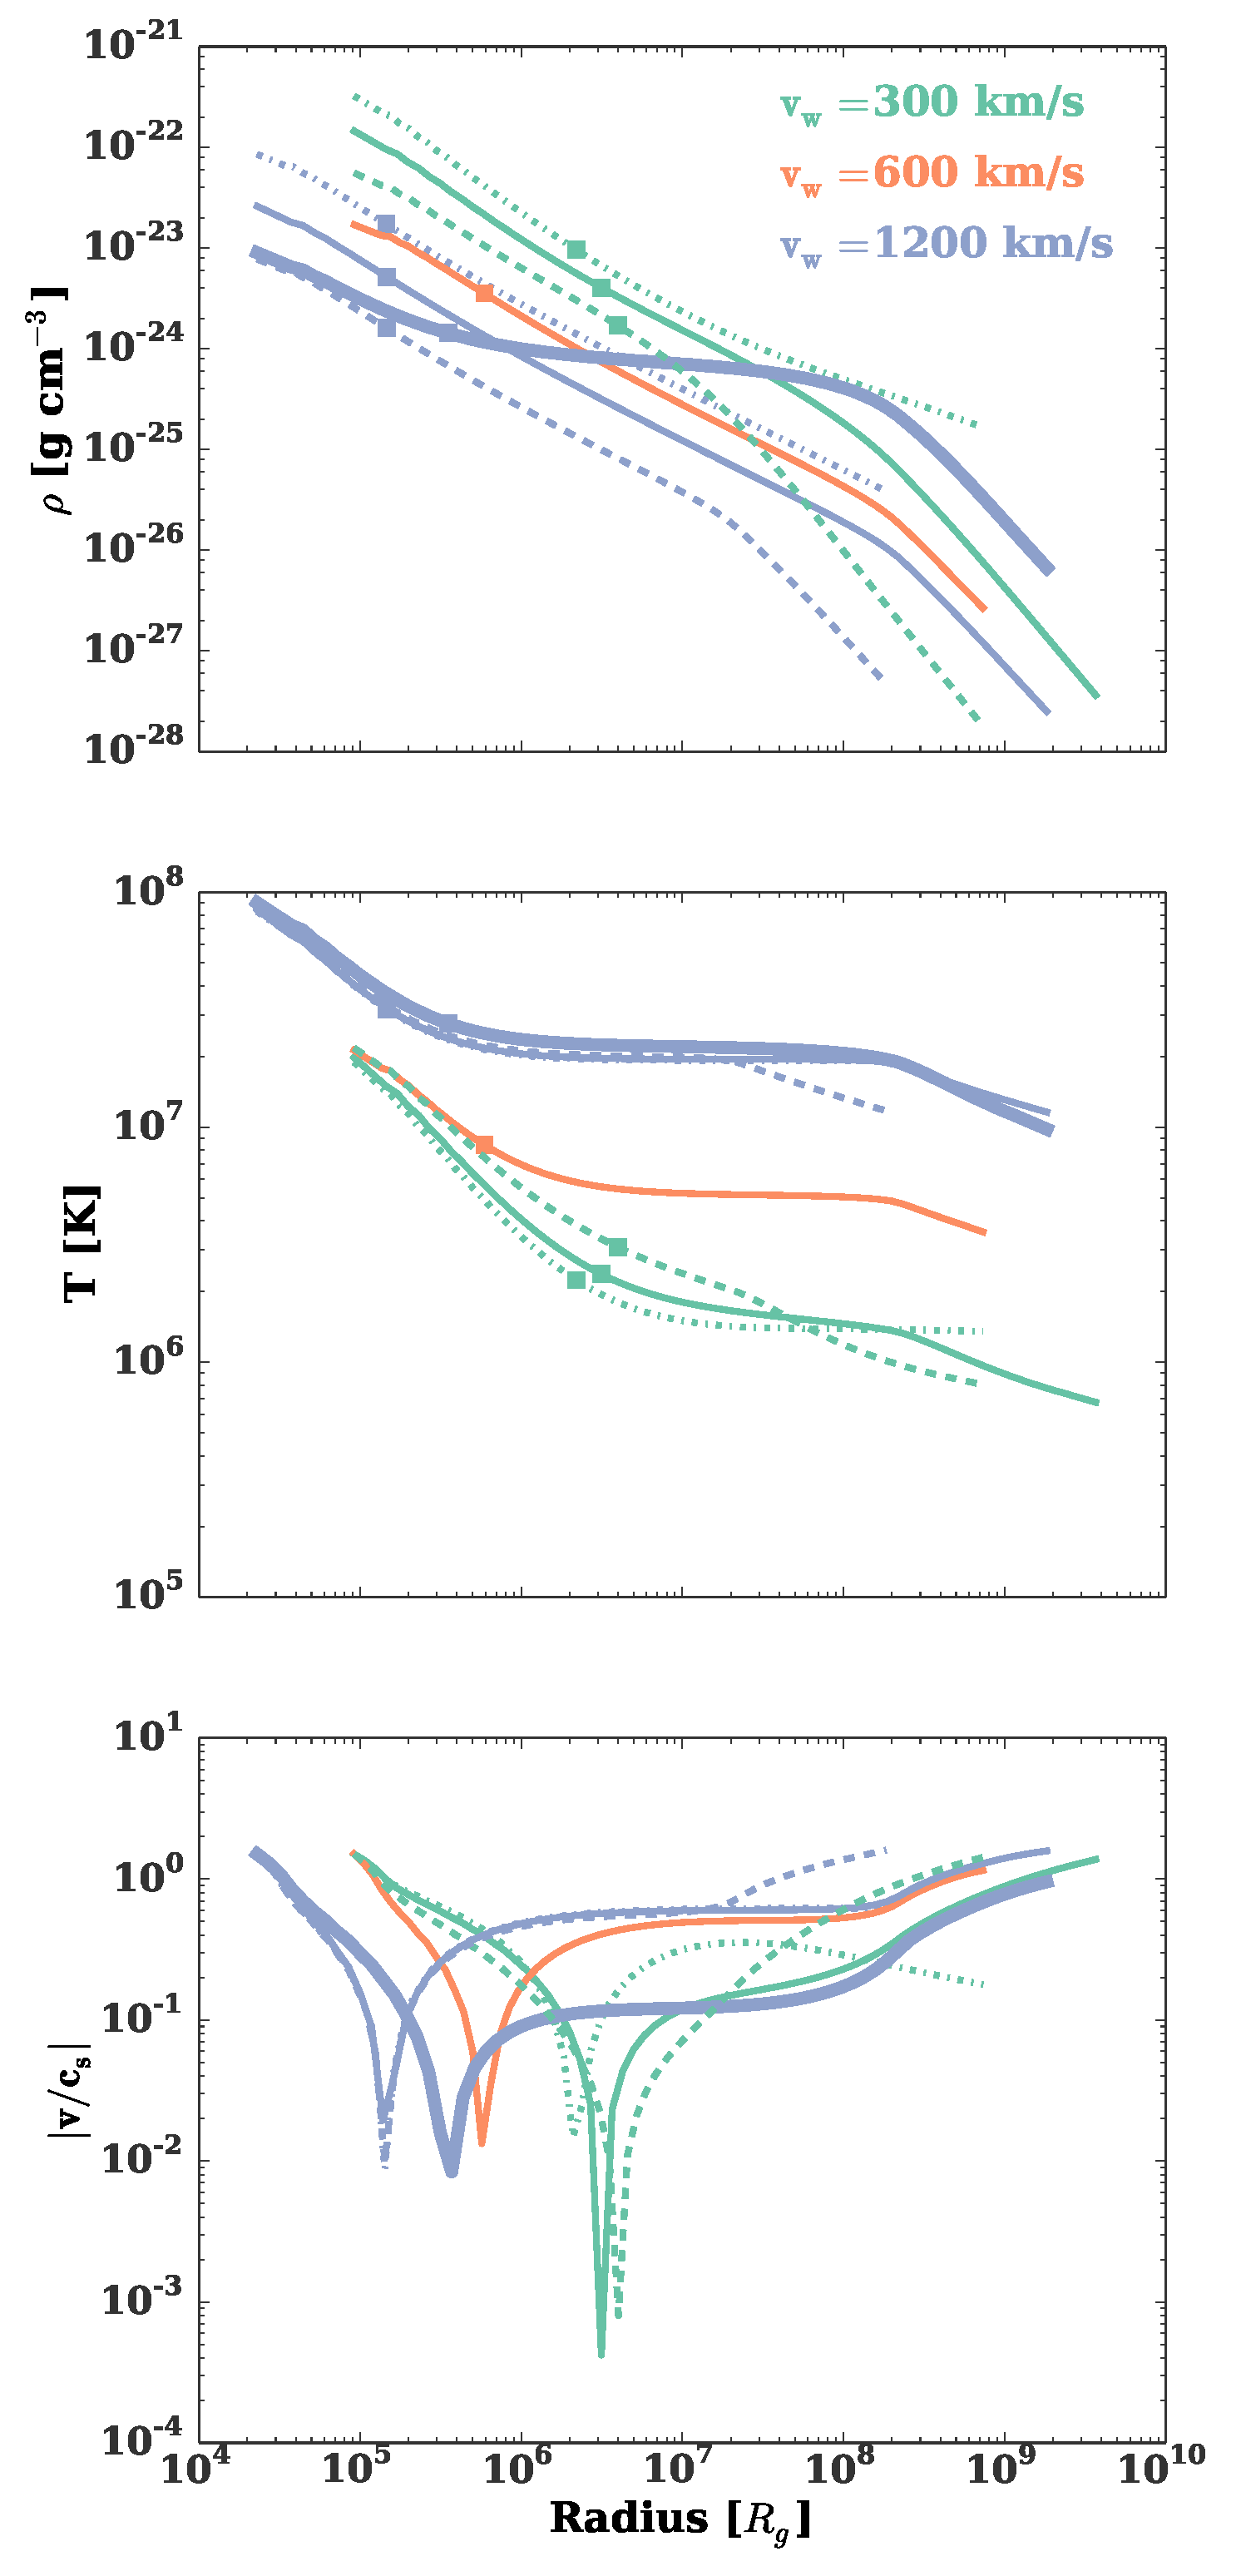
\includegraphics[width=\columnwidth]{profiles.eps}
  \caption{\label{fig:profiles}Radial profiles of the CNM density
    ({\it top}), temperature ({\it middle}), and velocity ({\it bottom}),
    calculated for a representative sample of galaxies.  Different colors
    denote different values of the effective wind heating rate,
    $\vwO=1200$ km s$^{-1}$ ({\it blue}), $\vwO$=600 km s$^{-1}$ ({\it
      orange}), and 300 km s$^{-1}$ ({\it green}).  Different
    linestyles correspond to different values of $\Mbh$, $\Mbh=10^6
    \Msun$ ({\it dot-dashed}), $\Mbh=10^7 \Msun$ ({\it solid}), and
    $\Mbh=10^8 \Msun$ ({\it dashed}). Thin lines correspond to cusp
    galaxies ($\Gamma$=0.8) and thick lines correspond to core
    galaxies ($\Gamma$=0.1). Squares mark the location of
    the stagnation radius for each solution {\bf BDM: added colored labels for the $v_w$ value, e.g. a blue 1200 km/s directly to the top figure.  what does v/cs look like?} .
 }
\end{figure}

  \subsection{Angular Momentum}
  \label{sec:ang}

Our spherically symmetric model neglects the effects of angular momentum on the gas evolution.  However, all galaxies possess some net rotation, resulting in centrifugal forces becoming important at some radius $r_{\rm circ} = l_{r_{s}}^{2}/(GM_{\bullet})$, where $l_{r_{s}} = r_{s}\langle V_{\phi}\rangle |_{r_s}$ is the specific angular momentum of stars near the stagnation radius, from which most of the accreted mass originates, and $\langle v_{\phi}\rangle$ is their average azimuthal velocity.    

Using two-dimensional kinematic data, \citet{EmsellemCappellari+:2007a} measure the ratio of ordered to random motion in a sample of early type galaxies, which they quantify at each galactic radius $R$ by the parameter
  \begin{align}
    \lambda_R=\frac{\langle R|V|\rangle}{\langle R\sqrt{V^2+\sigma^2}\rangle} \underset{R \ll r_{\rm soi}}\sim \frac{V_{\phi}}{\sigma},
  \end{align}
where $\sigma$ is the velocity dispersion and the brackets indicate a luminosity-weighted average.  The circularization radius of the accretion flow can be written in terms of $\lambda_R$ as
\be
\frac{r_{\rm circ}}{r_{s}} \approx \frac{r_{s}}{r_{\rm soi}}\lambda_{R}^{2} \lesssim \lambda_{R}^{2},
\label{eq:rcirc}
\ee
where we have used the definition $r_{\rm soi} \equiv GM_{\bullet}/\sigma^{2}$ and in the second inequality have assumed that $r_{\rm s} \lesssim r_{\rm soi}$ for the thermally-stable solutions of interest.

\citet{EmsellemCappellari+:2007a} (their Fig.~2) find that $\lambda_R < 0.1$ on scales less that 10 per cent of the galaxy radius, in which case equation (\ref{eq:rcirc}) shows that $r_{\rm circ} \lesssim 0.01r_{s}$.  Since this location lies well inside the inner sonic point of the flow, we conclude that angular momentum will only becomes important for thermally stable flows in a region that is causally disconnected from the rest of the flow, justifying its neglect in calculating quantities such as the mass accretion rate.


\section{Numerical Results}
\label{sec:numerical}

\begin{table*}
\begin{threeparttable}
%\centering
\begin{minipage}{18cm}
\caption{Summary of Numerical Solutions}
\begin{tabular}{lccccccccccccc}
\hline
{$M_{\bullet}$} & {$v_{w}$} & {$\Gamma^{(a)}$} & {$r_b^{(b)}$} &
{$\left(\frac{\dot{M}}{\dot{M}_{\rm edd}}\frac{0.04}{\eta}\right)_{r_{s}}^{(c)}$} & {$\left(\frac{t_{\rm cool}}{t_{\rm ff}}\frac{0.04}{\eta}\right)_{r_s}^{(d)}$} & TI?$^{(e)}$ \\
\hline
$(M_{\odot})$ & (km s$^{-1})$ & & (pc) & & &  & \\
\hline
$    10^{ 6 }$ & 300 & 0.8 & $>$ & $ 1.3 \times 10^{ -5 }$ & $ 1.2 \times 10^{ 2 }$ & No \\
$    10^{ 6 }$ & 600 & 0.8 & $>$ & $ 2.2 \times 10^{ -6 }$ & $ 8. 10^{ 3 }$ & No \\
$    10^{ 6 }$ & 1200 & 0.8 & $>$ & $ 3.8 \times 10^{ -7 }$ & $ 3.7 \times 10^{ 5 }$ & No \\
$    10^{ 7 }$ & 300 & 0.8 & 100 & $ 1.3 \times 10^{ -4 }$ & 6.5 & No \\
$    10^{ 7 }$ & 600 & 0.8 & 100 & $ 7.2 \times 10^{ -6 }$ & $ 2.4 \times 10^{ 3 }$ & No \\
$    10^{ 7 }$ & 1200 & 0.8 & $>$ & $ 1.3 \times 10^{ -6 }$ & $ 1.2 \times 10^{ 5 }$ & No \\
$    10^{ 8 }$ & 300 & 0.8 & 100 & $ 6.6 \times 10^{ -4 }$ & 1.4 & Yes \\
$    10^{ 8 }$ & 600 & 0.8 & 100 & $ 2.9 \times 10^{ -5 }$ & $ 5.3 \times 10^{ 2 }$ & No \\
$    10^{ 8 }$ & 1200 & 0.8 & 100 & $ 4.0 \times 10^{ -6 }$ & $ 3.8 \times 10^{ 4 }$ & No \\
$    10^{ 7 }$ & 300 & 0.8 & 50 & $ 7.9 \times 10^{ -5 }$ & 12 & No \\
$    10^{ 7 }$ & 300 & 0.8 & 200 & $ 1.2 \times 10^{ -4 }$ & 4.7 & Yes \\
$    10^{ 7 }$ & 300 & 0.8 & 400 & $ 3.6 \times 10^{ -4 }$ & 1.2 & Yes \\
$    10^{ 8 }$ & 300 & 0.8 & 50 & $ 3.3 \times 10^{ -4 }$ & 4.6 & Yes\\
$10^{8}\dagger$ & 300 & 0.8 & 50 & $ 9.1 \times 10^{ -4 }$ & 5.6 & Yes & \\
$    10^{ 8 }$ & 300 & 0.8 & 200 & $ 1.4 \times 10^{ -3 }$ & 0.43 & Yes \\
$    10^{ 6 }$ & 1200 & 0.1 & $>$ & $ 5.9 \times 10^{ -8 }$ & $ 1.0 \times 10^{ 6 }$ & No \\
$    10^{ 7 }$ & 1200 & 0.1 & $>$ & $ 3.8 \times 10^{ -7 }$ & $ 1.4 \times 10^{ 5 }$ & No \\
$    10^{ 8 }$ & 1200 & 0.1 & 100 & $ 2.4 \times 10^{ -6 }$ & $ 2. 10^{ 4 }$ & No \\
$    10^{ 8 }$ & 1200 & 0.1 & 50 & $ 2.0 \times 10^{ -6 }$ & $ 3. 10^{ 4 }$ & No \\
$    10^{ 8 }$ & 1200 & 0.1 & 200 & $ 4.2 \times 10^{ -6 }$ & $ 8.4 \times 10^{ 3 }$ & No \\
$    10^{ 8 }$ & 1200 & 0.1 & 400 & $ 1.2 \times 10^{ -3 }$ & 4.6 & Yes \\
\hline
\label{table:models}  
\end{tabular}
\begin{tablenotes}
\item $^{(a)}$ Inner power-law index of stellar Nuker profile.  $^{(b)}$
Break radius of stellar Nuker profile.  $^{(c)}$Accretion rate in
Eddington units, normalized to a stellar mass input parameter $\eta =
0.04$.  $^{(d)}$Ratio of cooling timescale to free-fall timescale at
stagnation radius.  Thermally unstable solutions are shown in bold text.  $^{(e)}$ Is solution thermally unstable?
$\dagger$Calculated including radiative cooling, assuming $\eta =
0.04$.  {\bf  BDM: (3) make sure all combinations of vw and mbh
  are included. AG: Realized that the solution I ran earlier, with
  cooling was actually a solution that would be thermally unstable
  according to our thermal instability. I am worried that this
  solution may not be representative due to the small break radius. BDM: change TI column to simply bolding tcool ratio in those cases which are thermally unstable.}
\end{tablenotes}
\end{minipage}
\end{threeparttable}

\end{table*}




%\begin{table*}
%\centering
%\begin{minipage}{18cm}
%\caption{Comparison of numerical solutions with and without
 % cooling. We have chosen $\eta=0.04$, which one would expect for 
  %the average star formation history for $\Mbh=10^8\Msun$ 
 % (see Figures~\ref{fig:eta} {\bf AG-cite star formation history
  %  figure once it is made.}). Note that we have deliberately chosen a solution
  %near our thermal stability threshold where cooling is beginning
  %to become important.
%}
%\begin{tabular}{lccccccccccccc}
%\hline
%{$M_{\bullet,8}$} & {$v_{w}$} & {$\Gamma$} & {$r_b$} & {$\eta$} &
%{$\dot{M}/\dot{M}_{\rm edd}$} & {$(t_{\rm cool}/t_{\rm ff})_{r_s}$} & {comments}\\
%\hline
%1 & 300 & 0.8 & 50.0 & 0.04 & $ 3.3 \times 10^{ -4 }$ & 4.6 &  \\
%1 & 300 & 0.8 & 50.0 & 0.04 & $ 9.1 \times 10^{ -4 }$ & 5.6 & \\
%\hline
%\label{table:models}  
%\end{tabular}
%\end{minipage}
%\end{table*}

Our numerical results, summarized in Table \ref{table:models} and Figure XXX, allow us to study a range of CNM properties and to assess the validity of the analytic estimates from the previous section.  Cases for which $(\dot{q}_{\rm heat}/|\dot{q}_{\rm rad}|)< 1$ at the stagnation radius are marked as `thermally unstable', as are cases for which the stagnation radius diverges and hence could not be resolved, resulting in their calculations being terminated.  

Figure~\ref{fig:profiles} shows profiles of the density $\rho(r)$,
temperature $T(r)$, and radial velocity $|v(r)|$, for the cusp
($\Gamma=0.8$) solutions within our grid.  As expected, the gas
density increases towards the SMBH $\rho\propto r^{-n}$ with
$n\simeq1$, i.e. shallower than the $-3/2$ power law for
Bondi accretion. This power law behavior does not extend
through all radii, however, as the gas density profile has a break coincident
with the location of the break in the stellar light profile ($\rb=100$
pc). The temperature profile is relatively flat at large radii, but
increases as $\propto 1/r^{k}$ interior to the sphere of influence,
where $k\lesssim 1$, somewhat shallower than expected for virialized gas within the black hole sphere of influence.
The inwardly directed velocity increases towards the hole with a profile that is somewhat steeper than the local free-fall velocity $v \propto v_{\rm ff}\propto r^{-1/2}$.
% {\bf BDM: I made this up - in general we need
%   more explanation of what the plots are actually showing, with some
%   physical explanation.}
% AG -- things are not quite approaching Bondi on the inner grid. I
% don't have a good physical explanation yet...

Figure~\ref{fig:stag} shows our results for the stagnation radius $r_{\rm s}$, expressed in ratio to sphere of influence radius $r_{\rm soi}$, with different colors showing different values of $v_{w}$.  Cusp and core galaxies are marked with square and triangles, respectively.  Shown for comparison are our analytic results (eq.~[\ref{eq:rs2main}]) with solid and dashed lines for cusp and core galaxies, respectively, calculated assuming $n = 1$ and $n= 0.5$, respectively.  Our analytic estimates are found to provide accurate fits to the numerical results for $v_{\rm w} \gtrsim \sigma$, but the assumptions leading to these estimates become invalid for low $v_{\rm w}$ as the stagnation radius diverges to large radii.  For $v_{w} \gg \sigma$ the ratio $\rs/\rsoi$ does not depend sensitively on break radius $r_{b}$, but the latter has a greater influence when $v_{w} \lesssim \sigma$.  The three green squares which are vertically aligned at the same value of $v_{w}/\sigma$ (close to where the analytic estimate diverges) correspond to models with the same black hole mass ($\Mbh = 10^7 \Msun$) and heating rate ($v_w = 300$ km s$^{-1}$) but different values of the break radius: $r_{b} = $ 50, 100, and 400 pc (from top to bottom).  As $r_{\rm b} \rightarrow r_{s}$, the effects of the break radius is to the push the stagnation radius inwards, decreasing the SMBH accretion rate.    
%% AG: Describe conservation checks to additionally validate the results.

\begin{figure}
  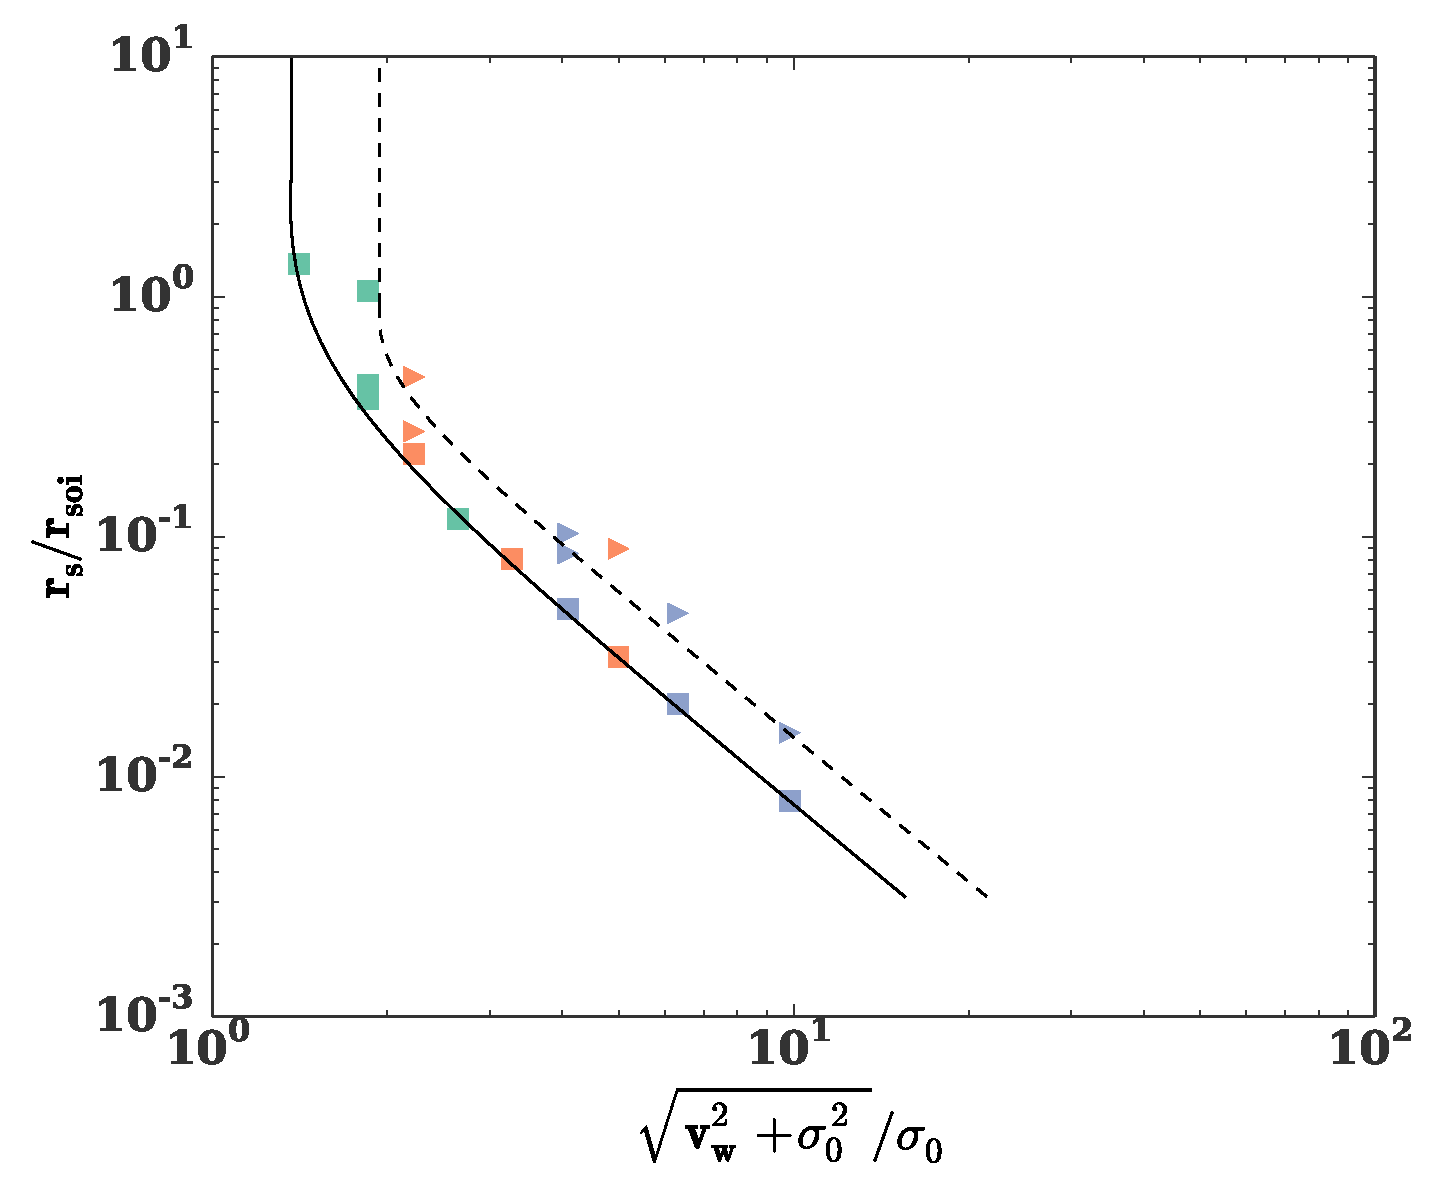
\includegraphics[width=\columnwidth]{rs.eps}
  \caption{\label{fig:stag} \emph{Top panel:} Stagnation radius
    $r_{s}$ in units of the sphere of influence radius $r_{\rm
      soi}$ (eq.~[\ref{eq:rsoi}]) for galaxies in our sample as a
    function of the ratio of the effective wind heating rate $v_{w}$
    to the stellar velocity dispersion $\sigma$.  Green, orange, and
    blue symbols correspond to different values of $v_{w} =$ 300, 600, and 1200 km s$^{-1}$,
    respectively.  Squares correspond to cusp galaxies ($\Gamma = 0.8$), while
    triangles correspond to cores ($\Gamma = 0.1$). The black curves correspond to the
    analytic prediction from equation (\ref{eq:rs2main}), with solid and dashed curves calculated for parameters $\{\Gamma=0.8, n=1\}$ and $\{\Gamma=0.1,n=0.5\}$, respectively. }
\end{figure}


\begin{figure}
  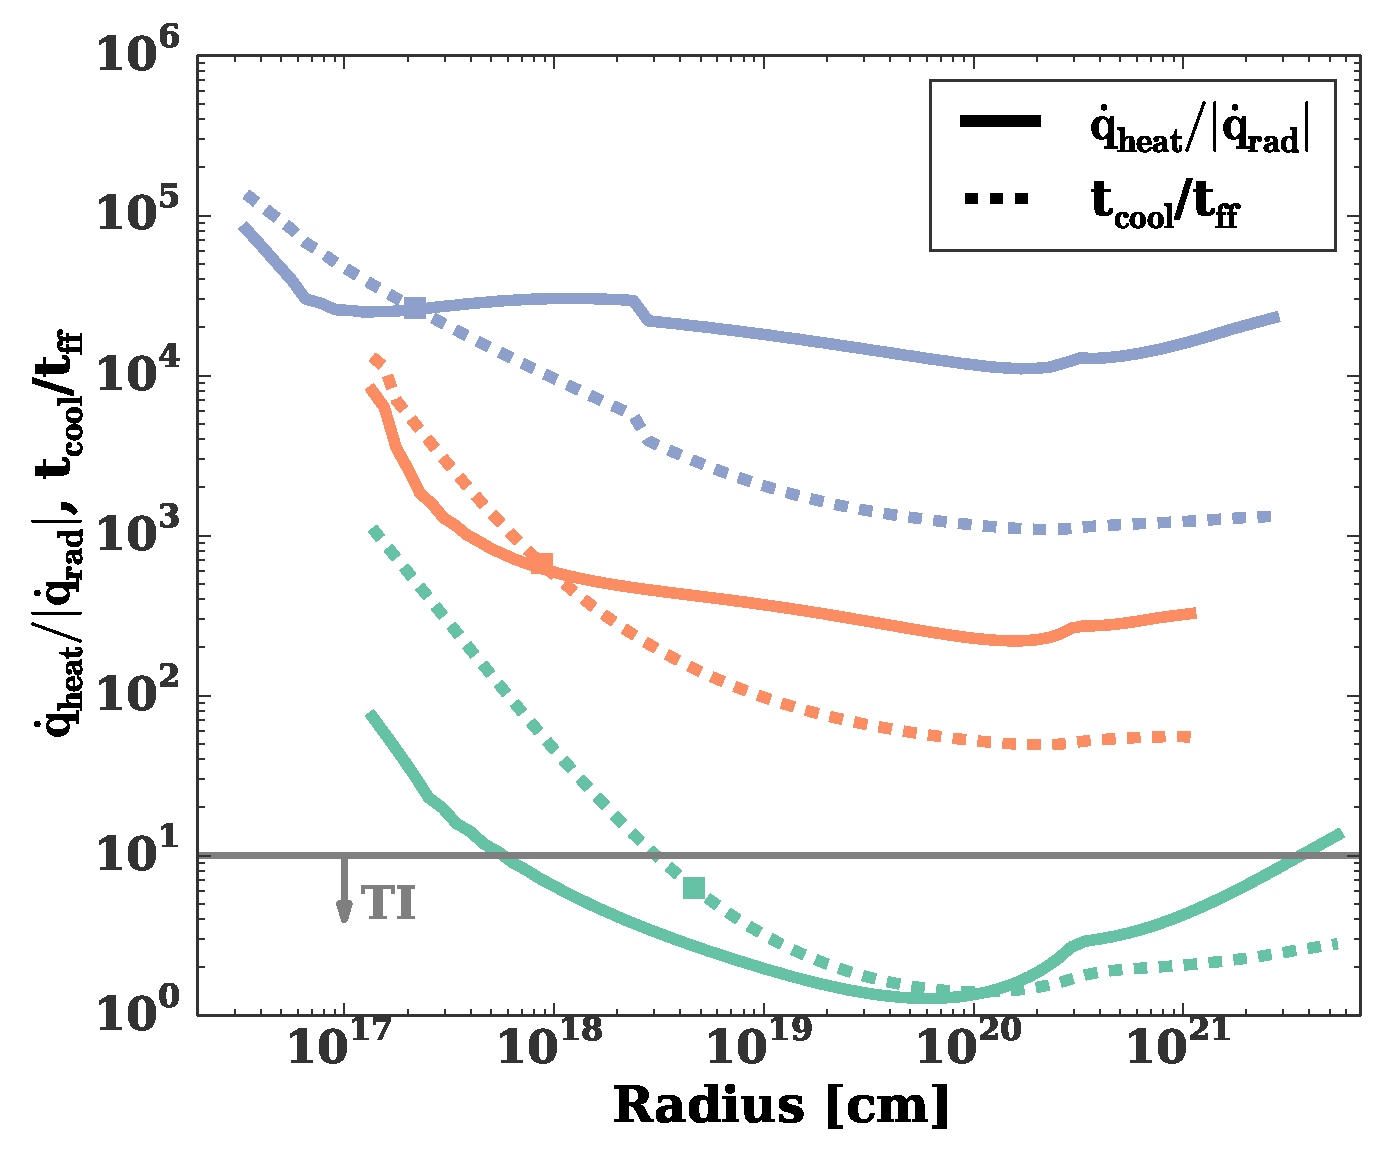
\includegraphics[width=\columnwidth]{cooling.eps}
  \caption{\label{fig:cooling} Ratio of the rate of heating to
radiative cooling, $\dot{q}_{\rm heat}/|\dot{q}_{\rm rad}|$, as a
function of radius (solid lines) for each of our solutions shown in
Figure \ref{fig:profiles}.  Dashed lines show for comparison the ratio
of the cooling to the free-fall timescale $t_{\rm cool}/t_{\rm ff}$.
For high heating rates both ratios are approximately equal at the
stagnation radius (marked as squares).  When $\dot{q}_{\rm
heat}/\dot{q}_{\rm cool} \lesssim 1$ and/or $t_{\rm cool}/t_{\rm ff}
\lesssim 10$, the flow is susceptible thermal instabilities.  {\bf
BDM: change y axis labels to qdotheat/qdotrad, tcool/tff}.}
\end{figure}


Fig.~\ref{fig:cooling} shows the ratio of wind heating to radiative cooling, $\dot{q}_{\rm heat}/|\dot{q}_{\rm rad}|$ (eq.~[\ref{eq:cooling2}] and surrounding discussion) as a function of radius for our fiducial solutions shown in Figure \ref{fig:profiles}.  For high heating rates of $v_{w} = 600$ and $1200$ km s$^{-1}$ cooling is unimportant across all radii, while for $v_{w} = 300$ km s$^{-1}$ we see that $\dot{q}_{\rm heat}/|\dot{q}_{\rm rad}|$ and $\tcool/\tff$ can be less than unity, depending on the wind mass loss parameter $\eta$.  At the stagnation radius, the ratio $\dot{q}_{\rm heat}/|\dot{q}_{\rm rad}|$ reaches a value that lies within a factor of two of its minimum across the entire grid;  thus, the value of $(\dot{q}_{\rm heat}/|\dot{q}_{\rm rad}|)_{r_{s}}$ provides a diagnostic of thermal instabilty for the entire solution.  

Also note that for $v_{w}=600$ and $1200$ km s$^{-1}$ we have that $\dot{q}_{\rm heat}/|\dot{q}_{\rm rad}| \sim t_{\rm cool}/t_{\rm ff}$ near the stagnation radius.  However, the two ratios diverge from each other at low heating ($v_{w} \lesssim 300$ km s$^{-1}$) because equations (\ref{eq:mdot_gas}), (\ref{eq:rhors}) underestimate the true gas density, which is greater in a subsonic inflow (weak heating) than in a supersonic outflow (strong heating).  

\section{Sources of Heating}
\label{sec:heating}

Key properties of the flow, such as the SMBH accretion rate and the likelihood of thermal instability depend sensitively on the assumed heating rate $\propto qv_{w}^{2}$.  This section summarizes individual heating sources, providing estimates of the value of
\begin{align}
  v_{w} = \sqrt{\frac{2 t_h \dot{e}}{\eta \rhostar}}
  \label{eq:vw_eff}
\end{align}
for each, where $\dot{e}$ is volumetric heating rate.  

\subsection{Stellar winds} 

Energy and mass input to the CNM by stellar winds is the sum of contributions from main sequence and post-main sequence populations.  At early times following star formation, energy input is dominated by core collapse supernovae and by the fast outflows of Wolf-Rayet stars (e.g., \citealt{VossDiehl+:2009a}).  At later times energy input is dominated by main sequence winds (e.g., \citealt{NaimanSoares-Furtado+:2013a}).  Mass input is also dominated by massive stars for very young stellar populations, but for most stellar ages the slow AGB winds of evolved low-mass stars dominate the mass budget.  

In Appendix \ref{app:windheat} we calculate the wind heating rate from
stellar winds, $v_{\rm w}^{\star}$, and the mass loss parameter,
$\eta$ (eq.~[\ref{eq:q}]), as a function of age, $\tau_{\star}$, of a
stellar population which is formed impulsively (Fig.~\ref{fig:vwimp}).
At the earliest times ($\tau_{\star} \lesssim 10^{7}$ yr), the wind
heating rate exceeds 1000 km s$^{-1}$, while much later ($\tau_{\star}
\sim t_{\rm h}$) stellar wind heating dominated by main sequence winds
is much lower, $v^{\star}_{\rm w} \sim 50-100 $ km s$^{-1}$.  We show
in $\S\ref{sec:combined}$ that for the case of quasi-continueous star
formation representative of the average star formation history of loss
mass galaxies, the stellar wind heating rate produced by stellar winds
can also be significant, $v_{\rm w}^{\star} \gtrsim 1000$ km s$^{-1}$.
Stellar winds thus contribute a potentially important source of both
energy and mass for the CNM.

\subsection{Type Ia Supernovae} 

Type Ia supernovae (SNe Ia) represent a potentially important source of heating, which unlike core collapse SNe is present even in an evolved stellar population.  If each Ia supernova injects thermal energy $E_{\rm Ia}$ into the interstellar medium, and the SNe rate (per stellar mass) is given by $R_{\rm   Ia}$, then the resulting volumetric heating rate of $E_{\rm Ia}R_{\rm  Ia}$ produces an effective wind heating parameter (eq.~[\ref{eq:vw_eff}]) of \begin{align} v_{w}^{\rm Ia} =\sqrt{\frac{2 t_h R_{\rm Ia}
E_{\rm Ia}}{\eta}} \label{eq:vw_sne}.
\end{align} The thermal energy injected by each SN Ia, $E_{\rm Ia} \simeq
\epsilon_{\rm Ia} 10^{51}$ erg, depends on the efficiency $\epsilon_{\rm Ia}$
with which the initial blast wave energy is converted into bulk or turbulent
motion instead of being lost to radiation.  \cite{Thornton+98}
estimate a radiative efficiency $\epsilon_{\rm Ia} \sim 0.1$,
depending weakly on surrounding density, but \citet{Sharma+14} argues
that $\epsilon_{\rm Ia}$ can be considerably higher, $\sim 0.4$, if
the SNe occur in a hot dilute medium, as may characterize the circumnuclear medium.  Hereafter we adopt $\epsilon_{\rm Ia} = 0.4$ as fiducial.

The SN Ia rate, $\RateIa$, depends on the age of the stellar population, as it represent the convolution of the star formation rate and the Ia delay time distribution (DTD) divided by the present stellar mass.  In
the limit of impulsive star formation, $\RateIa$ is the DTD evaluated at the time since the star formation episode.  The observationally-inferred DTD (Fig. 1 of \citealt{MaozMannucci+:2012a}) has the
approximate functional form \begin{align}
  R_{\rm Ia} =1.7\times 10^{-14}\left(\tau_{\star}/t_{\rm
      h}\right)^{-1.12} M_{\odot}^{-1}\,{\rm yr^{-1}}
\label{eq:DTD}
  \end{align}
  where $\tau_{\star}$ is the time since star formation
  (c.f.~\citealt{Scannapieco&Bildsten05}). 

From equations (\ref{eq:vw_sne}), (\ref{eq:DTD}) we thus estimate that 
  \begin{eqnarray} 
    v_{w}^{\rm Ia} &\approx& 700(\epsilon_{\rm
      Ia}/0.4)^{0.5}(\tau_{\star}/t_{\rm h})^{-0.56}\eta_{0.02}^{-1/2}\,{\rm km
      \,s^{-1}} \nonumber \\
&\approx& 700(\epsilon_{\rm
      Ia}/0.4)^{0.5}(\tau_{\star}/t_{\rm h})^{0.09}\,{\rm km
      \,s^{-1}},
\label{eq:vIa}
  \end{eqnarray}
where the second line assumes $\eta\simeq 0.02 (\tau_{\star}/t_h)^{-1.3}$ for a single burst of star formation (e.g. , \citealt{Ciotti+91}).

The high value of $v_{w}^{\rm Ia}$ implies that Ia SNe represent an
important source of CNM heating.  However, SNe can only be
approximated as supplying heating which is spatially and temporally
homogeneous if the rate of SNe is rapid compared to the characteristic
evolution time of the flow at the radius of interest
(\citealt{ShcherbakovWong+:2014a}).  We define the ``Ia radius"
  \begin{align}
    r_{\rm Ia} \sim \left(\frac{G}{R_{\rm Ia}\sigma}\right)^{1/2} \sim
    38 M_{\bullet,8}^{-0.1}(\tau_{\star}/t_{\rm h})^{0.56}\,{\rm pc}
    \label{eq:rIa}
  \end{align}
  as the location exterior of which the time interval between
  subsequent supernovae $\tau_{\rm Ia} \sim (M_{\rm enc}R_{\rm
    Ia})^{-1} \sim G/(r\sigma^{2}R_{\rm Ia})$ exceeds the local
  dynamical timescale $t_{\rm dyn} \sim r/\sigma$, where we again
  adopt the Ia rate for an old stellar population and in the final
  equality we estimate the velocity dispersion using the
  $M_{\bullet}-\sigma$ relationship (eq.~[\ref{eq:Msigma}]).

Assuming that $v_{w}^{\rm Ia} \gg \sigma$ then by substituting
$v_{w}^{\rm Ia}$ (eq.~\ref{eq:vIa}) into equation (\ref{eq:rs_simple})
for the stagnation radius, we find that

\begin{eqnarray}
  \left.\frac{r_{\rm Ia}}{r_{\rm s}}\right|_{\rm v_{w}^{\rm Ia}}
  &\approx& 12\eta_{0.02}^{-1} M_{\bullet,8}^{-1.1}(\epsilon_{\rm
    Ia}/0.4) (\tau_{\star}/t_{\rm h})^{-0.56} \nonumber \\
  &\approx& 12 M_{\bullet,8}^{-1.1}(\epsilon_{\rm Ia}/0.4) (\tau_{\star}/t_{\rm h})^{0.74}
\label{eq:rIars}
\end{eqnarray}
{\bf AG-Note the different scaling relations here.}
If $r_{\rm Ia} \gg r_{\rm s}$, then Ia heating can only be
approximated as a steady heating source near the stagnation radius for
extremely massive SMBHs with $M_{\bullet} \gtrsim 10^9 \Msun$ or in
the case of a very young stellar population ($\tau_{\star} \ll t_{\rm
h}$).  On the other hand, equation (\ref{eq:rIars}) may underestimate
the importance of Ia heating because $r_{\rm Ia}/r_{\rm s}$ will be
substantially smaller than its value estimated using $v_{w}^{\rm Ia}$
if the heating rate excluding SN Ia is less than this.

Even if SN Ia are rare near the stagnation radius, they may cap the
SMBH accretion rate by periodically blowing gas out of the nucleus of
low mass galaxies.  Between subsequent supernovae, stars release a
gaseous mass $M_{\rm g} \approx \eta M_{\star}\tau_{\rm Ia}/t_{\rm h}$
interior to the Ia radius, which is gravitationally bound to the SMBH
by an energy $E_{\rm bind} \sim M_{\rm g}\sigma^{2}$.  Thus, according
to the above definitions, $E_{\rm Ia}/E_{\rm bind} \sim (v_{w}^{\rm
  Ia})^{2}/2\sigma^{2} \gtrsim 1$.  Hence, SN Ia are in principle
capable of dynamically clearing out gas from radii $\sim r_{\rm Ia}
\gtrsim r_{\rm s}$, at least for low mass BHs with $\sigma \ll v^{\rm
  Ia}_{w}$.  Thus, even in cases when heating is sufficiently weak
that the stagnation radius formally exceeds $r_{\rm Ia}$, the
accretion rate is limited to a maximum value,
\begin{eqnarray}
\frac{\dot{M}_{\rm Ia}}{\dot{M}_{\rm edd}} &\approx& \frac{\eta M_{\bullet}}{\dot{M}_{\rm edd} t_{\rm h}}\left(\frac{R_{\rm Ia}}{R_{\rm soi}}\right)^{2-\Gamma} \approx \nonumber \\
 && \begin{cases}
    4.5 \times 10^{-4} M_{\bullet,8}^{-1.33}(\tau_{\star}/t_{\rm h})^{-0.2}
   & \text{core} \\
    2.2 \times 10^{-4} \Mbheight^{-0.84}(\tau_{\star}/t_{\rm h})^{-0.6}   & \text{cusp},
  \end{cases}
  \label{eq:eddr_Ia}
\end{eqnarray}
obtained substituting the Ia radius $r_{\rm Ia}$ (eq.~[\ref{eq:rIa}]) for $r_{\rm s}$ in the derivation leading to our estimate of $\dot{M}$ (eq.~[$\ref{eq:eddr_analytic}$]).  Note that $\dot{M}_{\rm Ia}$ usually exceeds the maximum accretion rate for a thermally stable flow $\dot{M}_{\rm TI}$ (eq.~[\ref{eq:Mdotmax}]), implying that dynamical `blow-out' from SNe Ia cannot alone prevent cooling instabilities in the nuclei of low mass galaxies.  Also note that Ia supernovae only cap the accretion rate to this maximum value if the gas feeding the black hole is supplied by local stellar mass loss: the gaseous mass can become much greater if the nucleus is fed externally, e.g. due to a galaxy merger or to cooling flows developing within the galaxy over much longer timescales (e.g.~\citealt{Ciotti&Ostriker07}). 



\subsection{Millisecond Pulsars}
 Energy injection from the spin-down of millisecond pulsars (MSPs) is a potentially
important heating source.  If the number of MSPs per unit stellar mass
is $n_{\rm msp}$ and each contributes on average a spin-down
luminosity $\bar{L}_{\rm sd}$, then the resulting heating per unit
volume $\dot{e} \approx \bar{L}_{\rm sd}n_{\rm msp}\epsilon_{\rm msp}$ results in an
effective heating rate (eq.~ [\ref{eq:vw_eff}]) of 
\begin{eqnarray} v_{w}^{\rm MSP} \sim
30\left(\frac{\epsilon_{\rm msp}}{0.1}\right)^{1/2}\left(\frac{\bar{L}_{\rm
sd}}{10^{34}\,{\rm erg\,s^{-1}}}\right)^{1/2} \eta_{0.02}^{-1/2}\,{\rm
km\,s^{-1}},
 \label{eq:vmsp}
  \end{eqnarray} 
where $\epsilon_{\rm msp}$ is the thermalization efficiency of
the wind, normalized to a value $\lesssim 0.1$ based on that inferred by modeling the interstellar media of globular clusters
\citep{NaimanSoares-Furtado+:2013a}.  Our numerical estimate assumes a
pulsar density $n_{\rm msp} \sim 3 \times 10^{-40} $ MSPs g$^{-1}$, calculated from the estimated $\sim 30,000$ MSPs in the Milky Way (\citealt{Lorimer13}) of stellar mass $\approx 6\times 10^{10}M_{\odot}$.

Based on the ATNF radio pulsar catalog (\citealt{Manchester+05}), we estimate the average spin-down luminosity of millisecond pulsars in the field to be $\bar{L}_{\rm sd} \sim 10^{34}$ erg s$^{-1}$, resulting in $v_{w}^{\rm MSP} \lesssim 30$ km s$^{-1}$ for $\eta \gtrsim 0.02$.  For higher spin-down
luminosities, $L_{\rm sd}\simeq 10^{35}$ ergs s$^{-1}$ characteristic
of some Fermi-detected pulsars, then the higher value of $v_{w}^{\rm MSP}
\lesssim 300$ km s$^{-1}$ makes MSP heating in principle important
under the most optimistc assumptions $\epsilon_{\rm msp} = 1$ and $\eta = 0.02$.  On the other hand, it seems likely that the stellar binaries giving rise to MSPs could be disassociated by stellar interactions in the dense nuclear cluster, reducing the numbers of MSPs as compared to the field population estimate above.  


\subsection{SMBH Feedback}

Feedback from accretion onto the SMBH represents an important source of heating which, however, is also the most difficult to quantify (e.g., \citealt{Brighenti&Mathews03}, \citealt{DiMatteo+05}; \citealt{Kurosawa&Proga09}; \citealt{Fabian12} for a recent review).  A key difference between AGN heating and the other sources discussed thus far is its dependence on the SMBH accretion rate $\dot{M}$, which is itself a function of the heating rate (eq.~[\ref{eq:mdot_analytic}]).  

\subsubsection{Compton Heating}

There are two types of SMBH feedback: kinetic and radiative.  Radiative feedback is potentially effective even in low luminosity AGN via Compton heating (e.g., \citealt{Sazonov+04}, \citealt{Ciotti+10}), which provides a volumetric heating rate (\citealt{Gan+14})
\be
\dot{e} = 4.1\times 10^{-35}n^{2}\xi T_{\rm C}\,{\rm erg\,cm^{-3}\,s^{-1}},
\ee
where $\xi = L/n r^{2}$ is the ionization parameter and $L$ is the SMBH luminosity with Compton temperature $T_{\rm C} \sim 10^{9}$ K $\gg T$ (e.g., \citealt{Ho99}, \citealt{Eracleous+10}).  

The importance of Compton heating can be estimated by assuming the SMBH
radiates with a luminosity $L = \epsilon_{\rm rad} \dot{M}c^{2}$, where
$\epsilon_{\rm rad}$ is the radiative efficiency and where $\dot{M}$ is
estimated from equation (\ref{eq:mdot_analytic}).  Then using
equations (\ref{eq:rs_simple}), (\ref{eq:mdot_analytic}),
(\ref{eq:rhors}), (\ref{eq:rhostarrs}) we calculate that from equation
(\ref{eq:vw_eff}) that the effective heating rate at the stagnation radius is given by
\begin{align} v_{w}^{\rm C} \simeq
  \begin{cases} 29 \eta_{0.02}^{0.5}T_{\rm
C,9}^{0.5}\epsilon_{-2}^{0.5} M_{\bullet,8}^{0.38}v_{500}^{-1.4}\,{\rm
km\,s^{-1}} &, \text{core}\\ 50 \eta_{0.02}^{0.5}T_{\rm
C,9}^{0.5}\epsilon_{-2}^{0.5} M_{\bullet,8}^{0.24}v_{500}^{-0.7}\,{\rm
km\,s^{-1}} &, \text{cusp},
  \end{cases}
  \label{eq:vC}
\end{align} where $T_{C,9} = T_{C}/10^{9}$ K and $\epsilon_{-2} =
\epsilon_{\rm rad}/0.01 \sim 1$ is the maximum radiative efficiency
for an advective accretion flow expected to produce high $T_{\rm C}$
emission (e.g.~\citealt{Narayan&Yi95}).  We caveat that, unlike stellar wind heating, Compton heating depends on radius, scaling as $v_{w}^{\rm C}(r) \propto (n^{2}\xi/\rho_{\star})^{1/2} \propto r^{(\Gamma-n-1)/2}$, i.e. $\propto r^{-0.6}$ and $\propto r^{-0.7}$ for core ($\Gamma = 0.8$; n = 1) and cusp ($\Gamma = 0.1$; n = 0.5) galaxies, respectively.  The assumption of our model that the heating parameter be constant with radius is not satisfied, but this radial variation is sufficiently weak that it should not significantly alter our conclusions.  

If Compton heating acts alone, i.e. $\tilde{v}_{w} = v_{w}^{C}$, then solving equation
(\ref{eq:vC}) for $\tilde{v}_{\rm w}$ yields
\begin{align} v_{w}^{\rm C} \simeq
  \begin{cases} 150 \eta_{0.02}^{0.21}T_{\rm
C,9}^{0.21}\epsilon_{-2}^{0.21} M_{\bullet,8}^{0.16}\,{\rm km\,s^{-1}}
&, \text{core}\\ 130 \eta_{0.02}^{0.29}T_{\rm
C,9}^{0.29}\epsilon_{-2}^{0.29} M_{\bullet,8}^{0.14}\,{\rm km\,s^{-1}}
&, \text{cusp},
  \end{cases}
  \label{eq:vC2}
\end{align} 
Compton heating can thus be significant in young stellar populations with relatively high mass loss rates, e.g. $v_{w}^{\rm C} \gtrsim 300$ km s$^{-1}$ for $\eta \gtrsim 1$.  


\subsubsection{Kinetic Feedback}

Kinetic feedback results from outflows of energy or momentum from close to the black hole in the form of a disk wind or jet, which deposits its energy as heat, e.g. via shocks or wave dissipation, over much larger radial scales (e.g.~\citealt{McNamara&Nulsen07}; \citealt{Novak+11}; \citealt{Gaspari+12}).  

Assume that the outflow power is proportional to the SMBH accretion rate, $L_{\rm j} =
\epsilon_{\rm j} \dot{M}c^{2}$, where $\epsilon_{\rm j} < 1$ is a jet efficiency factor.  Further assume that this energy is deposited as heat uniformly interior to a radius $r_{\rm heat}$ and volume $V_{\rm heat} \propto r_{\rm
heat}^{3}$.  The resulting volumetric heating rate $\dot{e} = \epsilon_{\rm
j}\dot{M}c^{2}/V_{\rm heat}$ near the stagnation radius results in a heating parameter given by
\begin{eqnarray} v_{w}^{\bullet} &\approx& \left(\frac{2t_{\rm
h}\epsilon_{\rm j}\dot{M}c^{2}}{V_{\rm heat}\eta
\rho_{\star}}\right)^{1/2} \sim \left(\frac{\epsilon_{\rm
j}\dot{M}c^{2}t_{\rm h}}{\eta M_{\rm enc}}\right)^{1/2} \nonumber \\
&\approx& 300\,{\rm km\,s^{-1}}\,\left(\frac{\epsilon_{\rm j}}{10^{-6}}\right)^{1/2}\left(\frac{r_{\rm s}}{r_{\rm
heat}}\right)^{1-\Gamma/2},
\label{eq:vjet}
\end{eqnarray} 
where we have used the facts that $\dot{M} = \eta M_{\star}|_{r_{\rm s}}/t_{\rm h}$ and, for radii inside the Nuker break radius, $M_{\star}(r) \propto
M_{\bullet}(r/r_{\rm soi})^{2-\Gamma}$ (eq.~[\ref{eq:rhostar}]).  If the bulk of the outflow energy is released near the stagnation radius, then even a small heating efficiency $\epsilon_{\rm j} \gtrsim
10^{-5}$ is sufficient for $v_{w}^{\bullet}$ to exceed other sources of non-accretion powered heating.  However, if this energy is deposited over much larger physical scales comparable to the size of the galaxy, i.e. $r_{\rm heat} \gtrsim $ 10 kpc $\sim 10^{4}r_{\rm s}$, then kinetic feedback is unimportant, even for a powerful jet with $\epsilon_{\rm j} \sim 1$.  

Using the results of \citet{Bromberg+11}, the time required for a jet of luminosity $L_{\rm
  j}$ and half opening angle $\theta_{\rm j} = 0.1$ (characteristic of
AGN jets) to propagate through a gaseous mass $M_{\rm g}$ of radius $r$ is estimated to be
\begin{eqnarray}
t_{\rm jet} &\sim& 4000\,{\rm yr}\left(\frac{{L}_{\rm j}}{10^{40}\,\rm erg\,s^{-1}}\right)^{-1/3}\left(\frac{r}{\rm pc}\right)^{2/3}\left(\frac{M_{\rm g}}{10^{8}M_{\odot}}\right)^{1/3} 
\end{eqnarray}
Approximating $M_{\rm g} \sim \dot{M}t_{\rm ff}$, the ratio of the jet escape timescale to the dynamical timescale $t_{\rm dyn} \sim r/\sigma$ is given by
\be
\frac{t_{\rm jet}}{t_{\rm dyn}} \sim 7\times 10^{-3}M_{\bullet,8}^{0.13}\left(\frac{\epsilon_{\rm j}}{10^{-6}}\right)^{-1/3},
\ee
independent of $r$.  A jet with power sufficient to appreciably heat the CNM on radial scales $\sim r_{\rm s}$ ($\epsilon_{j} \gtrsim 10^{-6}$) also necessarily has sufficient power to escape the nucler region and propagate to much larger radii.  Slower outflows from the accretion disk, instead of a collimated relativistic jet, may provide a more promising source of feedback in these systems (e.g.~\citealt{Li+13}).    

For a fixed $r_{\rm heat}$, the effective heating rate from kinetic outflows $v_{\rm w}^{\bullet} \propto r_{\rm s}^{1-\Gamma/2} \propto M_{\bullet}^{1-\Gamma/2}v_{w}^{\Gamma-2}$ is proportional to $v_{w}$
to a negative power (where we have used of eq.~[\ref{eq:stag_simple}]).  Thus, as in the case of Compton heating, kinetic heating could in principle  `self-regulate' insofar as a lower heating rate results in a higher accretion rate, which in turn results in stronger jet feedback.  
However, although both radiative and kinetic feed-back process seem capable of producing sufficient heating to offset radiative cooling and prevent instability (e.g., $v_w \gtrsim v_{\rm TI}$; eq.~[\ref{eq:cooling3}]), this is somewhat deceptive because black hole feedback depends on the central accretion rate, which (unlike stellar feedback) does not respond instantaneously to changes in the thermodynamic properties of the gas on larger scale.  Thus, even if the AGN heating balances cooling on average, the flow may still experience limit cycle behavior in this case (\citealt{Yuan&Li11}).   


\subsection{Combined Heating Rate} 
\label{sec:combined}

The total gas heating rate, 
\be
\vwO = \sqrt{(v_{w}^{\star})^{2} + (v_{w}^{\rm MSP})^{2} + (v_{w}^{\rm Ia})^{2} + (v_{w}^{\bullet})^{2}},
\label{eq:vtot}
\ee
includes contributions from stellar winds, supernovae, pulsars, and radiative SMBH feedback (we neglect kinetic SMBH feedback for the moment, given its uncertain efficacy).  The strength of each heating source depends explicitly on the SMBH mass and the stellar population in the galactic nuclear region.  The latter could best be described by a single star burst formation in the past, or by a more continuous star formation history that itself varies systematically with the galaxy mass and hence $\Mbh$.

Figure~\ref{fig:vwSourcesImp} shows the contributions of various heating sources as a function of time $\tau_{\star}$ after a burst of star formation for black holes of mass $\Mbh = 10^{6} \Msun$ (top panel) and $\Mbh = 10^{8} \Msun$ (bottom panel). The heating and mass input due to stellar winds is calculated as described in Appendix~\ref{app:windheat} (Fig.~\ref{fig:vwImp}).  The heating from SN Ia ($v_{w}^{\rm Ia}$) and Compton heating ($v_{\rm w}^{\bullet}$) are calculated from equations~\eqref{eq:vIa} and~\eqref{eq:vC} respectively using the mass input parameter from stellar winds, $\eta$ (Fig.~\ref{fig:vwImp}).  SN Ia heating also depends on a convolution of the delay time distribution (DTD; eq. [\ref{eq:DTD}]) and the star formation history, which reduces to the DTD itself for a single star burst.  We crudely account for the expected reduction in Ia heating efficiency due to the non-steady nature of the SN Ia by attenuating the Ia heating rate by a factor $e^{-\rs/\rIa}$, that reduces to zero when the stagnation radius exceeds the radius, $r_{\rm Ia}$, at which the time between subsequent supernovae is equal to the local dynamical time (eq.~[\ref{eq:rIa}]).  Finally, note that $v_{\rm w}^{\bullet}$ and $v_{\rm w}^{\rm Ia}$ also depend on the total heating rate (eq.~[\ref{eq:vtot}]), requiring us to solve an implicit equation.  Heating from MSPs is found to be negligible compared to other sources of heating for fiducial parameters and hence is not plotted for clarity.  

Figure~\ref{fig:vwSourcesImp} shows that for low mass black holes, stellar heating is the most important on timescales less than a few tens of millions of years.  Compton heating comes to dominate at later times due to the high stellar mass loss rates coupled with the higher accretion rates that accompany an overall decrease in the heating rate.  For higher mass black holes, Compton heating dominates at all epochs.  Because the total heating rate declines with time, after some point the flow becomes thermally unstable near the stagnation radius, and hence across all radii.  The epoch after this occurs according to the criterion $\dot{q}_{\rm heat}/|\dot{q}_{\rm rad}| \lesssim 1$ (eq.~[\ref{eq:cooling3}]) are shown as dashed lines in Figure~\ref{fig:vwSourcesImp}.  This transition is calculated not include Compton heating, since the latter cannot truly stabilize flow due to its inability to respond instantaneously to local changes in the thermal properties of the gas.  We thus see that thermally unstable flow is the norm in the single starburst case, except at very early times ($\lsim 10^7$ years) for small $\Mbh\simeq 10^6 \Msun$.

However, a single burst of star formation does not describe the
average star formation histories of most galaxies.  Qualitatively,
smaller galaxies will on average have more recent star formation,
resulting in energetic young stellar winds and supernovae which
dominate the energy budget, resulting in a high heating rate of $\vwO
\sim 1000 $ km s$^{-1}$.  Massive galaxies, on the other hand, will on
average have older stellar populations, with their heating rates
dominated by Ia supernovae (on large radial scales) and SMBH feedback.
The average value of $\vwO$ is estimated as a function of SMBH mass
for each heating source by calculating its value using the average
cosmic star formation histories of \citet{MosterNaab+:2013a}.
Appendix \ref{app:windheat} describes how the average star formation
history is used to determine the stellar wind heating $v_{\rm
  w}^{\star}$ and mass return parameter $\eta$ (Fig.~\ref{fig:eta}).

Figure~\ref{fig:vwSources} shows $\vwO(M_{\bullet})$ from each heating
source (stars, MSPs, SNe Ia, and black hole feedback).  MSP heating is
again found to be negligible at all black hole masses.  The young
stellar populations in galaxies with $\Mbh\lsim 5\times 10^{8} \Msun$
results in $v_{w}^{\star}$ being dominant.  For $\Mbh\gsim 5\times 10^{8}
\Msun$, the lack of younger stellar populations reduces the role of
stellar wind heating, but Compton heating plays an important role.

\begin{figure}
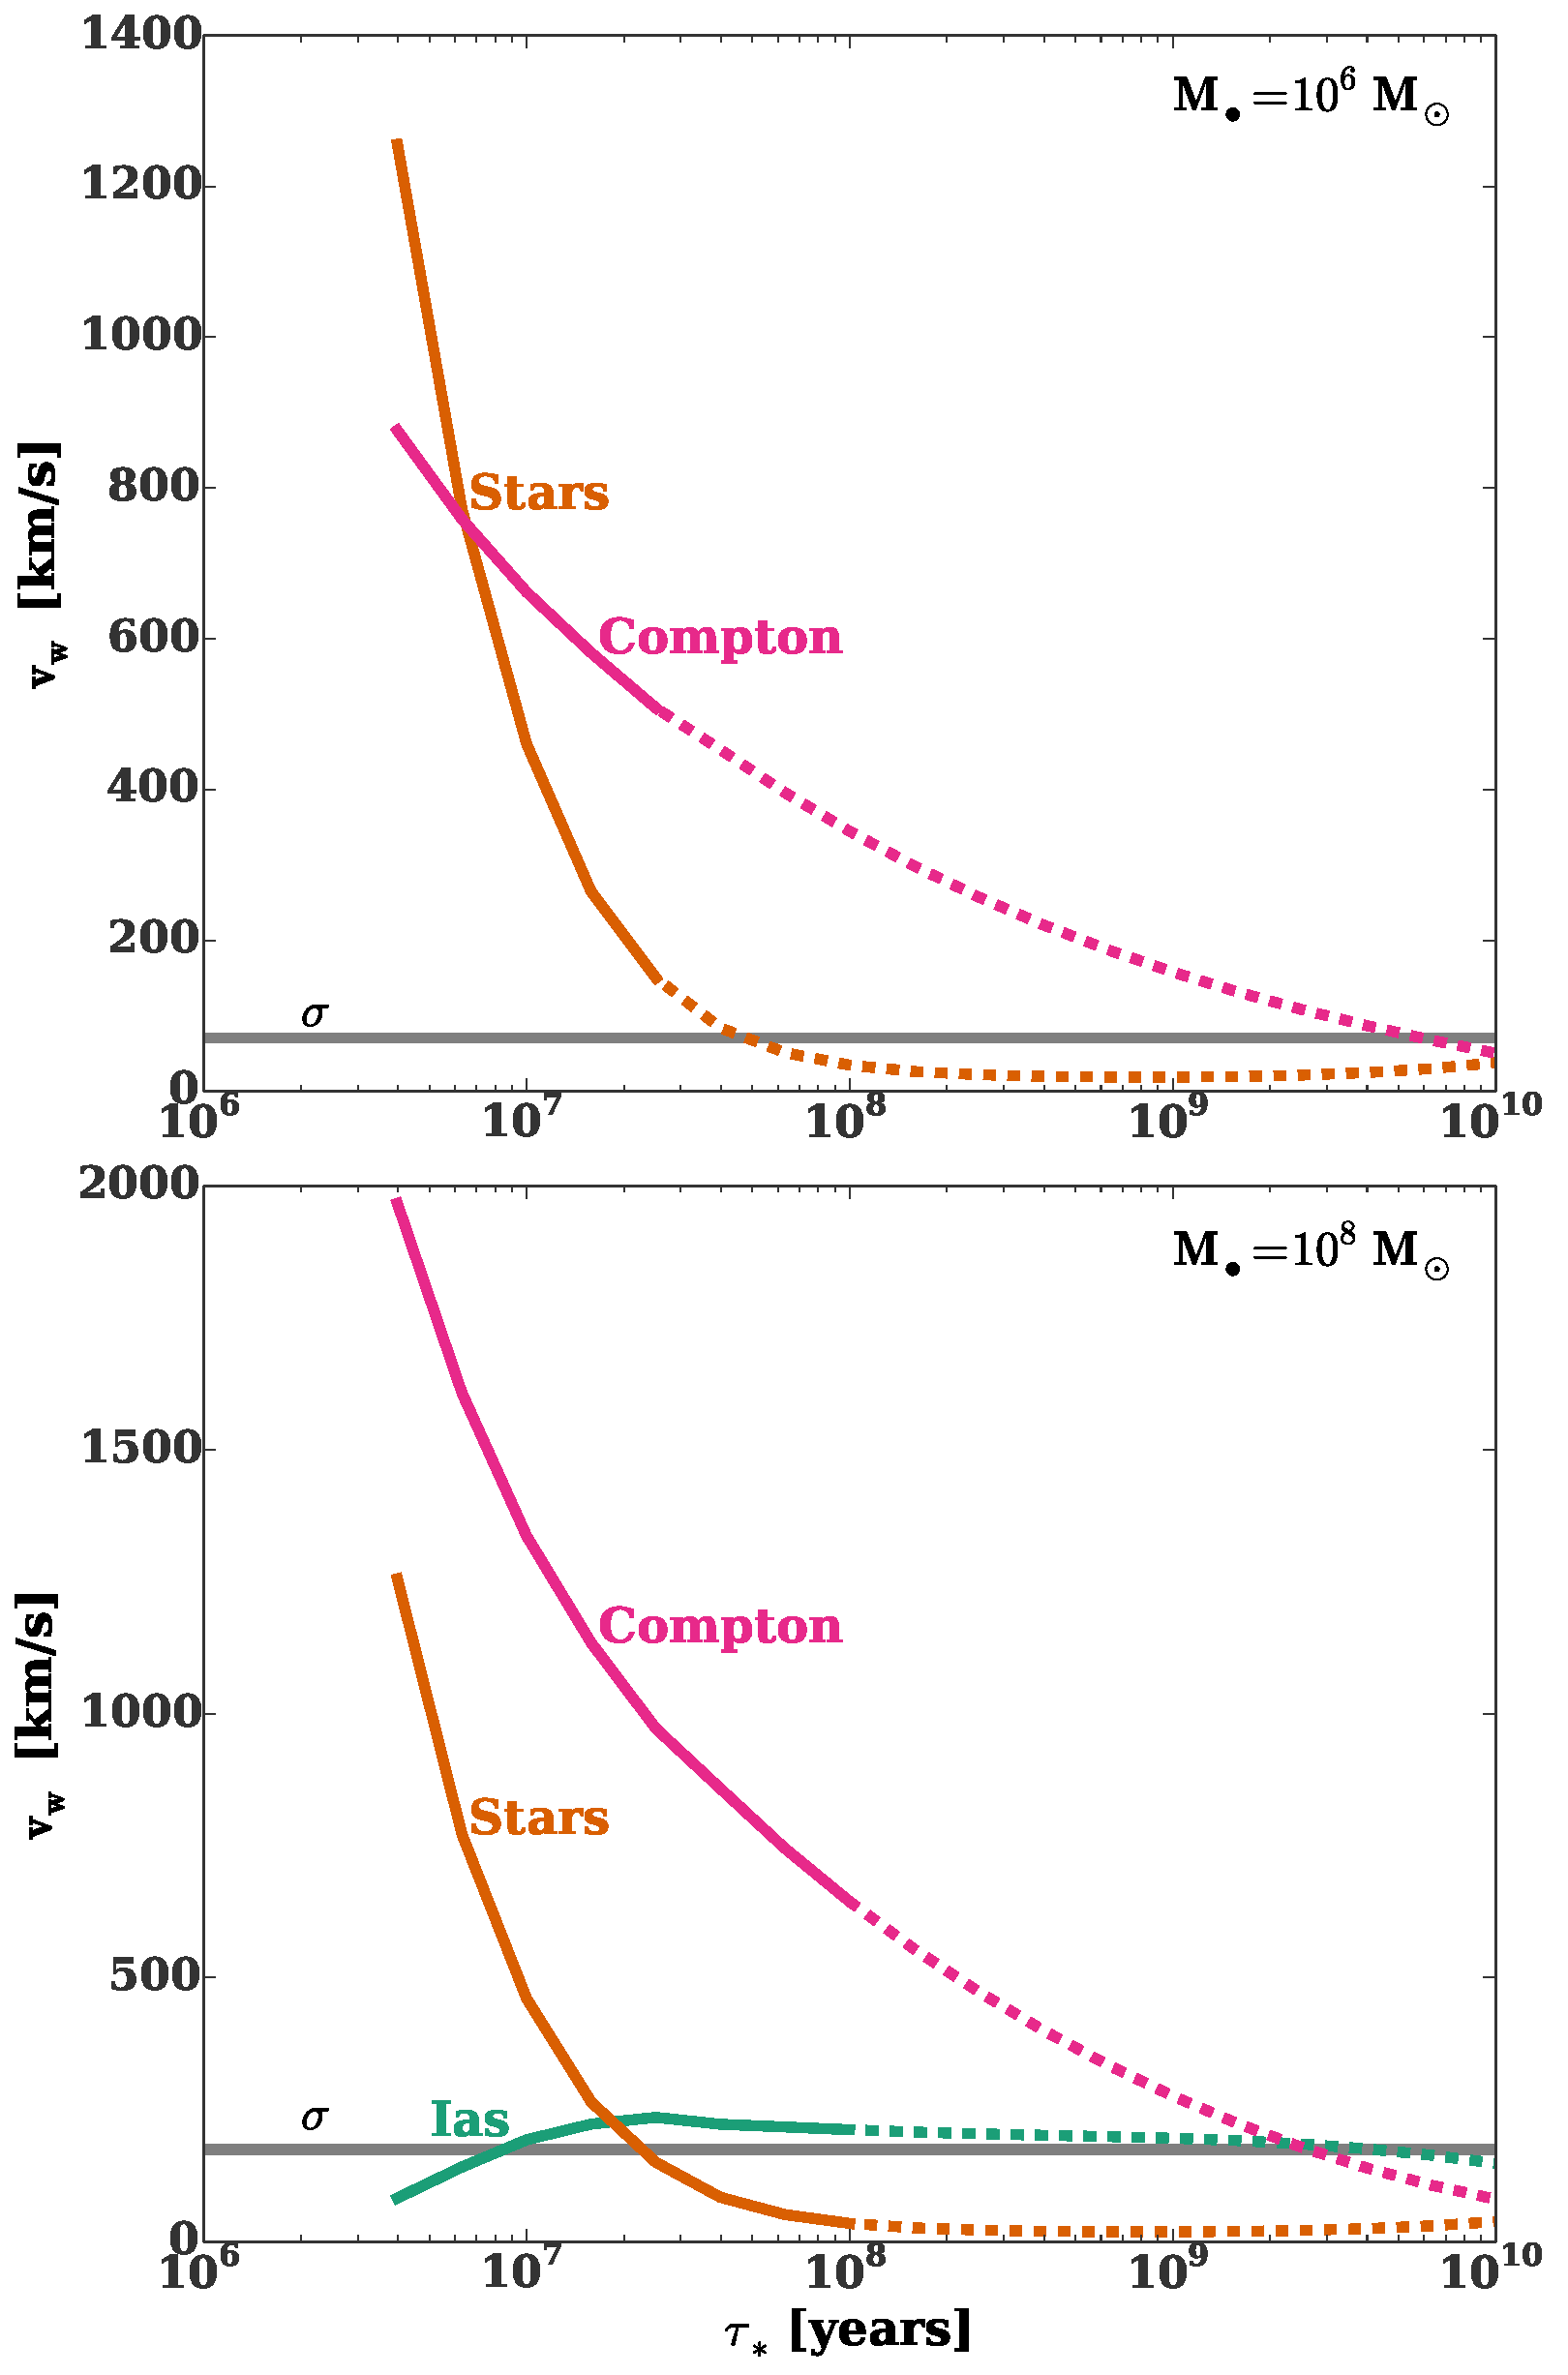
\includegraphics[width=\columnwidth]{vwSourcesImp.pdf}
\caption{\label{fig:vwSourcesImp} Most important sources of heating
  after a burst of star formation for $\Mbh=10^6 \Msun$ (top panel)
  and $\Mbh= 10^8 \Msun$ (bottom panel). We also show the velocity
  dispersion from the $\Mbh-\sigma$ relationship as a horizontal gray line
  \citep{Gultekin+09}.}
\end{figure}


\begin{figure}
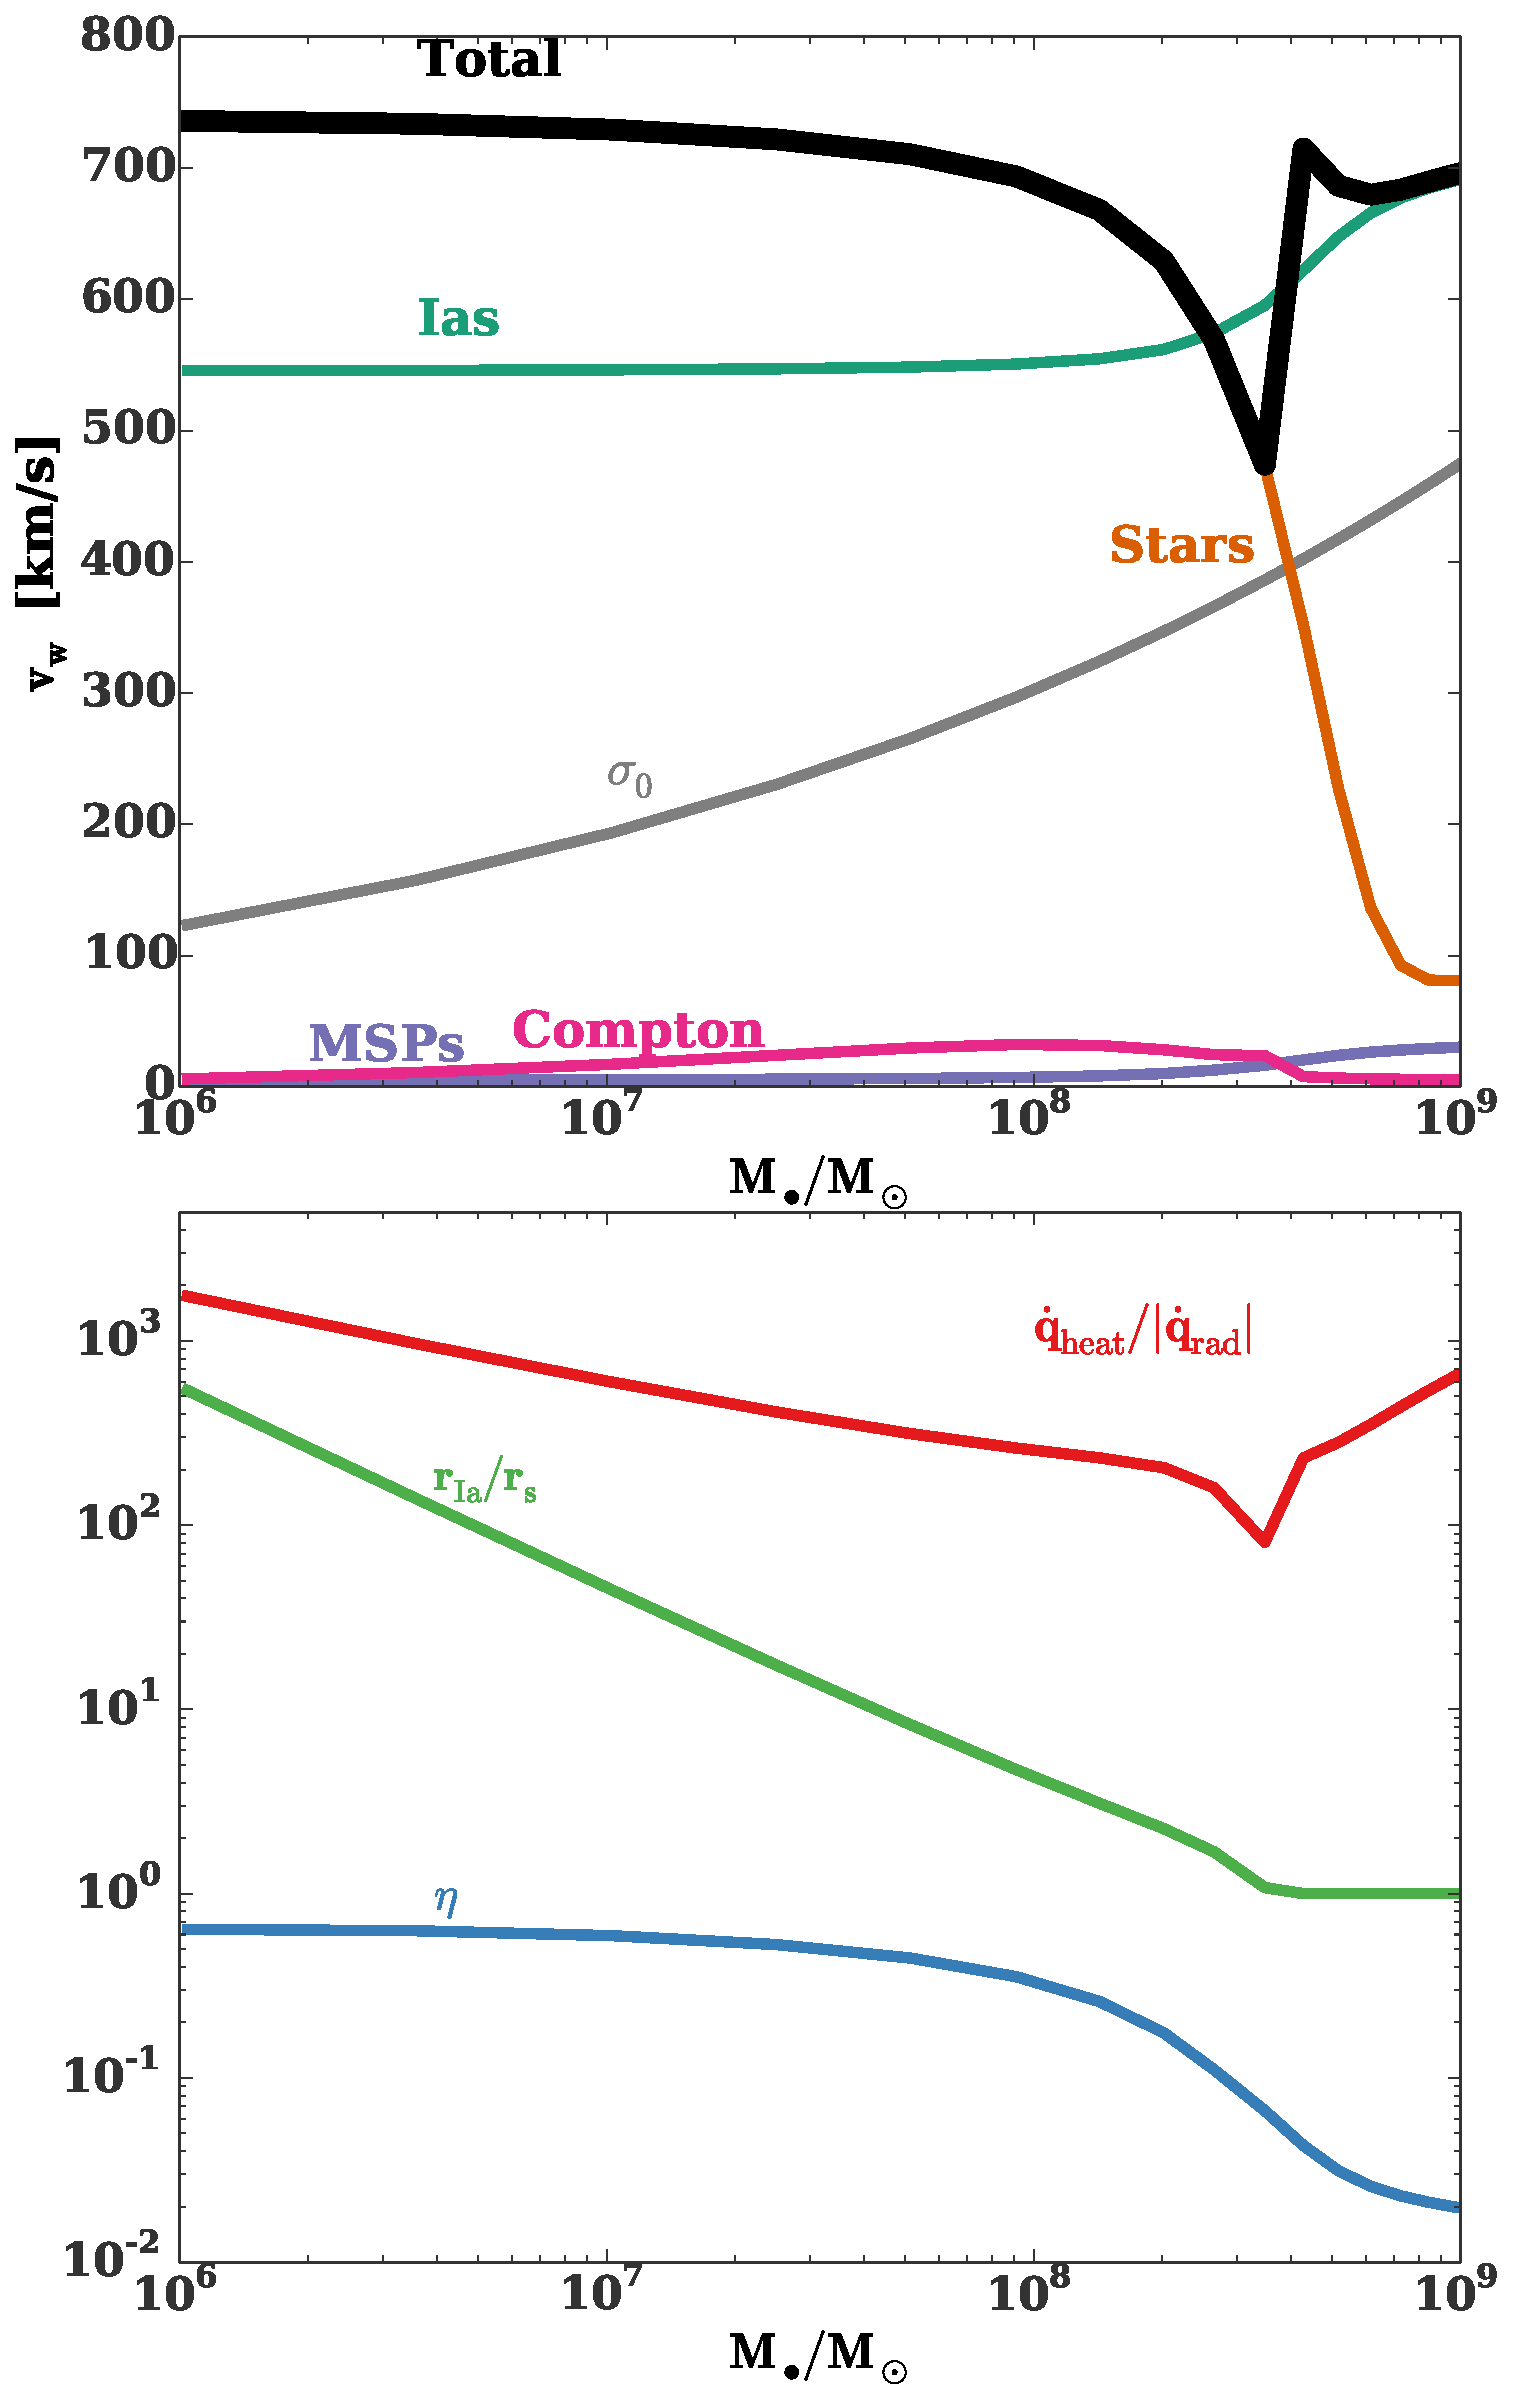
\includegraphics[width=\columnwidth]{vwSources.pdf}
\caption{\label{fig:vwSources} {\emph Top Panel:}Sources contributing
  to the heating rate of the CNM, $\vwO$, including stellar wind
  heating ({\it orange}), Ia supernovae ({\it green}), millisecond
  pulsars ({\it blue}), and compton heating ({\it pink}).  Each heating
  source varies with black hole mass $\Mbh$ due to the different
  average star formation history of galaxies of a given halo mass (see
  Appendix~\ref{app:windheat} for the detailed description). The total
  heating rate is shown in black. To account for the non-steady nature
  of the Ia heating we multiply the Ia heating by $e^{-\rs/\rIa}$, so
  the contribution that the heating contribiution from Ia supernovae
  will be suppressed if the time between successive supernovae is much
  greater than the dynamical time at $\rs$. {\emph Bottom panel} The
  ratio of the heating ($\dot{q}_{\rm heat}$) to the cooling rate
  ($\dot{q}_{\rm cool}$) at $\rs$ from the total heating rate in the
  top panel. Above $\Mbh\simeq 5\times 10^7 \Msun$ $\dot{q}_{\rm
    heat}(\rs)<\dot{q}_{\rm cool}(\rs)$ and a thermal instability
  would arise. The thermally unstable region is marked in red in the
  bottom panel. All curves become dashed in the thermally unstable
  region of parameter space: we expect our model to break down in this
  regime as the steady-state assumption would be violated.}
\end{figure}


\begin{figure}
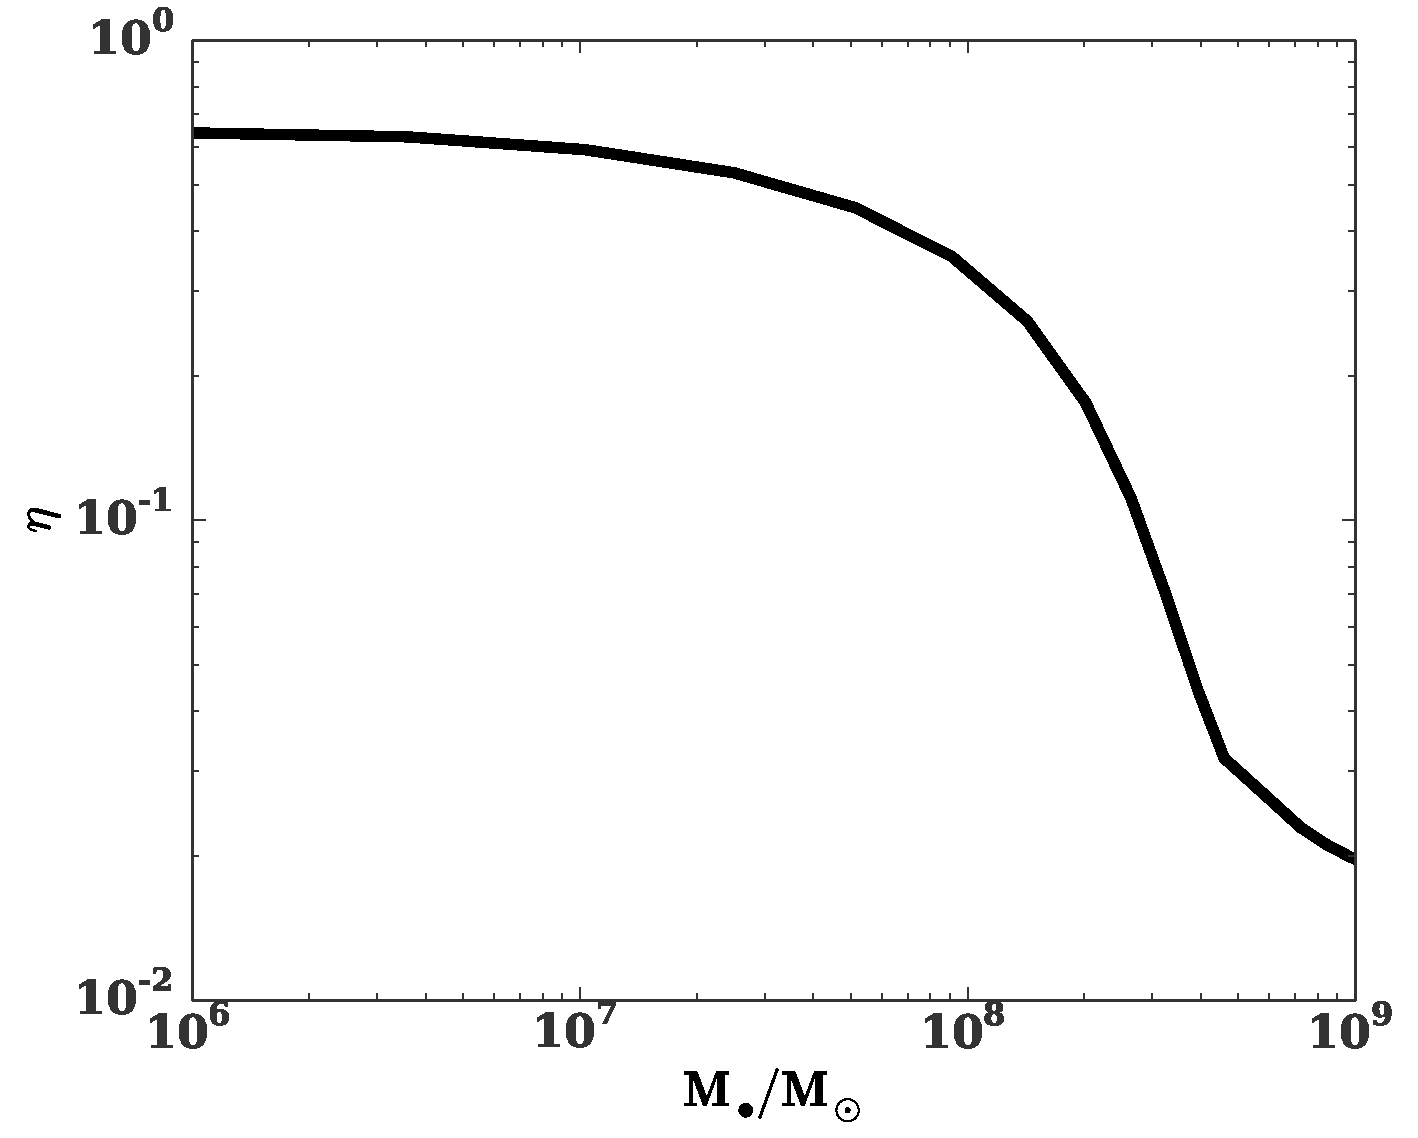
\includegraphics[width=\columnwidth]{eta.pdf}
\caption{\label{fig:eta} Parameter $\eta$ characterizing stellar mass
  loss rate (eq.~[\ref{eq:q}]) as a function of black hole mass
  $\Mbh$, calculated for average star formation histories from
  \citet{MosterNaab+:2013a}  Note that the star
  formation histories in \citet{MosterNaab+:2013a} are in terms of
  halo mass and for each $\Mbh$ we assign the halo mass,
  whose star formation history would produce a bulge consistent with
  the $\Mbh-M_{\rm bulge}$ relationship from
  \citet{McConnellMa:2013a}.}
\end{figure}

The bottom panel of Figure~\ref{fig:vwSources} shows the ratio of
heating to radiative cooling at the stagnation radius
(eq.~[\ref{eq:cooling2}]) as a function of SMBH mass, using our total
heating rate from the top panel Figure \ref{fig:vwSources}.  The
combined heating rate from stellar winds and Compton heating is
insufficient to prevent thermal instability for the high $\Mbh$.
{\bf AG: Should we really be talking about Compton heating stabilizing
the flow}?
% However, if Ia supernovae are included in the schematic way described
% above, the flow again becomes thermally stable for $\Mbh \gtrsim
% XXXX$.


%Although, in principle the Ia contribution to the heating is
%substantial, in practice Ia's occur too infrequently to be a steady
%contribution to the heating rate on small scales (e.g. $r_{\rm Ia} >
%r_{\rm s}$ as shown in Figure~\ref{fig:rs_rIa}). Thus, SNe Ia heating
%by itself would not be able to prevent cooling instability.

% \begin{figure}
% 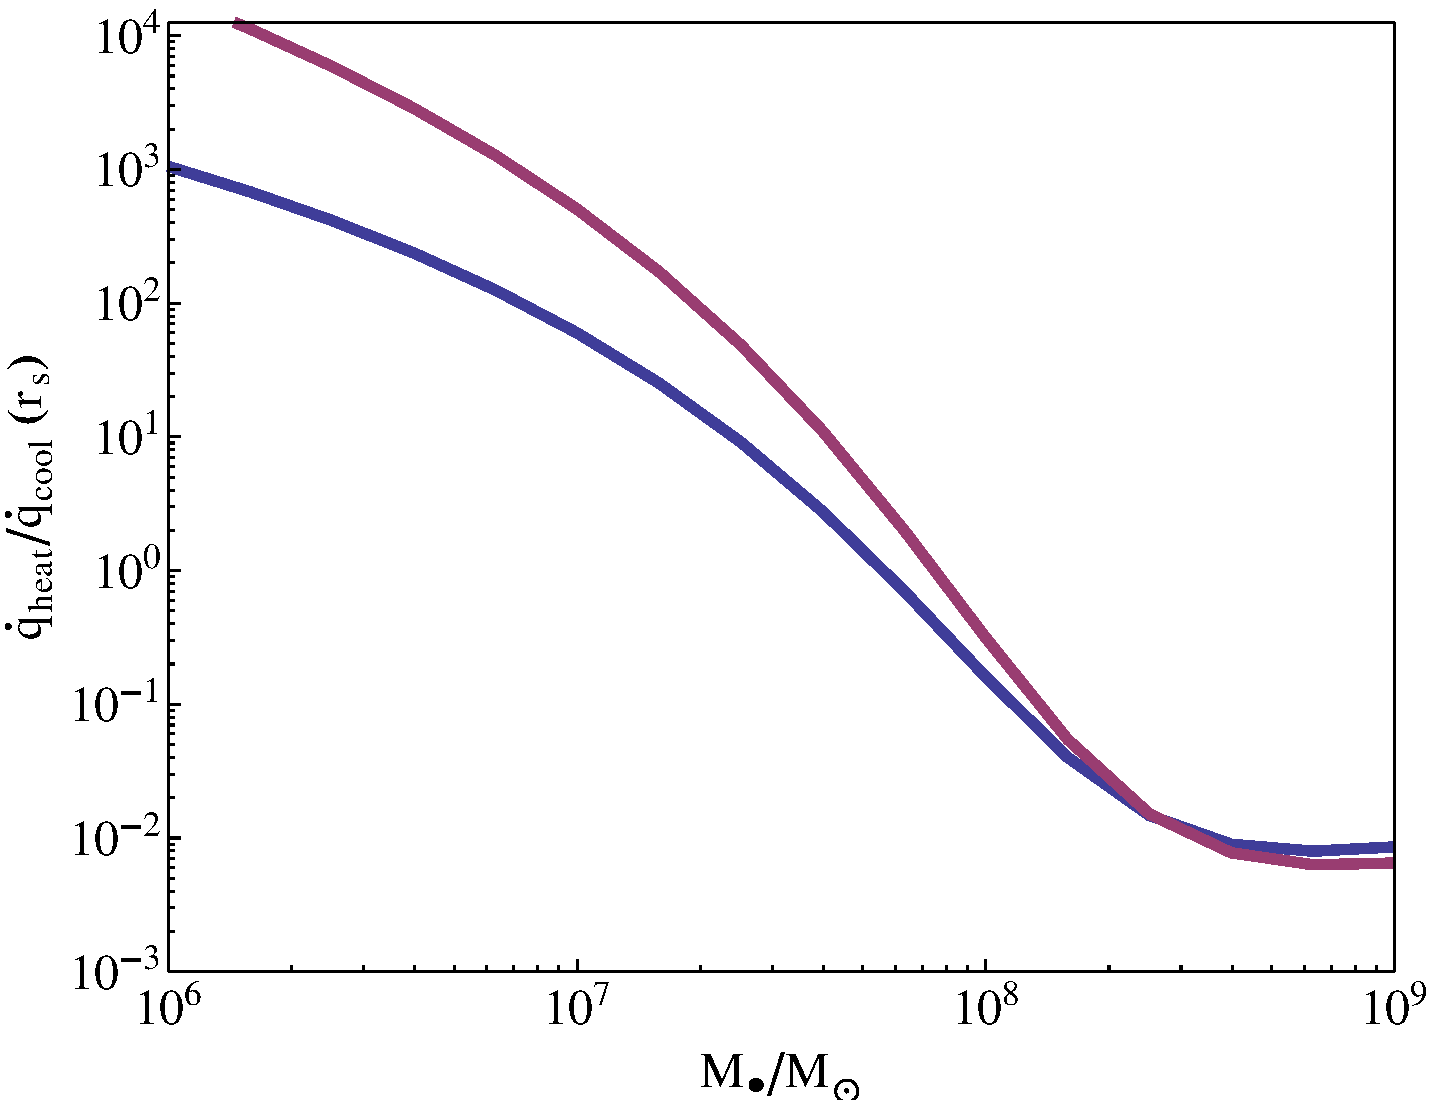
\includegraphics[width=\columnwidth]{cooling2.pdf}
% \caption{\label{fig:cooling2} Ratio of heating rate to cooling rate
%   $\rs$ versus $\Mbh$ for core ($\Gamma=0.1$) galaxies ({\it dashed})
%   and cusp ($\Gamma=0.8$) galaxies ({\it solid}). Ratio is calculated
%   using equation~\eqref{eq:cooling2} and the results for $\vwO$ and
%   $\eta$ in Figures~\ref{fig:vwSources} and~\ref{fig:eta}}
% \end{figure}


\begin{figure}
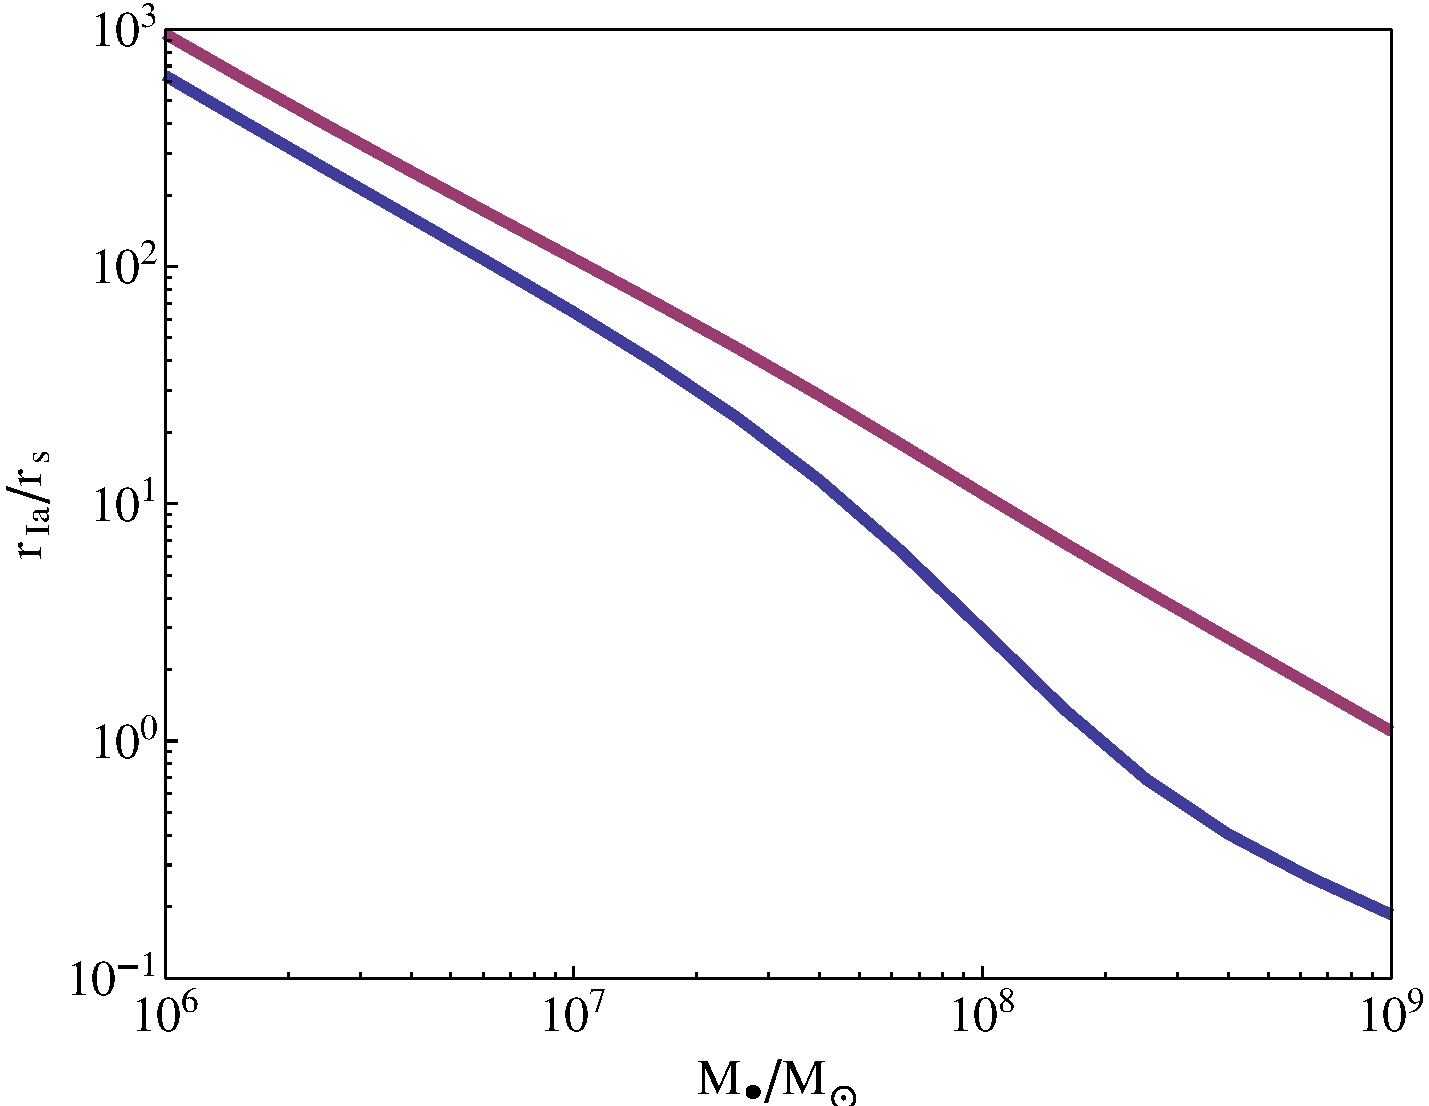
\includegraphics[width=\columnwidth]{rs_rIa.pdf}
\caption{\label{fig:rs_rIa} $\rIa/\rs$ vs. $\Mbh$. $\rIa$ is
  calculated using equation~\eqref{eq:rIa} {\bf AG: I am just
    referring to the first part of the equation here--I use the
    appropriate convolution the Ia rate here}. $\rs$ is calculated
  using the equation~\eqref{eq:stag_simple} and the $\vwO$
  corresponding to each $\Mbh$--see Figure~\ref{fig:vwSources}. For
  the blue curve we use the total $\vwO$ from stars, MSP, and
  black hole feedback (e.g. the solid black curve in
  Figure~\ref{fig:vwSources}).}
\end{figure}

% Figure~\ref{fig:vweff} shows an estimate of how the combined heating
% depends on the age of the stellar population $\tage$ and the SMB mass
% $\Mbh$.  For $M_{\bullet} \gtrsim 1.5\times 10^8 (\tau_{\star}/t_{\rm
%   h})^{0.5} \Msun$, SNe Ia occur sufficiently frequently within the
% stagnation radius (i.e., $r_{\rm Ia} > r_{\rm s}$; eq.~[\ref{eq:rIa}])
% to contribute their full heating rate.  $v_{w}^{\rm Ia} \sim
% 250$ km s$^{-1}$.  On the other hand, for lower mass BHs Ia SNe are
% infrequent, in which case main sequence stars ($v_{w}^{\star}
% \simeq 100-150$ km s$^{-1}$) dominate the heating at most times of
% interest.\footnote{Although SN Ia will still occur surrounding low
%   mass SMBHs, if they are infrequent interior to the radius where the
%   accretion rate is being set, then they will not affect the flow near
%   the SMBH at most epochs.}  For very young stellar populations
% ($\tage \lsim 10^7$ years), $\vwO\simeq 1000$ km s$^{-1}$ due to
% contributions from line driven winds from high mass main sequence
% stars.

 %  \begin{figure}
%     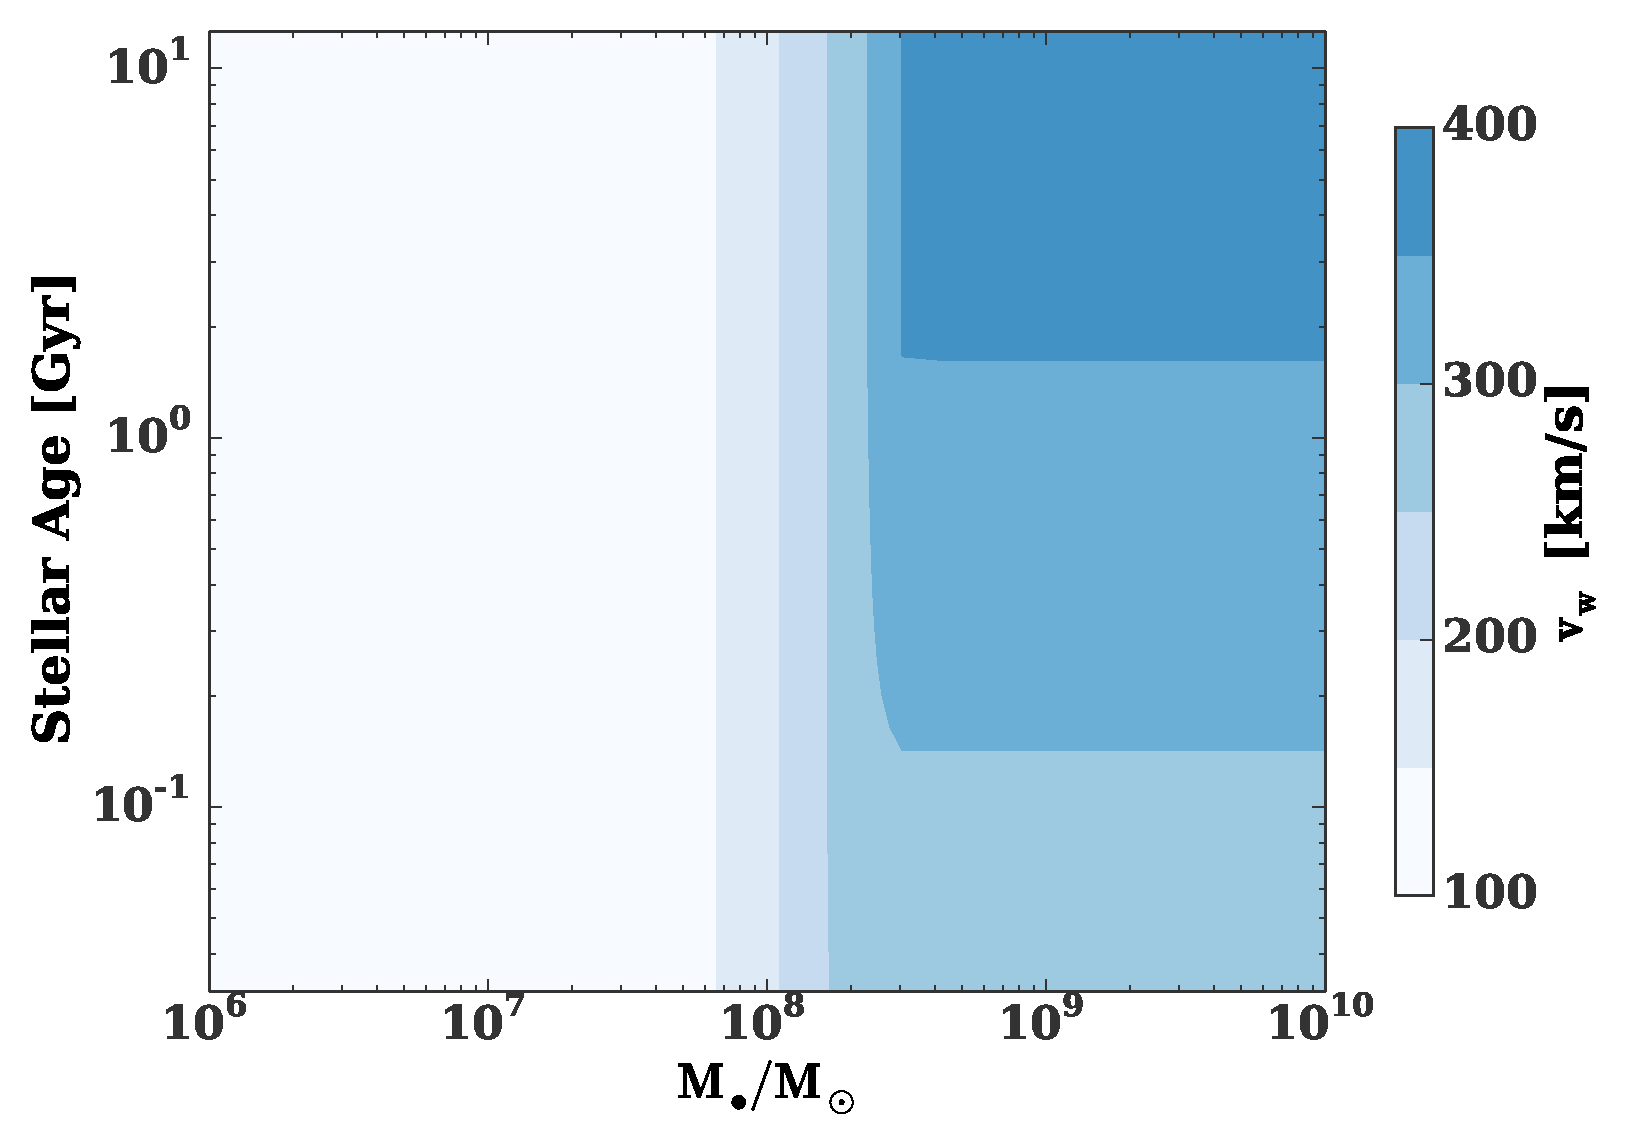
\includegraphics[width=\columnwidth]{vw-contour.eps}
%     \caption{\label{fig:vweff} Combined heating rate $\vwO$ of the CNM
% in the parameter space of SMBH mass $\Mbh$ and age of the stellar
% population $t_{\star}$.  We assume that stellar winds contribute a
% constant heating rate $100$ km/s. The contribution from SNe Ia is
% calculated using equation (\ref{eq:vw_sne}), with thermalization
% efficiency $\epsilon_{\rm Ia}=0.4$. The contribution from SNe Ia is
% only added if the $r_s$ corresponding to the resulting $\vwO$ is
% outside $\rIa$.  {\bf BDM: Correct for dependence of Ia heating on
% time!  among other things}}%describe other cases here.
%   \end{figure}


\section{Applications}
\label{sec:applications}

\subsection{Mass accretion rate}
\label{sec:mdot}

For each solution we calculate the accretion rate $\dot{M}$ onto the
SMBH in units of the Eddington accretion rate $\dot{M}_{\rm edd}
\equiv L_{\rm edd}/0.1 c^{2}$, where $L_{\rm edd} \approx 1.4\times
10^{46}M_{\bullet,8}$ erg s$^{-1}$.  Figure~\ref{fig:mdot_mass} shows
$\dot{M}/\dot{M}_{\rm edd}$ as a function of $\Mbh$ for different
values of $\vwO =$ 300, 600 and 1200 km s$^{-1}$, and for both core
($\Gamma$=0.1) and cusp galaxies ($\Gamma$=0.8).

For fixed wind heating $\dot{M}/\dot{M}_{\rm edd}$ tends to increase
with SMBH mass $\propto M_{\bullet}^{0.5(0.8)}$ for core(cusp)
galaxies, respectively.  This appears to be in contradiction with the
general down sizing trend observed for SMBH accretion in the local
universe (e.g.~\citealt{Heckman+04}; \citealt{Gallo+08}), such as the
fact that for quiescent galaxies the nuclear X-ray luminosity obeys
$L_X \sim \Mbh^\alpha$, where $\alpha\simeq 0.7-0.8$
\citep{Miller+15}.  Our model instead predicts that $\Mdot
\sim \Mbh^{1.5-2}$, such that if $L_x\sim M$, then we would have $\L_x
\sim \Mbh^{1.5-2}$, steeper than the observed relationship.

Figure~\ref{fig:miller} shows our predicted ${\rm L_{X}/L_{edd}}$ for
core (blue) and cusp (green) galaxies superimposed with x-ray
measurements (red stars), upper limits (red triangles) from
\citet{Miller+15}.  For our theoretical predictions $L_X=\epsilon
\Mdot c^2$, where $\epsilon$ is and efficiency factor and $\Mdot$ is
calculated using Equation~\eqref{eq:mdot_analytic}, with the value of
the wind heating parameter, $\vw$, and the mass return parameter,
$\eta$ set by the average star formation history for each $\Mbh$ (see
the black lines in Figures~\ref{fig:vwSources} and~\ref{fig:eta}). We
try two different prescriptions for $\epsilon$: 
$\epsilon=10^{-4}$ in the left-hand panel and $\epsilon=10^{-1}
\Mdot/0.01 \MdotEdd$ right-hand panel.  

\begin{figure*}
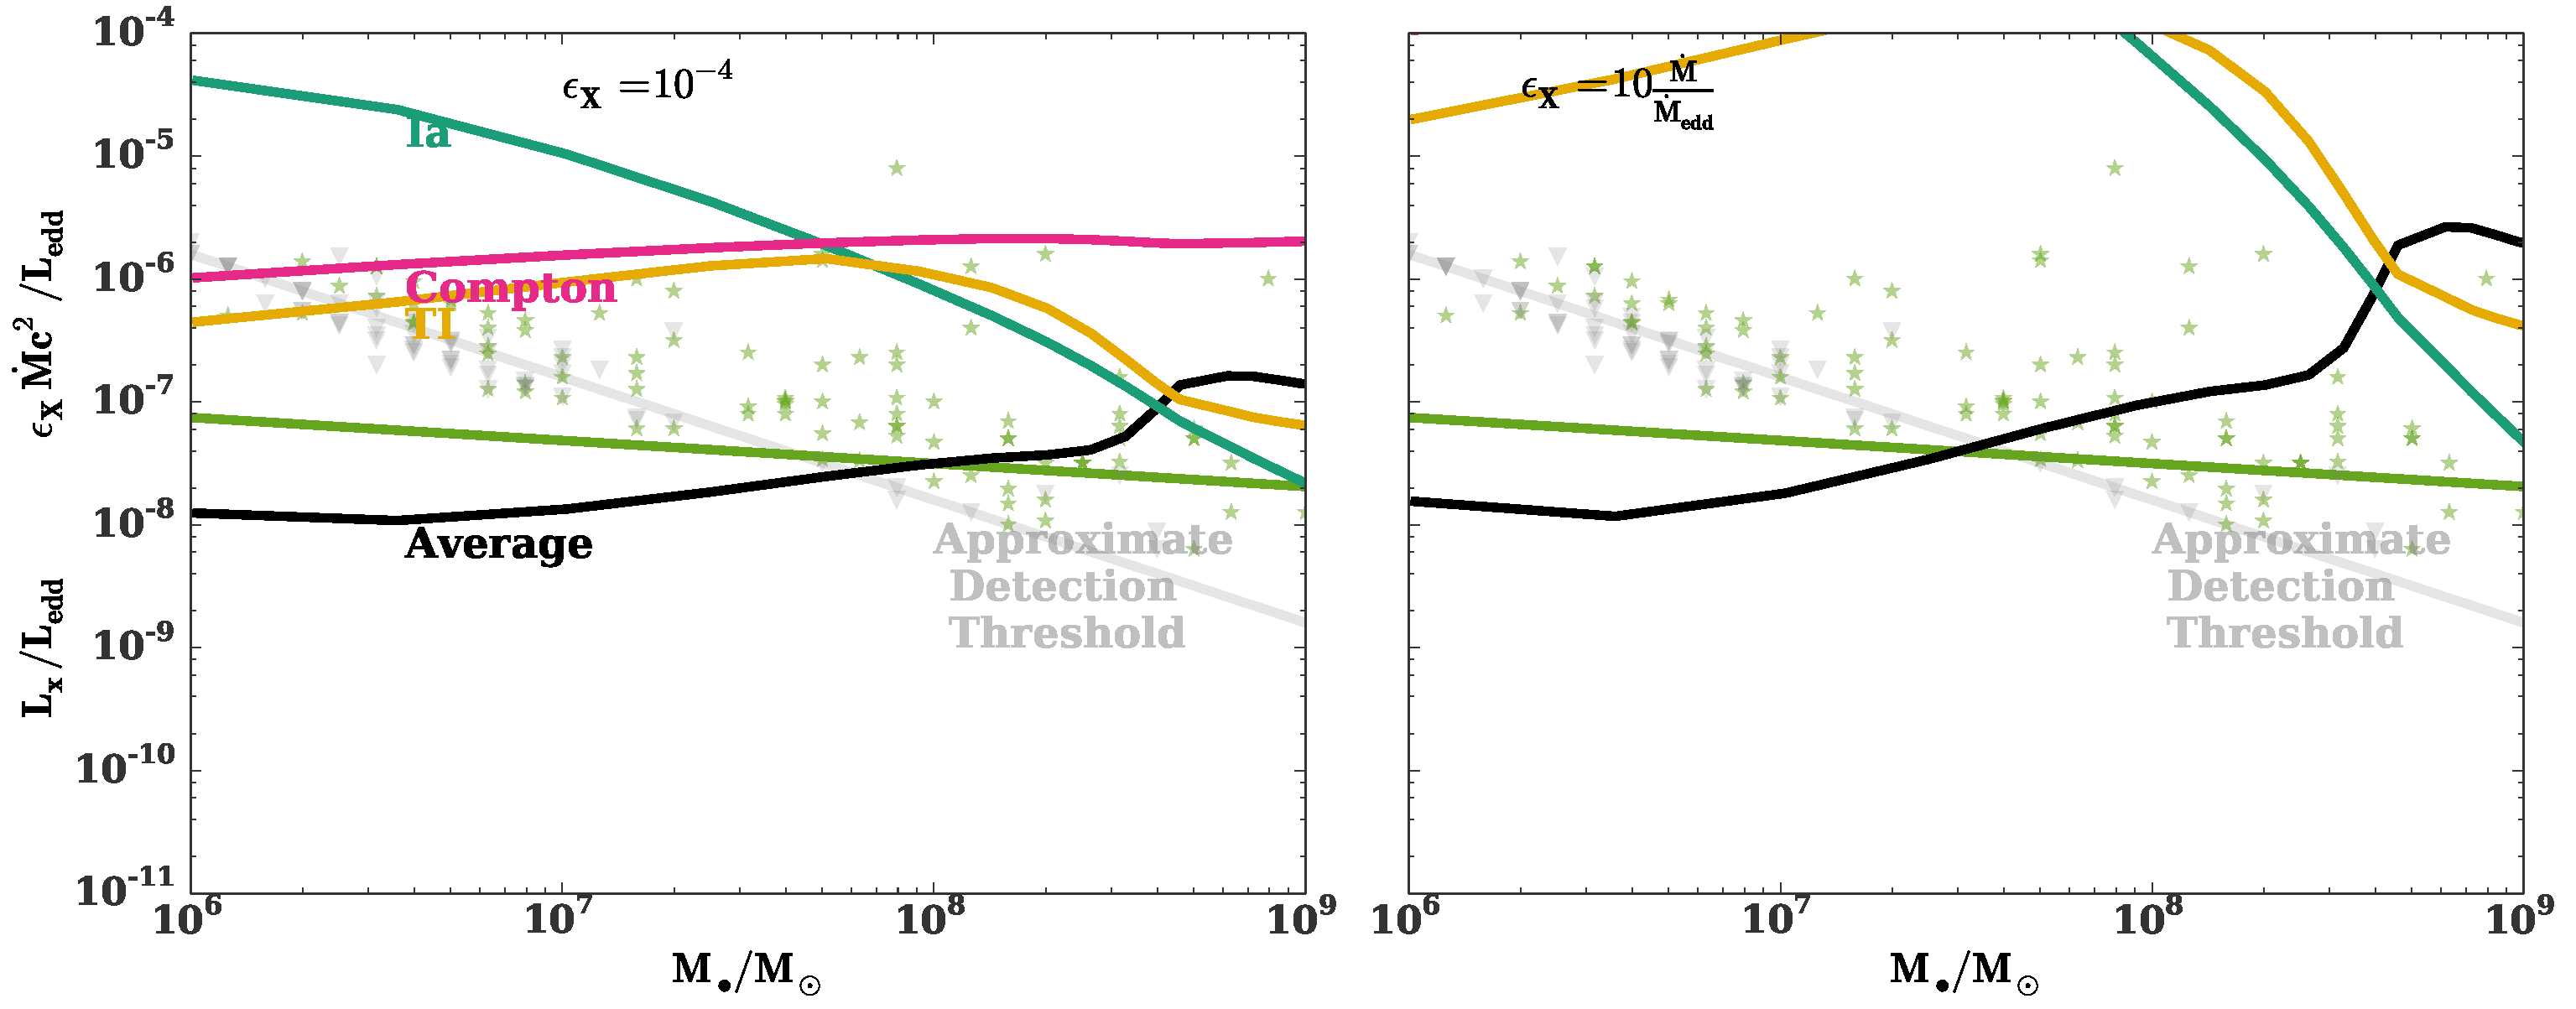
\includegraphics[width=\textwidth]{miller.pdf}
\caption{\label{fig:miller} $\epsilon_X \Mdot c^2/L_{\rm edd}$ predicted
  from our models compared to $L_X/L_{\rm edd}$ values (red stars) and
  upper limits (red triangles) from \citet{Miller+15}.
  $\epsilon_X=10^{-4}$ in the left-hand panel and $\epsilon_X=0.1
  \frac{\Mdot}{0.01 \MdotEdd}$ in the right-hand panel. The green and
  blue curves represent our predictions for core ($\Gamma=0.1$)
  and cusp ($\Gamma=0.8$) galaxies respectively. They are calculated
  from equation~\eqref{eq:mdot_analytic}, with the wind heating
  parameter, $v_w$ and mass return parameter, $\eta$, corresponding to
  the the average star formation histories in
  \citet{MosterNaab+:2013a} (the black lines in
  Figures~\ref{fig:vwSources} and~\ref{fig:eta}--see
  Appendix~\ref{app:windheat} for a detailed description).
  We also show upper limits $\epsilon_X \Mdot c^2/L_{\rm edd}$ from
  thermal stability (purple) and Ia supernovae (orange).}
\end{figure*}

% Hower, the mass accretion rate is also a sensitive function of the assumed heating rate, such that $\dot{M}\sim\vwO^{-3.8(-2.4)}$ for a core(cusp) galaxies, respectively.  Thus, only a weak positive dependence of $v_{w} \propto M_{\bullet}^{0.25-0.3}$ would be sufficient to explain the trend in X-ray luminosity with BH masses in scenarios where $L_X \propto \dot{M}$, or a somewhat steeper dependence $v_{w} \propto M_{\bullet}^{0.35-0.45}$ if $L_{X} \propto \dot{M}^{2}$.  What could cause this dependence?  Maybe Ia SNa...

% This is shown in the top panel Figure~\ref{fig:bh_xray}. The
% relationship from \citealt{Miller+15} and their detection
% upper limits are the black and blue solid lines
% respectively. The points correspond to the $\dot{M} c^2$ for our
% solutions (scaled by $5\times 10^{-7}$).  We must choose a $\vwO$ for
% each galaxy.  We select $\vwO$=200 km/s, roughly the expected level of
% heating expected from main sequence the stellar winds and MSPs. If
% $L_x \sim \Mdot^2$ the discrepancy becomes worse, as shown in the
% bottom panel of Fig.~\ref{fig:bh_xray}, where we plot $2 \times
% 10^{-4} (\eddr) \Mdot c^2$ from our solutions with the relation from
% \citealt{Miller+15}.


% One possible solution that the wind mass loss rate $\eta$ increases
% with $\Mbh$, as would be expected if low mass SMBH preferentially
% hosted younger stellar populations.  Another possible explanation is
% that the effective heating rate of the CNM $v_{w}$ decreases
% with decreasing SMBH mass.  This could again be due to an older
% stellar population, since $v_{w} \propto \eta^{-1/2}$ for heating
% sources such as SN Ia and millisecond pulsars.
% {\bf AG given our new results on stellar wind heating as a function of
% Mbh. It seems like the first statement is indeed true but I suspect
% vwO actually increases for low Mbh and that this effect actually dominates.}
%, or it could be due to the fact that Ia occur too infrequently inside
%the stagnation radius for low mass black holes.
%AG-We now think that SNe Ia would become important only at the
%highest values of Mbh.
%AG-Note sure where the best place for this discussion would
%be--here or after presenting the comparisons with Miller et al.

\begin{figure}
  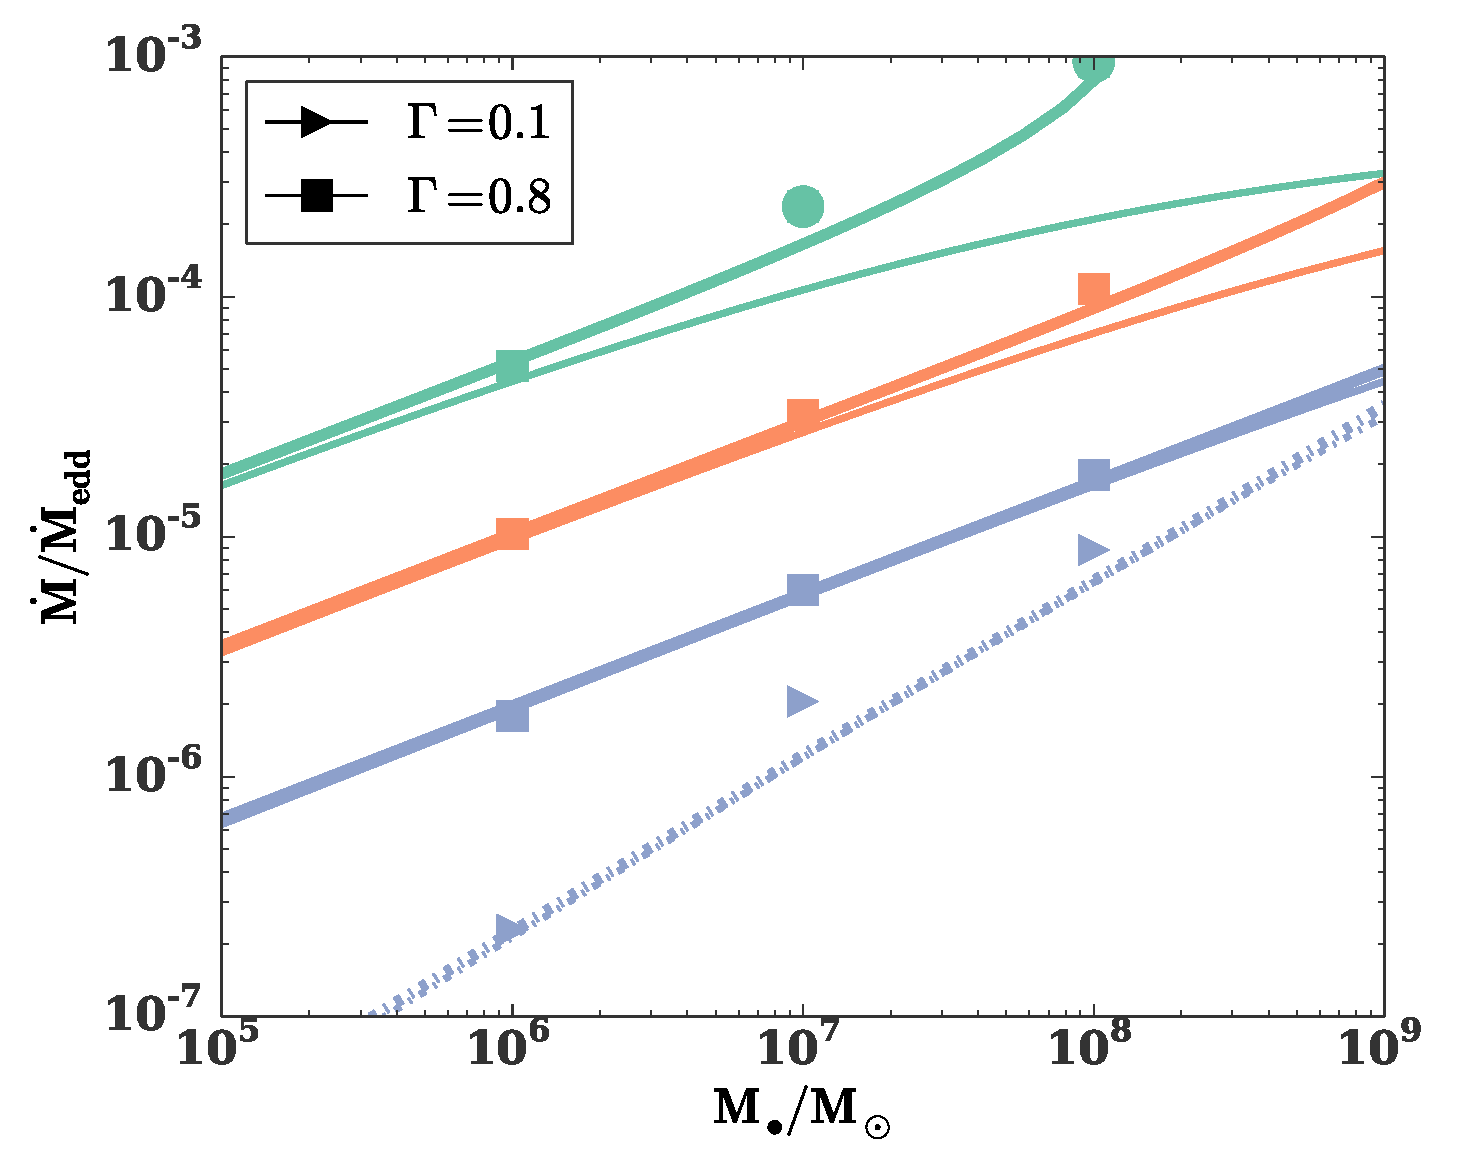
\includegraphics[width=\columnwidth]{mdot_mass.eps}
  \caption{\label{fig:mdot_mass} Accretion rate $\dot{M}$ in units of
    the Eddington rate $\dot{M}_{\rm edd}$ as a function of SMBH mass
    for each galaxy in our sample, calculated for different values of
    the wind heating parameter $\vwO =$ 300 km s$^{-1}$ ({\it green}),
    600 km s$^{-1}$ ({\it orange}), and 1200 km s$^{-1}$ ({\it blue}).
    Squares correspond to cusp galaxies ($\Gamma=0.8$), while
    triangles correspond to cores ($\Gamma$=0.1). The curves correspond
    to the analytic results for $\eddr$ from equation
    (\ref{eq:eddr_analytic}) for cusps (solid lines) and cores (dashed
    lines).  }
\end{figure}

%% AG:  Also want to include a plot of x-ray luminosity (less abstract than the accretion rate). 

\subsection{Comparison to Observations}
{\bf AG: I do want some discussion of reproducing the density profiles
for individual observations, but I am not sure how to do it with our
new gridded approach.}
% \subsubsection{Comparison to measured temperature and density profiles}
% \citet{AllenDunn+:2006a} use {\it Chandra} X-ray observations to infer the radial temperature and density profiles in the nuclei of nine nearby X-ray luminous elliptical galaxies.  \citet{RussellMcNamara+:2013a} performed a similar analysis with a somewhat enlarged galaxy sample.  Interestingly, these works find a correlation between the accretion rate inferred assuming Bondi accretion and the AGN jet power, which is estimated by the PdV work required to inflate observed cavities in the X-ray emitting gas.  
% % At some point it would be useful to describe the differences between
% % these two sets of observations \citealt{RussellMcNamara+:2013a}
% % tries several different extrapolation schemes for the gas density,
% % and finds that that the uncertainty in extrapolating the density
% % profile is the dominant source of uncertainty in measuring the
% % accretion rate. Find total number which overlaps once the Russell
% % galaxies are included...

% Five of the galaxies in the \citet{AllenDunn+:2006a} sample overlap with that in \citetalias{WangMerritt:2004a}.  We may thus compare our results for the $T$ and $\rho$ profiles with those inferred from observations for the overlapping galaxies.  The results of this exercise are presented in Fig.~\ref{fig:allen_compare}.

% Note that we have two free parameters ($\eta$ and $\vwO$) in our
% model, which implies that we can always match the observed temperature
% and densities at at least one point.  As a general rule, we find that
% a wind heating parameter $\vwO=500$ km s$^{-1}$ gives rough agreement
% with the observed temperatures.  We now highlight results for specific
% galaxies.
% % Thus, we choose $\vwO=500$ km/s.  We choose an
% % $\eta$ so that our solution would be consistent with the observed
% % density profiles. The comparison is shown in
% %% AG-The chosen properties, in particular eta may be summarized in a tabe.
% %% AG-Mention rising temperature profiles on large scales.

% \begin{itemize}
% % \item \emph{NGC4486} %eta=0.2
% %   On scales of $\sim1$ kpc the density profile in
% %   \citealt{AllenDunn+:2006a} is shallower than in our model. Our model
% %   has a break in the gas density at $\sim 300$ pc--near the location
% %   of the Nuker break radius for this galaxy at 560 pc. There is an
% %   observed break in the density, but on a scale of a few kpc.

% %   The temperature is assumed to be flat from the resolution limit
% %   inwards in \citealt{AllenDunn+:2006a}. However, in our models $T$
% %   increases monotonically towards the galactic center. This increase
% %   is due to the increased velocity dispersion (and thus increased
% %   heating) towards the galactic center.

% \item \emph{NGC5813} %eta=0.1 
%   The observed density profile (\citealt{RussellMcNamara+:2013a}) is
%   shallower than our calculated density profile, which has a sharp
%   break at $\sim$0.1 kpc, the location of the break radius in the
%   Nuker profile (this is the radius where the stellar light profile
%   transitions from a shallower inner power law slope to a steeper
%   outer power law slope).

%   For this galaxy we found that we could reproduce the observed
%   temperature on large scales with $\vwO=500$ km/s. The increased
%   velocity disperision towards the galactic center results in a sharp
%   increase in $T$ at small radii, which is not captured in the
%   observations due to resolution issues.
% \end{itemize}

% %It would be nice to have error bars for the observational points in this plot...
% \begin{figure*}
%   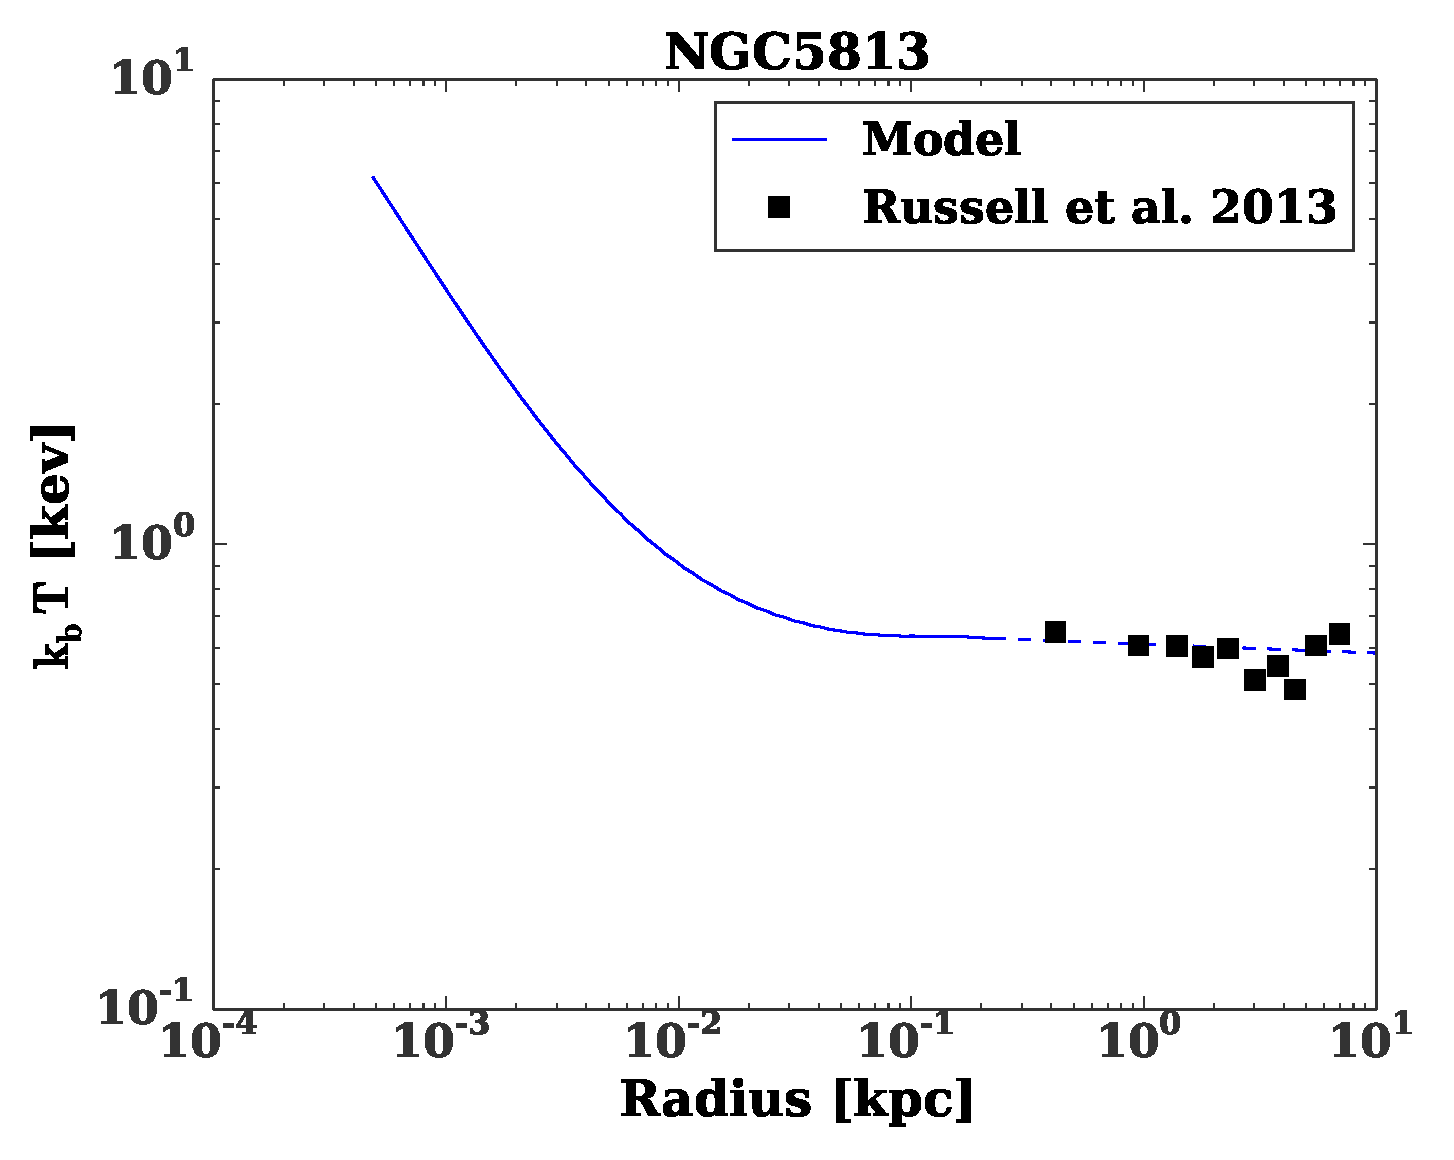
\includegraphics[width=\columnwidth]{NGC5813_T.eps}
%   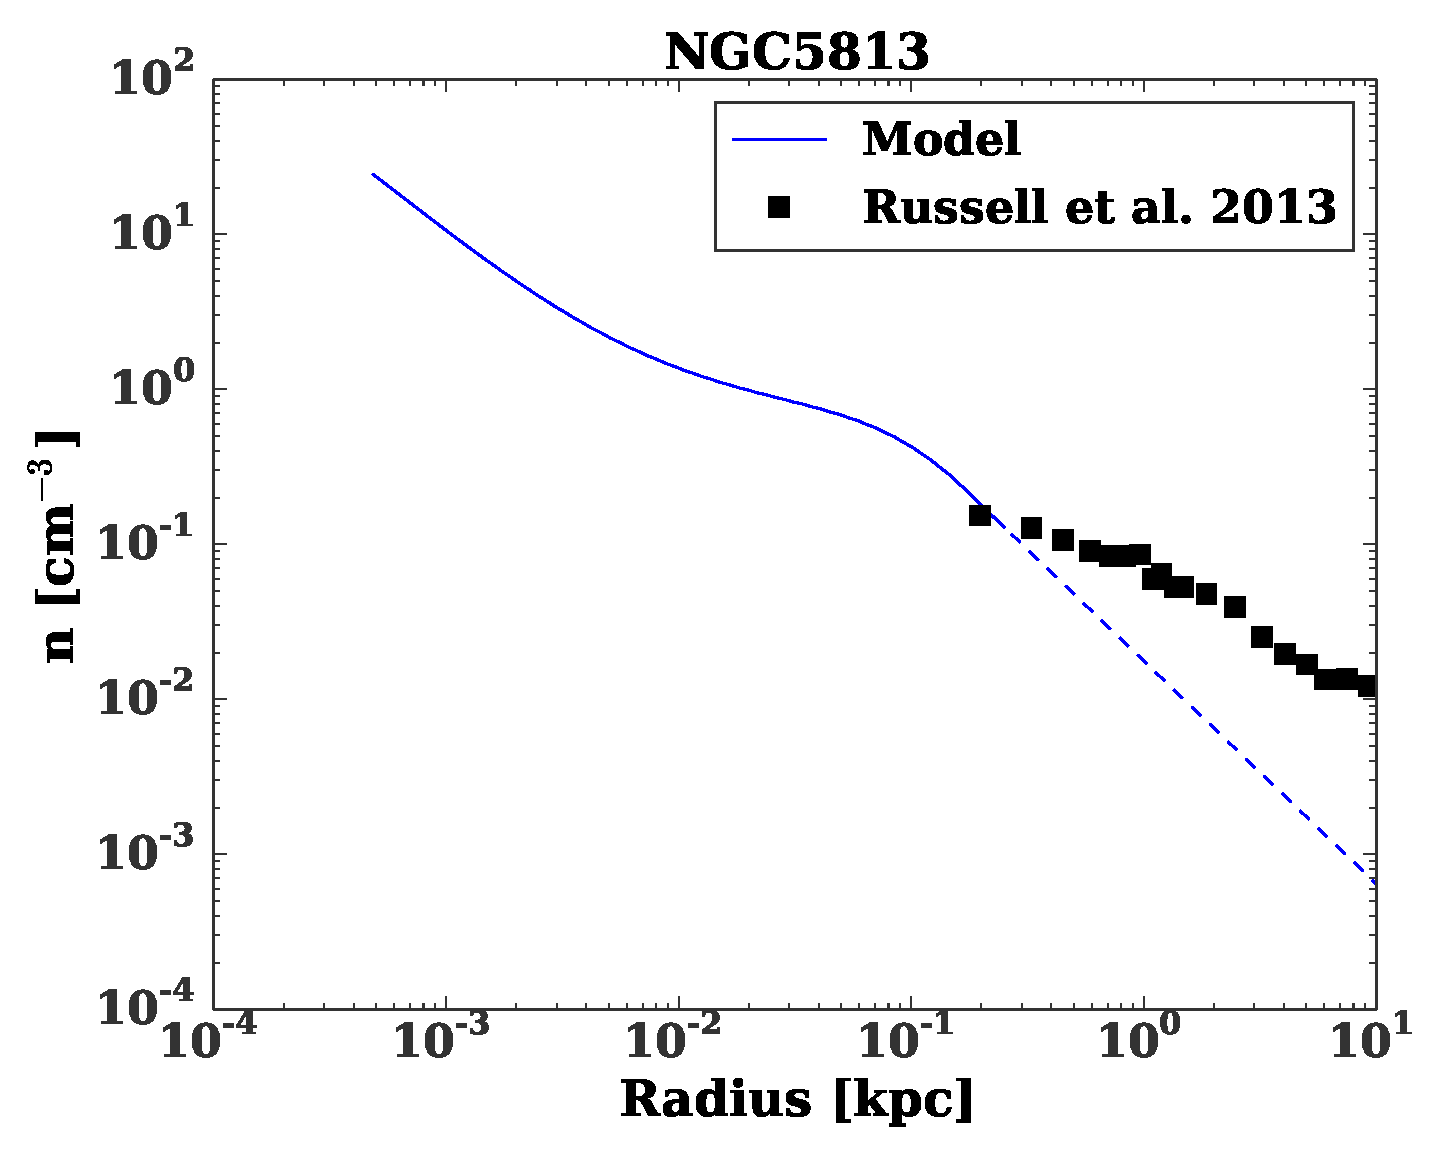
\includegraphics[width=\columnwidth]{NGC5813_rho.eps}
%   \caption{\label{fig:allen_compare} Comparison of the radial profiles
%     (blue lines) of electron number density $n_e$ and temperature $T$
%     to the measured values (black square) in \citet{AllenDunn+:2006a}
%     and \citet{ RussellMcNamara+:2013a}. The dashed blue lines are
%     power law extrapolations of our profiles. Note that in going from
%     $\rho$ to $n_e$ we our adopted value for the molecular weight $\mu=1$.}
%   %% AG in the future we will have to be carfeful of the mean molecular weight.
% \end{figure*}

% \subsubsection{Comparison with observed X-ray Luminosity-Mass
%   Relation}
% %Note currently I reverse-engineer the stellar mass from the black
% %hole mass inferred from M-sigma; however, it would be better to use
% %the tabulated black hole mass from the Mbh-Mbulge relation.
% Fig. 1 of \citealt{Miller+15} plots the observed
% relationship of unresolved x-ray luminosity versus galactic stellar
% mass for a sample of quiescent galaxies. We may construct a similar
% relationship with our own sample using the inferred accretion rates
% from our solutions.  To infer an x-ray luminosity for each solution,
% we scale our calculated $\Mdot c^2$ by a constant. We pick $5\times
% 10^{-7}$, which gives x-ray luminosities comparable to
% those in \citealt{Miller+15}. We also try an alternate
% prescription in which $L_x$ is quadratic in $\Mdot$. In particular, we
% take $L_x=2 \times 10^{-4} (\eddr) \Mdot c^2$. 

% We must make choose a $\vwO$ for each galaxy.  We select $\vwO$=200
% km/s if $\rs<\rIa$ for this solution, $\vwO$=500 km/s if $\rs>\rIa$
% for this solution, or exclude it.  At low $\Mbh$ we have $\vwO$=200
% km/s and at high $\Mbh$ we have $\vwO$=500 km/s.  Note that much of
% our sample is excluded in this Fig., since for $\vwO$=200 km/s we
% would have $\rs>\rIa$ and four $\vwO$=500 km/s we would have
% $\rs<\rIa$ (i.e. the relative locations of $\rs$ and $\rIa$ would be
% inconsistent with the assumed level of heating).

% %AG-power law may be closer to 1.4 & 1.8 than to 1.5 & 2.
% Our results are plotted in Fig.~\ref{fig:bh_xray}. In our model
% there is a steeper dependence $\Mbh$ on $M_{\rm gal}$ than in
% \citealt{Miller+15}. We find $L_x \propto M_{\rm gal}^{1.5}$ when
% $L_x \propto M_{\rm gal}^{2}$, whereas \citealt{Miller+15} finds
% that $L_x \propto M_{\rm gal}^{0.7-0.8}$. 

% \begin{figure}
% 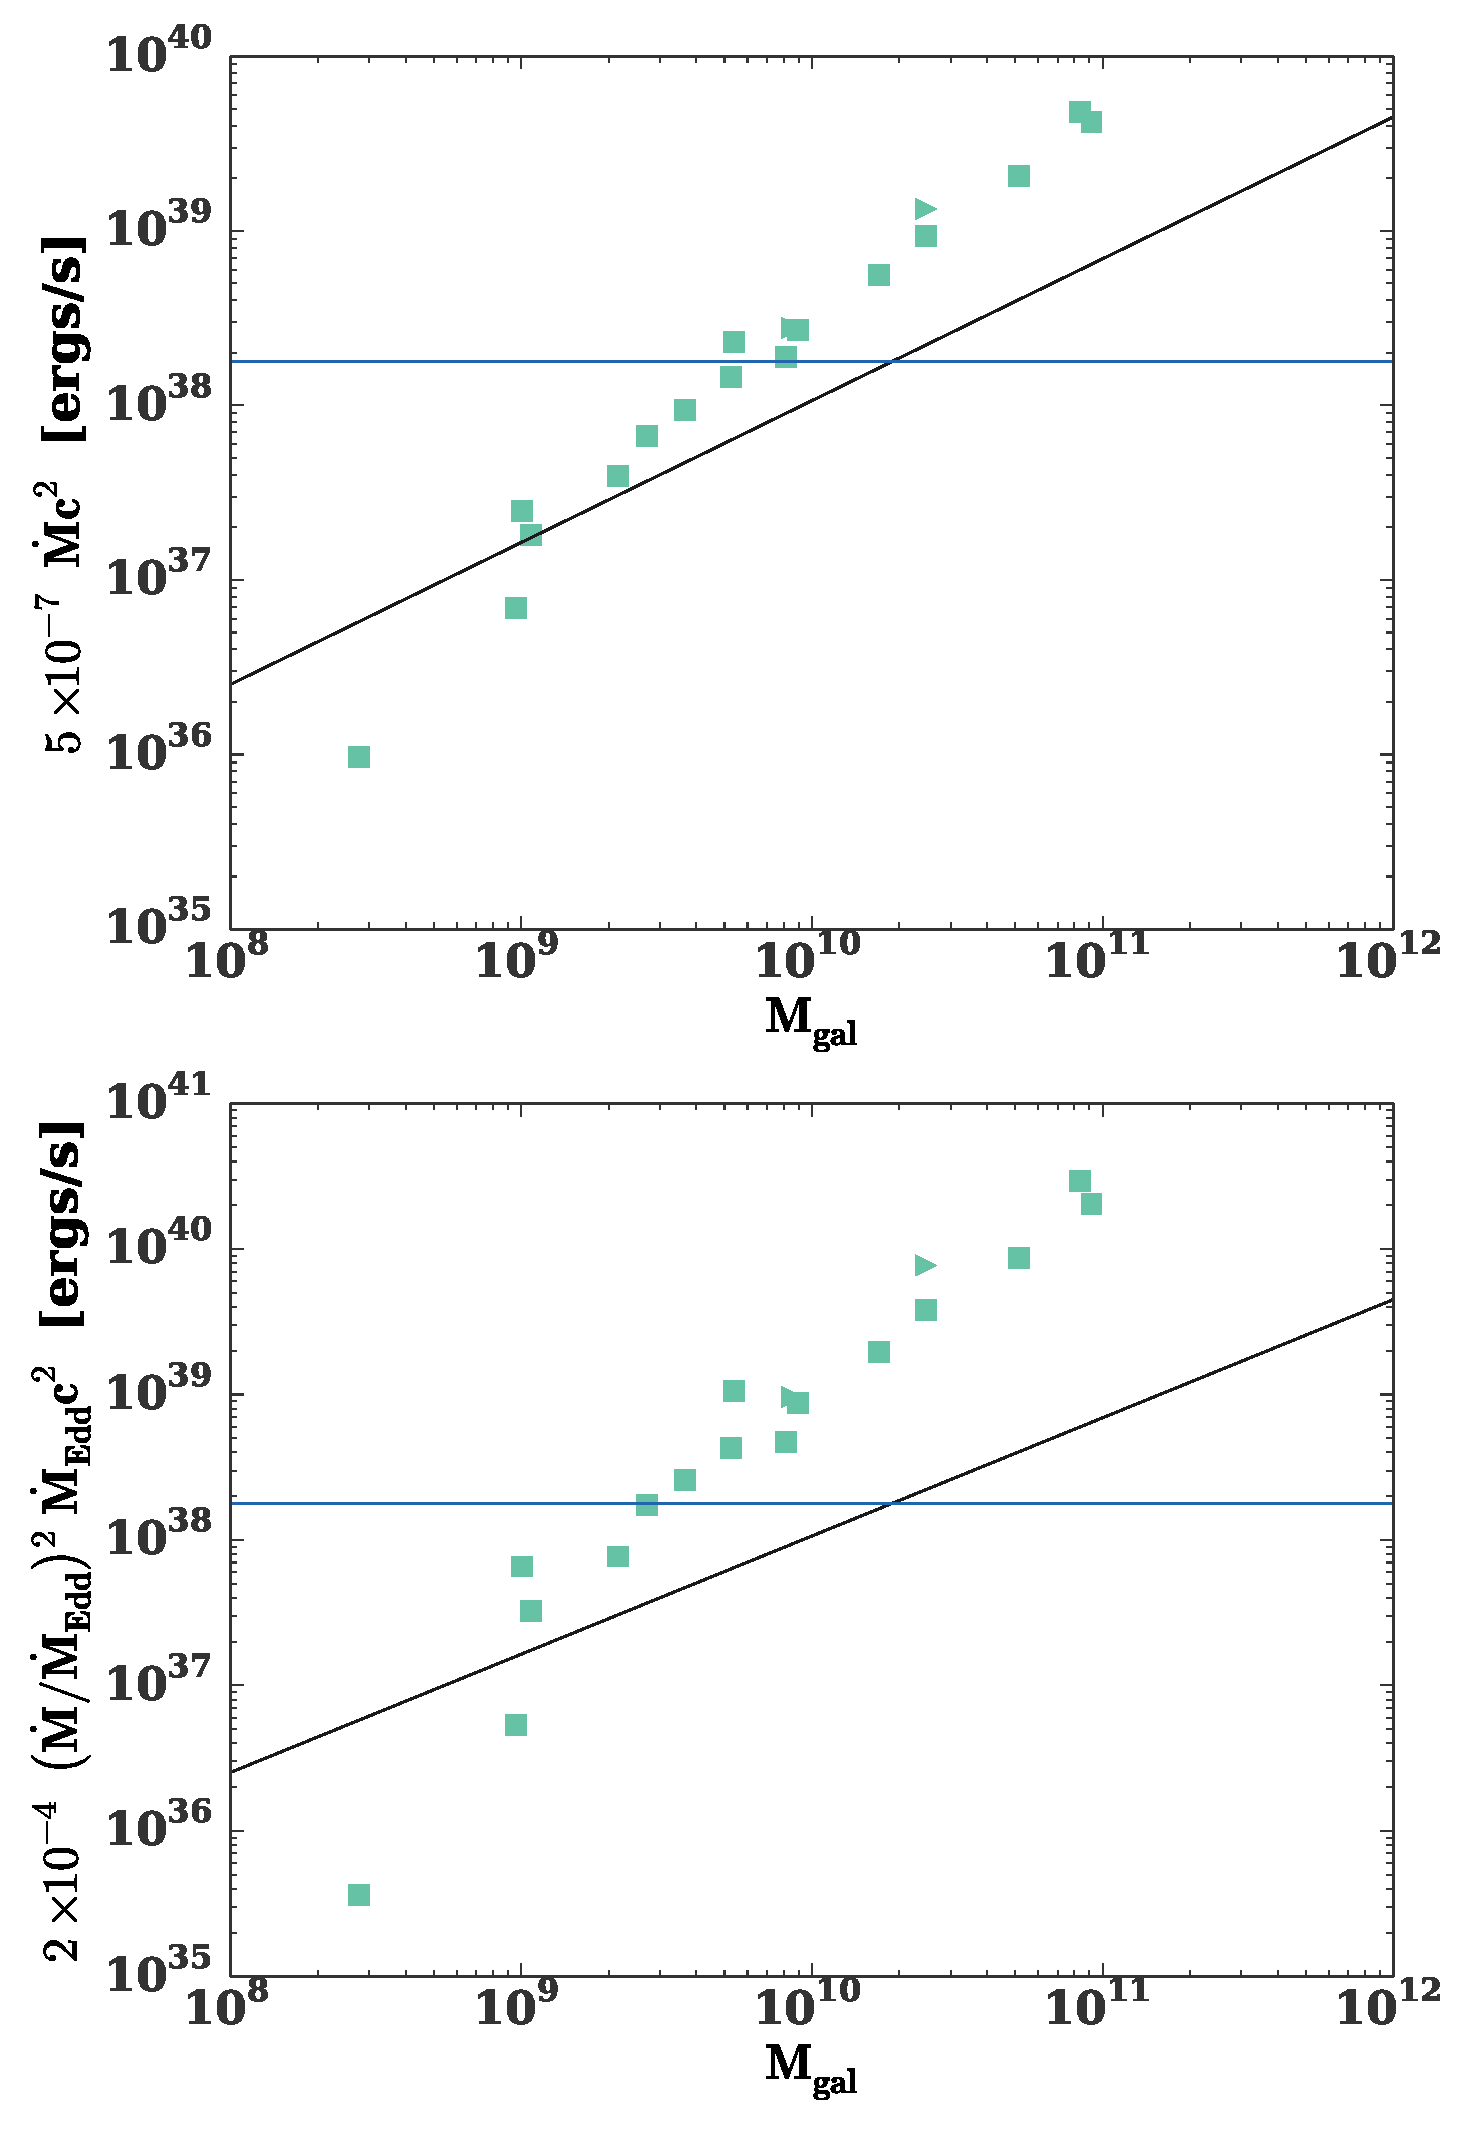
\includegraphics[width=\columnwidth]{bh_xray.eps}
% \caption{\label{fig:bh_xray} X-ray luminosity plotted as a function of
%   stellar mass for our solutions (points), the trend of nuclear x-ray
%   luminosity with stellar mass (black line) and the detection upper
%   limit (blue line) from Fig. 1 of \citealt{Miller+15}. In
%   the top panel we take the X-ray luminosity to be $\epsilon_1 \Mdot
%   c^2$, with $\epsilon_1=5\times 10^{-7}$ chosen to make our
%   luminosities comparable to those observed. In the bottom panel, we
%   take the accretion power to be quadratic in $\Mdot$. $L_x=\epsilon_2
%   \eddr \Mdot c^2$ with $\epsilon2$=$2\times10^{-4}$. For each galaxy
%   we choose the $\vwO=200$ km/s solution.  {\bf BDM: if possible, add actual x-ray data from Gallo+08!}}
% \end{figure}

\subsection{X-ray Diagnostics of SMBH Occupation}
\label{sec:occ}
The free-free emission from steady state gas flows in low mass
galactic nuclei may serve as useful diagnostics of the presence or
absence of a SMBH.  We focus primarily on low-mass galaxies in this
subsection, both because this is the portion of parameter space in
which gas inflow will generally proceed in a steady-state fashion, and
because of recent observations suggesting that a nontrivial fraction
of these galaxies may lack nuclear SMBHs.  If this absence is
confirmed, it could have implications for galaxy evolution, SMBH
recoil distributions, and SMBH seed formation models.

We can approximate the gas temperature as 

\begin{equation}
% T \approx \frac{\mu m_{\rm p} (\gamma-1)}{2\gamma k_{\rm B}}
% \left(\tilde{v}_{\rm w}^2 + GM_\bullet/r \right).
 \kb T \approx 2.1\times 10^{-25} \left(\tilde{v}_{\rm w}^2 + GM_\bullet/r
 \right) {\rm [cgs]}.
\end{equation}

In the absence of a central SMBH, we can expect to see an exponential
cutoff in the free-free X-ray spectrum at energies above

\begin{equation}
E_{\rm cut} = 0.32~{\rm keV} v_{500}^2,
\end{equation}

assuming $\gamma = 5/3$.  This cutoff will therefore be located in the
portion of the soft X-ray covered by {\it Chandra}'s ACIS
spectrometer.  By writing the free-free emissivity as

\begin{equation} 
\varepsilon_{\nu}^{\rm ff} = 6.8\times10^{-38}
\frac{\rm erg}{\rm s~cm^3~Hz} Z^2n_{\rm e}n_{\rm
i}T^{-1/2}\bar{g}_{\rm ff}\exp\left(\frac{-h\nu}{k_{\rm B}T}\right),
\end{equation}

where $Z$ is the atomic number of the ions, $n_{\rm e}$ and $n_{\rm
  i}$ are respectively the electron and ion number density, and
$\bar{g}_{\rm ff}$ is the Gaunt factor.  In the following we set
$n_{\rm e}=Y_{\rm e}n_{\rm i}$, and approximate
\begin{equation}
n_{\rm i} \approx \frac{\dot{M}}{(4\pi/3) \rs^2 \mu \mp}\sqrt{ \frac{r_{\rm s}}{ 2 G \Mbh} } \left( \frac{r}{\rs} \right)^{-n}.
\end{equation}

We now write the total spectral luminosity density seen in unresolved
X-ray observations above the cutoff energy as

\begin{align}
 L_{\nu}^{\rm ff} =& \int_0^{r_{\rm s}} 4\pi r^2 \varepsilon_{\nu}^{\rm ff}{\rm d}r \\
\approx & 2.8\times 10^{16} \, {\rm ergs \, s^{-1}
  \, Hz^{-1}} \left(\frac{\dot{M}}{10^{-5}M_\odot/{\rm
      year}} \right)^2 \left(\frac{\rs}{10^{-2}~{\rm pc}} \right)^{-1}
   \notag \\
& \times \left(\frac{h \nu}{0.5~{\rm keV}}\right)^{-3/2} \bar{Z}^2 \bar{g}_{\rm ff} Y_{\rm e} \notag \\
\approx & 3.9\times 10^{14} {\rm ergs~s^{-1}~Hz^{-1}}
\eta^2 \left(\frac{\Mbh}{10^{6}~{\Msun}} \right)^{1.96} \notag\\&\times
\left(\frac{h \nu}{0.5~{\rm keV}}\right)^{-3/2} v_{500}^{-2.8} \bar{Z}^2 \bar{g}_{\rm ff} Y_{\rm e} 
\end{align}

The second line of this equation makes the approximation that
$GM_\bullet/r$ dominates $\tilde{v}_{\rm w}^2$ throughout the
integrand, which will be true for energies modestly higher than
$E_{\rm cut}$.  The lower (upper) endpoint for this integral are
arbitrary so long as it is somewhat less (greater) than the radius at
which the observed frequency $\nu$ sees its exponential free-free
cutoff. We have also set $n=1$.

In general, these ``cut-off'' X-ray luminosities are quite small, and
even {\it Chandra} would have little hope of detecting them in any but
the nearest dwarf galaxies (e.g. the Magellanic clouds).  However, if
source confusion is not present, this technique could test for the
presence of IMBHs in very nearby dwarf galaxies, or more speculatively
Galactic star clusters.


\section{Discussion}
\label{sec:discussion}

\subsection{Demographics of SMBHs}

Our analytic expression for the accretion rate (eq.~[\ref{eq:mdot_analytic}]) can be translated into the growth time of the SMBH $t_{\rm grow} \equiv M_{\bullet}/\dot{M}$,
\begin{eqnarray}
  t_{\rm growth}/t_{\rm h} \approx 
  \begin{cases}
    250 M_{\bullet,8}^{-0.76}
    v_{500}^{3.8}   \eta_{0.02}  & \text{core} \\
    140 \Mbheight^{-0.48}
    v_{500}^{2.4}   \eta_{0.02}  & \text{cusp}, 
  \end{cases}
  \label{eq:tgrow_analytic}
\end{eqnarray}
which we have normalized in terms of the Hubble time.  

There is a maximum accretion rate for a thermally stable flow
(eqn. [\ref{eq:Mdotmax}]). This gives a lower bound on the growth
time from thermally stable accretion

\begin{align}
  t_{\rm growth}/t_{\rm h} \gsim
  \rm{max}\begin{cases}
    9 \eta_{0.02}^{-0.47} \Mbh^{-0.34} &, \text{core}\\
    15 \eta_{0.02}^{-0.59} \Mbh^{-0.29} &, \text{cusp}\\
    50  \eta_{0.02}^{-1} &, v_{\rm TI} < \sigma
  \end{cases}
  \label{eq:tgrow_min}
\end{align}

In Figure~\ref{fig:bh_growth} we plot the growth times for core and
cusp galaxies, with parameters chosen for the average star formation
history at each $\Mbh$ (see Figure~\ref{fig:vwSources}
and~\ref{fig:eta}). Core and cusp galaxies are shown in green and blue
respectively.  We also plot the maximum growth time for thermal
instability from equation~\eqref{eq:tgrow_min} in purple.

\begin{figure}
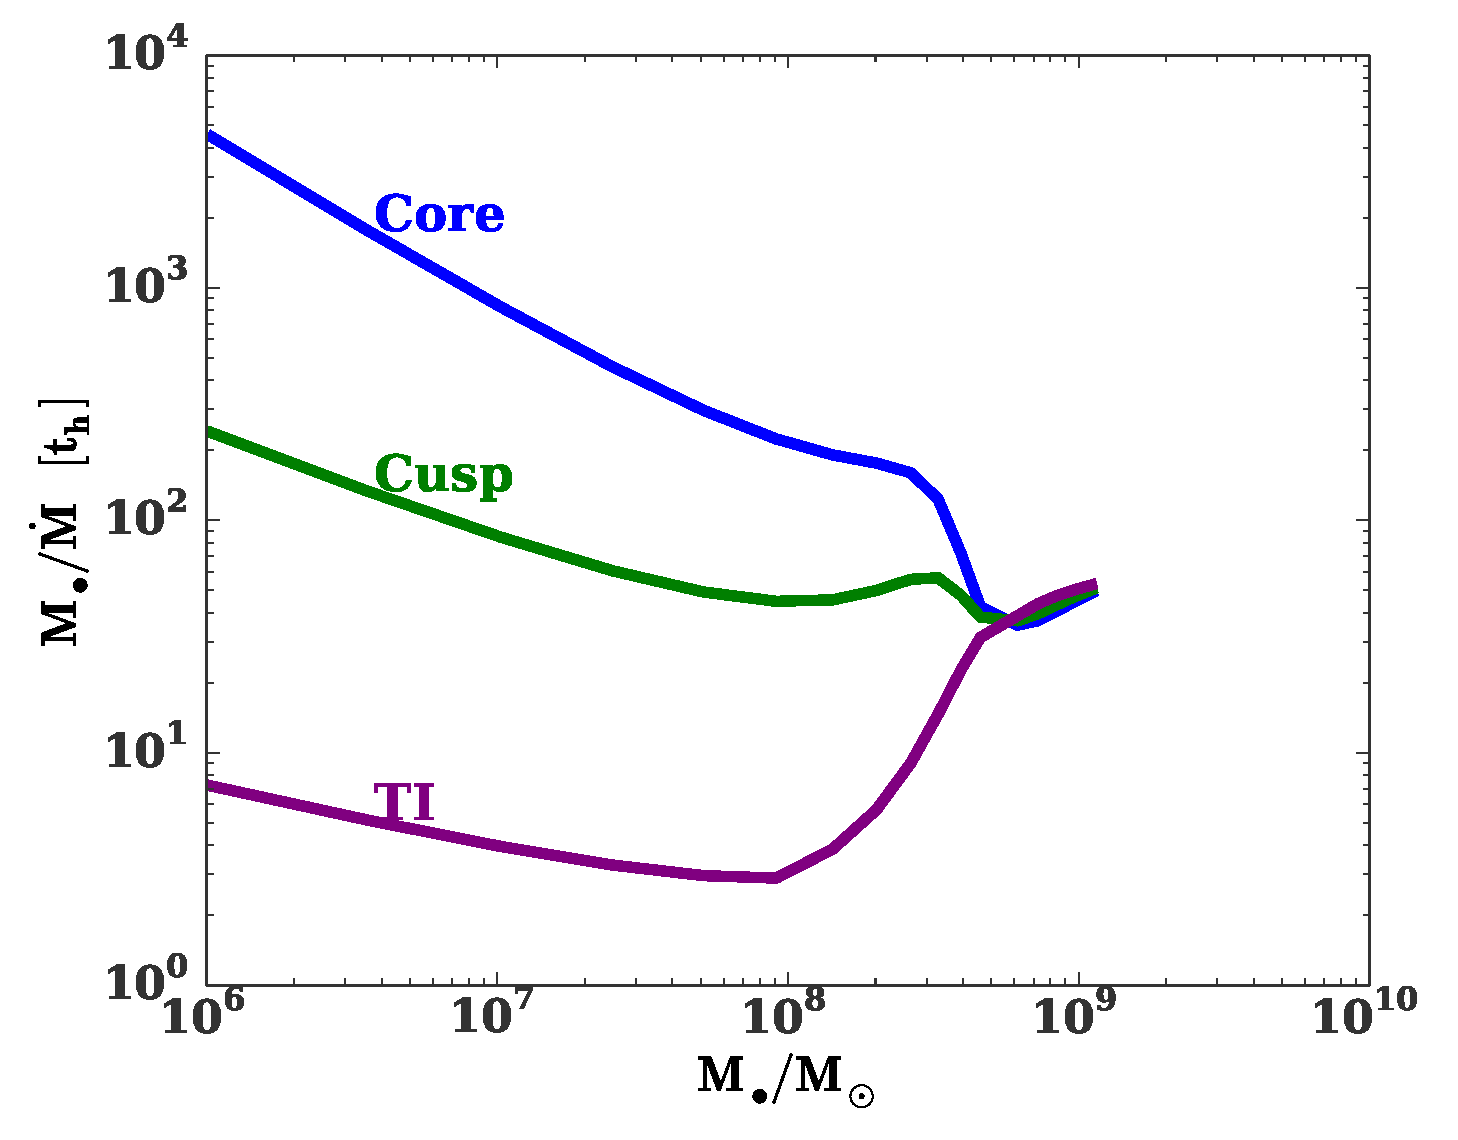
\includegraphics[width=\columnwidth]{bh_growth.eps}
\caption{\label{fig:bh_growth} Growth times $\Mdot/\MdotEdd$ in units
  of the Hubble time $\th$ for core ($\Gamma=0.1$, blue) and cusp
  ($\Gamma=0.8$, green). These are calculated from
  equation~\ref{eq:tgrow_analytic} with parameters chosen for the
  average star formation history at each $\Mbh$. We also plot a lower
  bound on growth time for a themally stable flow (purple) from
  equation~\eqref{eq:tgrow_min}.}
\end{figure}

\subsection{Cooling}
\label{sec:cooling}

\section{Discussion}

\begin{itemize}
\item{Fact that some low mass BHs appear to have nearly Eddington accretion rates, suggest an external origin - since the maximum Ia rate appears to be below this}
\item{Growth of low mass BHS, e.g. \citealt{Kauffmann&Heckman09}}
\end{itemize}

If cooling becomes important in the flow ($\tilde{v}_{w} < v_{\rm CI}$), it may lead to thermal instabilities.  There are two kinds of ``instabilities", global and local.  The global instability is simply that, if cooling becomes very rapid, the gas loses thermal pressure and starts to inflow faster, i.e. the entire CNM accretes.  In
practice this should could manifest as a large increase in the stagnation radius, due an effective {\it decrease} in the effective heating rate.  This global ``instability" is not a true instability insofar as the gas does not necessarily clump locally into low-T clouds.

However, \citet{McCourt+12} argue that even if cooling is exactly
balanced by heating everywhere, there is still a local thermal
instability that operates to turn hot gas into cold clouds.  However,
this local instability only causes a significant local drop-out of
mass from the hot medium (to low-T clouds), if the cooling timescale,
\begin{align}
\frac{\tcool}{\tff} &\equiv \frac{3\rho k T/2 \mu \mp}{\dot{q}_{\rm cool}} \approx \frac{9}{5} \left. \frac{q \vw^2/2}{\dot{q}_{\rm cool}}\right|_{\rs}
\end{align} 
is locally shorter than the approximately 10 times the free-fall
timescale $t_{\rm ff}$, where the last equality is evaluated at the
stagnation radius and makes use of equations~(\ref{eq:Tanalytic}) and
(\ref{eq:rhors2}).  We thus see that the condition $\tilde{v}_{w} \gtrsim v_{\rm
  crit}$ is also the condition for local instability, although the
prefactor may be slightly different.

\subsection{TDE Jets}

Plot showing final lorentz factor after the reverse shock crossing as a function of BH mass, using average star formation history.  place J1644+57 on the plot.

\subsection{Jet Feedback}

We also note
here that the kinetic heating rate is proportional to the SMBH mass to
a positive power, $v_{w}^{\bullet} \propto M_{\bullet}^{1(0.5)}$ for
core(cusp) galaxies, respectively. This dependence could have
important implications for the dependence of the average nuclear X-ray
luminosity of quiescent galaxies on the SMBH mass
($\S\ref{sec:mdot}$).

\subsection{Jet Power Correlation}

Accretion rates onto SMBHs can in principle be estimated directly by
assuming Bondi accretion and using high resolution X-ray observations
to estimate the gas temperature and density near the Bondi radius.
This technique has led to the intriguing conclusion that the Bondi
accretion power correlates with the AGN jet power (e.g.,
\citealt{AllenDunn+:2006a}; \citealt{Russell+13};
\citealt{FujitaKawakatu+:2014a}), the latter estimated from the energy
required to inflate the observed cavities within the X-ray emitting
gas.  In practice is it almost never possible to resolve the Bondi
radius, therefore requiring all such studies to extrapolate the
observed gas temperature and density profiles to smaller radial
scales.

\subsection{Nuclear Star Clusters}
Do nuclear star clusters in other galaxies look like scaled up/down
versions of the one in our own galaxy? If so this would imply a radial
gradient in the average of the stellar population which would imply a
heating which would be dependent on radius.

\subsection{SFR-AGN connection}
In fact it seems like the star formation rate may trace AGN
episodes. See e.g. http://arxiv.org/pdf/1501.07602.pdf. 

\subsection{Type II Supernovae}
Type II supernovae should provide some heating as well for younger
stellar populations...In fact at least on large scales they may be the
dominant source of heating on timescales of 10-40 Myr. 
  

  \section{Summary}
  \label{sec:summary}
  We have calculated steady-state models for circumnuclear medium of a
  sample of early type galaxies, assuming that gas is supplied
  entirely by stellar wind mass loss and heated by shocked stellar
  winds and SNe Ia. We may use these profiles to calculate an $\Mdot$
  onto each of sample galaxy's SMBH, and get the scaling of $\Mdot$
  with $\Mbh$. We may then compare our results with observed trends of
  nuclear x-ray luminosity. Our main conclusions may be summarized as
  follows.

  \begin{enumerate}
  %Younger population=>higher accretion rate; generally higher eta and
  %lower vw except for very young stellar populations.
  \item We find that $\eddr \propto \Mbh^{\alpha}$, where the value of
    $\alpha$ depends on the slope of the stellar density profile
    ($\alpha\simeq0.5,1$ for cusp and core galaxies respectively). One
    possible solution that the wind mass loss rate (i.e. $\eta$)
    increases with $\Mbh$, as would be expected if low mass SMBH
    preferentially hosted younger stellar populations. Another possible
    explanation is that the effective heating rate of the CNM $v_{w}$
    decreases with decreasing SMBH mass. This could again be due to an
    older stellar population, since $v_{w} \propto \eta^{−1/2}$
    for heating sources such as SN Ia and millisecond pulsars.
  \item We compare the $\Mdot$ for each of our solution to the one
    calculated from the Bondi formula. We find that they generally to
    a factor of a few. In our model the accretion rate is determined
    from the gas properties at the stagnation radius, $\rs$, which
    agrees with the Bondi radius, $\rb$, within a factor of a
    few. Thus, use of the Bondi formula is a good approximation.
  \item We compare our solutions for density and temperature to those
    inferred from Chandra x-ray observations by \citet{AllenDunn+:2006a}
    and \citet{RussellMcNamara+:2013a} for a handful of galaxies in
    which our sample overlap with theirs. In general, we cannot match
    the observed gas density slope on large scales. 
  \end{enumerate}
  
  \clearpage
  \appendix
  \section{Analytic Expression for the stagnation radius}
  \label{app:rs}
  
Here we derive an analytic expression for the steady-state stagnation radius $r_{\rm s}$.  The steady-state entropy equation (eq.~[\ref{eq:dsdt}]) can be manipulated to read
\begin{align}
T\dsdr=\frac{\Q}{\rho v} \label{eq:ss_entropy}
\end{align}
By definition, the velocity $v$ goes to zero at the stagnation radius.  In order to avoid the entropy derivate from diverging, the numerator of (\ref{eq:ss_entropy}) must also go to zero at $r_{\rm s}$, implying that
\begin{align}
 \frac{\gamma}{\gamma-1} \frac{p|_{\rs}}{\rho|_{\rs}}=\frac{\vw^{2}|_{\rs}}{2} \Rightarrow \frac{\kb T|_{\rs}}{\mu \mp}=\gammafi \frac{\vw^{2}|_{\rs}}{2} .
\label{eq:appTanalytic}
\end{align}
Combining (\ref{eq:ss_entropy}) with the first law of thermodynamics,
\begin{align}
T\dsdr =& \frac{1}{\gamma-1}\ddr{(p/\rho)}-\frac{p}{\rho^2}\ddr{\rho} = \\
& 
\frac{1}{\gamma-1}\left.\ddr{(p/\rho)}\right|_{\rs}+\frac{\densSlope}{\rs}  \frac{p|_{\rs}}{\rho|_{\rs}}=\left.\underbrace{\frac{\Q}{\rho  v}}_{A}\right|_{\rs}, 
% \label{eq:first_law}
\end{align}
where $\densSlope\equiv -\left.d\log(\rho)/d\log(r)\right|_{\rs}$.  The term on the right can be evaluated using L'Hopital's rule, yielding
%\begin{align}
 % &\lim_{r \rightarrow \rs} A=\frac{\lim_{r \rightarrow \rs}
  %  \frac{d}{dr}\left[q (r)\left(\ke -\gammaf
   %     \frac{p}{\rho}+\kew\right)\right]}{\lim_{r \rightarrow \rs}
    %\frac{d}{dr} \left(\rho v\right)}\\
  %&=\frac{ q'|_{\rs} \overbrace{\left.\left(\ke
   %     -\gammaf\frac{p}{\rho}+\kew\right)\right|_{\rs}}^0+ q|_{\rs}
    %\frac{d}{dr} \left[\left(\ke -\gammaf
     %   \frac{p}{\rho}+\kew\right)\right]_{\rs}}{\underbrace{\rho'|_{\rs}
      %v|_{\rs}}_0 +\underbrace{v'|_{\rs}\rho|_{\rs}}_{q|_{\rs}}}\\
\begin{align}
  \lim_{r \rightarrow \rs} A = \frac{d}{dr} \left[\left(\ke -\gammaf \frac{p}{\rho}+\kew\right)\right]_{\rs}
\end{align}
Now using the definition $\vw^2=\vwO^2+ G \Menc/r$, where
$\Menc=\Mbh+\Mstar$, and assuming $\Mstar \sim r^{2-\Gamma}$, we find that
\begin{align}
\lim_{r \rightarrow \rs} A=-\gammaf
\left.\ddr{(p/\rho)}\right|_{\rs}-\frac{G \Menc|_{\rs}}{2 \rs^2}+(2-\Gamma) \frac{G
  \Mstar|_{\rs}}{2 \rs^2}.
\end{align}
Substituting this expression back into equation (\ref{eq:first_law}) and using equation (\ref{eq:appTanalytic}) gives
\begin{align}
&\frac{\gamma+1}{\gamma-1}
\left.\ddr{(p/\rho)}\right|_{\rs}+ \frac{\gamma-1}{\gamma} \frac{\densSlope}{\rs} \vw|_{\rs}^{2} = (2-\Gamma) \frac{G
  \Mstar|_{\rs}}{2 \rs^2} -\frac{G \Menc|_{\rs}}{2 \rs^2}.  \label{eq:rs1}
\end{align}
A second equation results from evaluating the momentum equation (eq.~[\ref{eq:dvdt}]) at the stagnation point
\begin{align}
&\frac{1}{\rho}\dpdr=- \frac{G\Menc}{\rs^2} \Rightarrow
&\ddr{(p/\rho)}+\frac{p}{\rho}
\underbrace{\frac{d\log(\rho)}{dr}}_{-\densSlope/r} = -\frac{G \Menc}{\rs^2} \label{eq:HSE}
\end{align}
Finally, combining equations (\ref{eq:rs1}) and (\ref{eq:HSE}) gives 

\begin{align}
\rs=\frac{G \Mbh}{\densSlope \vw^{2}|_{\rs}}\left(\frac{9-\Gamma}{2}
  \frac{M_{\star}|_{\rs}}{\Mbh} +\frac{7}{2}\right),
\end{align}
where we have assumed $\gamma=5/3$.

In terms of just the additional wind heating parameter, $v_w$,

\begin{align}
\rs=\frac{G \Mbh}{\densSlope v_w^{2}|_{\rs}}\left[\left(\frac{9-\Gamma}{2} -\densSlope\right) \frac{\Mstar|_{\rs}}{\Mbh} +\frac{7}{2}-\densSlope\right].
\label{eq:rs2main}
\end{align}


Defining $\eta \equiv \vwO/\sigma_{\rm soi}$, this relationship can be
reparameterized as follows:
\begin{align}
  \frac{\rs}{\rsoi}=\frac{1}{2 \zeta^2 \densSlope}\left[
    \frac{\Mstar|_{\rs}}{\Mbh}\left(\frac{9-\Gamma}{2}-\densSlope\right)+\left(\frac{7}{2}-\densSlope\right)\right]
\end{align}

%{\bf AG: Note that I have taken sigmainf=2 G Mbh/rinf. Commented out
%equations have sigmainf=G Mbh/rinf}. 
For cusp galaxies ($\Gamma\simeq1$) we have $\Mstar|_{\rs}/\Mbh=x$, $A=4$, and $B=7/2$ for $\gamma = 5/3$, such that 
\begin{align}
\x=\frac{7-2\densSlope}{4\zeta^2 \densSlope+2\densSlope-8}
%\x=\frac{7-2\densSlope}{2\zeta^2 \densSlope+2\densSlope-8}
\end{align}
In the limit of zero wind heating $\eta \rightarrow 0$, no solution
for $r_{\rm s}$ exists unless the gas density profile at the
stagnation radius is steep, 3.5 $<\densSlope<$ 4.

For core galaxies ($\Gamma \simeq 0$) with $\Mstar/\Mbh=x^2$, A=9/2,
and B=7/2, the stagnation radius instead obeys a quadratic equation
\begin{align}
\x=\frac{\zeta^2 \densSlope \pm \sqrt{\zeta^4 \densSlope^2 - \left(\frac{9}{2}-\densSlope\right)
    \left(\frac{7}{2}-\densSlope\right)}}{\left(\frac{9}{2}-\densSlope\right)}
%\x=\frac{\zeta^2 \densSlope \pm \sqrt{\zeta^4 \densSlope^2 - 4 \left(\frac{9}{2}-\densSlope\right)
%\left(\frac{7}{2}-\densSlope\right)}}{2 \left(\frac{9}{2}-\densSlope\right)}
\label{eq:rstag}
\end{align}
In this case no solution exists in the zero heating limit ($\zeta
\rightarrow 0$) unless $3.5<\densSlope<4.5$.

When $\Mstar << \Mbh$ at the stagnation radius, the relationship
between $\rs$ and $\vw$ is greatly simplified.
\begin{align}
\rs=\frac{7}{2}\frac{G \Mbh}{\densSlope \vw^2},
\end{align}
where the pre-factor on the right-hand side corresponds to
$\gamma=5/3$ and $\Gamma=1$ or 0.  



%%% Local Variables:
%%% mode: latex
%%% TeX-master: "ms"
%%% Ennd:



\section{Analytic model for dependence of wind heating $\vwO^{\star}$ on stellar age}
\label{app:windheat}
% If we assume that a stellar population forms
% impulsively in the distant pass with IMF $\mu(m_*)$(with minimum mass
% $m_0$ and maximum mass $m_1$), then the surviving mass fraction at any
% future time $t$ is given by
% \begin{equation}
% f(t) =\frac{ \int_{m_0}^{m_{\rm T}(t)} m_* \mu(m_*) dm_* }{ \int_{m_0}^{m_1} m_* \mu(m_*) dm_* },
% \end{equation}
% where the main sequence turnoff mass is approximately
% \begin{equation}
% m_{\rm T}(t) \approx 2.5M_\odot~ \left( \frac{t}{10^9~{\rm yr}} \right)^{-0.4}.
% \end{equation}
% For a Salpeter IMF $\mu(m_*) \propto m_*^{-2.35}$ with $m_0=0.1M_\odot$ and $m_1=100M_\odot$,
% \begin{equation}
% f_{\rm Sal}(t) = 1.098 - 0.490 \left(\frac{t}{10^{10}~{\rm yr}} \right)^{0.14}
% \end{equation}
% {\bf NCS: we should probably use a Kroupa/Chabrier IMF, but this gets the ball rolling.}
% If we approximate post-main sequence evolution as instantaneous and define $\lambda(\Mstar)$ as the fractional mass lost during all stages of stellar evolution, then the mass loss rate density
% \begin{equation}
% q(t) = \frac{\rho_*}{\bar{m}_*} \lambda(m_{\rm T}(t)) m_{\rm T}(t) \frac{df}{dt},
% \end{equation}
% where the mean stellar mass $\bar{m}_* = \int_{m_0}^{m_{\rm T}(t)} \Mstar\mu(\Mstar)d\Mstar \approx 0.3 M_\odot$.  Further approximating $\lambda(\Mstar)=0.5$, and using the Salpeter IMF once more, gives
% \begin{equation}
% q(t) = \frac{\rho_*}{10^{10}~{\rm yr}} \times 0.11 \left(\frac{t}{10^{10}~{\rm yr}} \right)^{-1.26}.
% \end{equation}
% This is a specific, time-dependent definition of $\eta(t) (=0.11(t/t_{\rm h})^{-1.26})$; if we consider different star formation scenarios (for example, continuous star formation) or different IMFs, it will change.  Once these free parameters are specified, however, we can answer an important question: do young stellar populations increase or decrease the SMBH feeding rate $\dot{M}$?  Clearly, $\eta(t)$ is larger for young stellar populations, but these stars also have high wind velocities that diminish the stagnation radius.  Crudely approximating $v_{\rm w}=75~{\rm km~s}^{-1}$ for $m_{\rm T} < 10M_{\odot}$ and $v_{\rm w}=3000~{\rm km~s}^{-1}$ for $m_{\rm T} > 10M_{\odot}$ (motivated by the transition from dust-driven wind loss on the AGB to line-driven wind loss from Wolf-Rayet stars), we can employ the relation $\dot{M} \propto \eta(t) r_{\rm s}^{2-\Gamma}\propto \eta(t) v_{\rm w}^{-4+2\Gamma}$ (where $\rho_* \propto r^{-\Gamma}$) to determine the impact of stellar ``youth'' on SMBH feeding rates.
% {\bf AG:As I previously mentioned this discussion of the eta is not
%   quite correct...}
% \begin{figure}
% 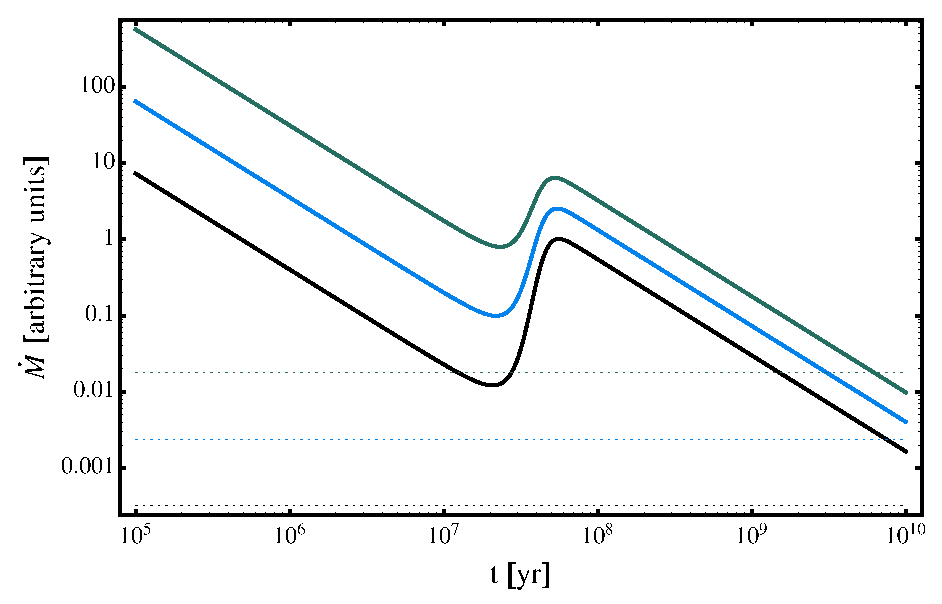
\includegraphics[width=\columnwidth]{NickPlot.eps}
% \caption{\label{NickPlot} SMBH feeding rates $\dot{M}=\eta(t) \times \Mstar(r_{\rm s})$, in arbitrary units.  The green, blue, and black curves are for galaxies with $\Gamma$ values of $0.1$, $0.5$, and $0.9$, respectively.  Solid curves represent impulsive-mode star formation, while dotted curves represent continuous-mode star formation. {\bf NCS: I think these old continuous curves are wrong, need to revise}}
% \end{figure}

% In Fig. \ref{NickPlot} we plot $\dot{M}$, in arbitrary units, as a
% function of time, for three different stellar density profiles $\Gamma
% = \{1.1, 1.5, 1.9\}$ (which are normalized to have the same mass at an
% influence radius $r _{\rm soi}=10~{\rm pc}$ around a $10^7M_\odot$
% SMBH).  We parametrize the wind velocity as
% \begin{equation} \frac{v_{\rm w}}{3000 ~\rm
% km~s^{-1}}=520-495\tanh\left( \frac{t-10^{7.5}~{\rm yr}}{10^{7}~{\rm
% yr}}\right). \label{NickV1}
% \end{equation} This counts Type II SNe heating as ``winds;'' if
% instead we are in the portion of parameter space where $r_{\rm II}$ is
% very large, then we use the alternate parametrization
% \begin{equation} \frac{v_{\rm w}}{3000 ~\rm
% km~s^{-1}}=520-495\tanh\left( \frac{t-10^{7}~{\rm yr}}{10^{6.5}~{\rm
% yr}}\right), \label{NickV2}
% \end{equation} which only allows short lived Wolf-Rayet stars to
% contribute to the high-heating mode.  The ``impulsive burst'' mode of
% star formation produces large ($\sim 10$) differences between the
% three $\dot{M}$ curves at early times, when $r_{\rm s}$ is small, but
% smaller ($\sim 3$) differences at late times, when $r_{\rm s}$ is
% large.  We also plot, as dotted curves, a simple model for the
% ``continuous'' mode of star formation, where mass loss is calculated
% as $\bar{\eta} = \int\eta(t)dt/t_{\rm h} \approx 4$ and an average
% energy injection in the wind is calculated as $\bar{v_{\rm
% w}^2}=\int\eta(t)v_{\rm w}^2(t)dt/\bar{\eta} \approx (800~{\rm
% km~s}^{-1})^2$.  Interestingly, the continuous mode of star formation
% produces small differences from late-time $\dot{M}$ seen in cusp
% galaxies with impulsive star formation; however, continuous mode star
% formation decreases late-time $\dot{M}$ by an order of magnitude
% relative to impulsive star formation in core galaxies.  {\bf NCS: I
% think this old discussion of MDot in the continuous limit is wrong,
% need to revise}

The energy and mass injection from stellar winds will be the sum ofthe
contributions from main sequence and post-main sequence (PMS) stars.
For an impulsively formed stellar population of age $t$, the mass
injection rate per unit stellar mass,$\dot{\bar{m}}(t)$, and  the energy
injection rate per unit stellar mass, $\dot{\bar{e}}(t)$,  will be given by

\begin{align} 
  \dot{\bar{m}}(t) &= \frac{\Delta M(t) \mu(M_{\rm TO}(t))
    \left|\dot{M}_{\rm TO}(t)\right| + f_{\rm MS} \int_{m_0}^{m_{\rm
        T}(t)}
    \dot{m}(\Mstar, t) \mu(\Mstar) {\rm d}\Mstar }{\bar{m}_*}\\
  \dot{\bar{e}}(t) &=\dot{e}_{\rm TO}(t)+ f_{\rm MS} \int_{m_0}^{m_{\rm T}(t)}
  \frac{\vw^2(\Mstar, t) \dot{m}(\Mstar, t) \mu(\Mstar) {\rm d}\Mstar}{\bar{m}_*}.
  \label{eq:edotImp}
\end{align} 

The first terms in each expression above correspond to the
contributions from PMS stars, while the second terms correspond to the
contributions from main sequence stars. The main sequence winds are a
small fraction of the mass, and they may be not be thermalized and
mixed with the rest of the injected gas. Thus, we include a
thermalization efficiency, $ 0\le f_{\rm MS}\le 1$, in
equation~\eqref{eq:edotImp}. Throughout this paper we set $f_{\rm
  MS}=1$. 

We assume a Salpeter IMF $\mu(\Mstar)\sim M^{-2.35}$, truncated at $0.1
\Msun$ on the low mass end and at $100 \Msun$ on the high mass
end. The corresponding mean stellar mass, $\bar{m}_*$ is 0.35 $\Msun$.

For the turnoff mass, $M_{\rm TO}$, we take the following fitting
formula 

\begin{align}
\log(M_{\rm TO})=0.24 + 0.068 x^2-0.34 x+4.76 e^{-4.58 x},
\end{align}

where $x=\log(t/10^9 {\rm years})$ and $M_{\rm TO}$ is in units
$\Msun$. This fit is designed to reproduce the results in 
Table 9 of \citet{MaederMeynet:1987a} and then asymptotes to the fit
for $M_{\rm TO}$ given in equation (9) of \citet{CiottiOstriker:2007a}
for intermediate and late times ($t \gsim 10^8$ years).

For $\Delta M(t)$ we use equation (10) from \citet{CiottiOstriker:2007a}

\begin{align}
\Delta M=
\begin{cases}
0.945 M_{\rm TO}-0.503 & M_{\rm TO} < 9 \Msun\\
 M_{\rm TO}-1.4 \Msun &  M_{\rm TO} \ge 9 \Msun
\end{cases}
\end{align}

To estimate the mass loss from main sequence stars
$\dot{m}(\Mstar, t)$,
we use equation 4 \citet{SchroderCuntz:2005a}\footnote{This
  prescription is a generalization of the Reimers' mass loss law. This
expression is derived assuming the stellar wind results from the
turbulent overflow of moaterial in the chromosphere or underneath it.} {\bf AG:
  unfortunately this is not really meant for MS stars...}

\begin{align}
  \dot{m}(\Mstar)=8 \times 10^{-14} \frac{L_* R_*}{\Mstar}
  \left(\frac{T_{\rm eff}}{\rm 4000 K}\right)^{3.5}
  \left(1+\frac{g_{\odot}}{4300 g_*}\right) \Msun \pyear,\
\end{align}

where  $R_*$, $L_*$, $T_{\rm eff}$ and $g_*$ are the stellar radius,
luminosity, effective and surface gravity respectively. $g_{\odot}$ is
the stellar surface gravity. To calculate $R_*$ and $L_*$ we use the
following scaling relations (taken from Kippenhann and Weygert Figures
22.2 and 22.3).

\begin{align}
L_*=
\begin{cases}
L_{\odot} (\Mstar/\Msun)^{3.2} & \Mstar > \Msun \\
L_{\odot} (\Mstar/\Msun)^{2.5} & \Mstar \le \Msun
\end{cases}
\end{align}

\begin{align}
r_*=
\begin{cases}
R_{\odot} (\Mstar/\Msun)^{0.57} & \Mstar > \Msun \\
R_{\odot} (\Mstar/\Msun)^{0.8} & \Mstar \le \Msun
\end{cases}
\end{align}


To get a handle on $\dot{e}_{\rm TO}(t)$, we use the results from
\citet{VossDiehl+:2009a} who use a population synthesis code to
simulate the mass and energy injection into the ISM from an OB
association. For the first $\sim 10$ Myr the energy injection will
come from energetic Wolf-Rayet star winds. The energy injection rate
per massive star ($\Mstar>8 \Msun$), $\dot{\mathcal{E}} (t)$, from
stellar winds is plotted in the top panel of their Figure 7 and is
well fit {\bf AG: A little more detail here...} by

\begin{align}
\dot{\mathcal{E}} (t)=
\begin{cases}
  1.3 \times 10^{36} {\rm ergs/s} & t<4 \times 10^6 {\rm years}\\
  1.3  \times 10^{36} {\rm ergs/s} \left(\frac{t}{4 \times  10^6}\right)^{-3.73} & t \ge 4 \times 10^6 {\rm years}.
\end{cases}
\label{eq:voss}
\end{align}

 $\dot{e}_{\rm TO}(t)$ is related to $\dot{\mathcal{E}}$  via 

\begin{align}
\dot{e}_{\rm TO}(t)=f_{8} \dot{\mathcal{E}} / \bar{m}_*,
\label{eq:eto}
\end{align}

where $f_{8}$ is the fraction of the stellar population with
$\Mstar>8 \Msun$. $f_8=2.6 \times 10^{-3}$ for our assumed Salpeter
IMF.  Equation~\eqref{eq:voss} and~\eqref{eq:eto} will be valid onlyfor $t
\lsim 10$ Myr. However, the turnoff contribution will become extremely
energetically subdominant at later times as far slower dust-driven
winds come to dominate the energy budget {\bf AG: Nick check--is the
  preceding sentence accurate}

We calculate the wind velocity for main sequence winds $v_w (\Mstar,
t)$ using...{\bf AG:Current just use the value for the sun~430 km/s
  replace with the real prescription we end up using.}

The effective wind velocity in the impulsive limit may then be written
as 

\begin{align}
\bar{v}_w(t)=2 \dot{\bar{e}}(t)/\dot{\bar{m}}(t)
\label{eq:vwImp}
\end{align}

We plot $\bar{v}_w$ in Figure~\ref{fig:vwImp}.

\begin{figure}
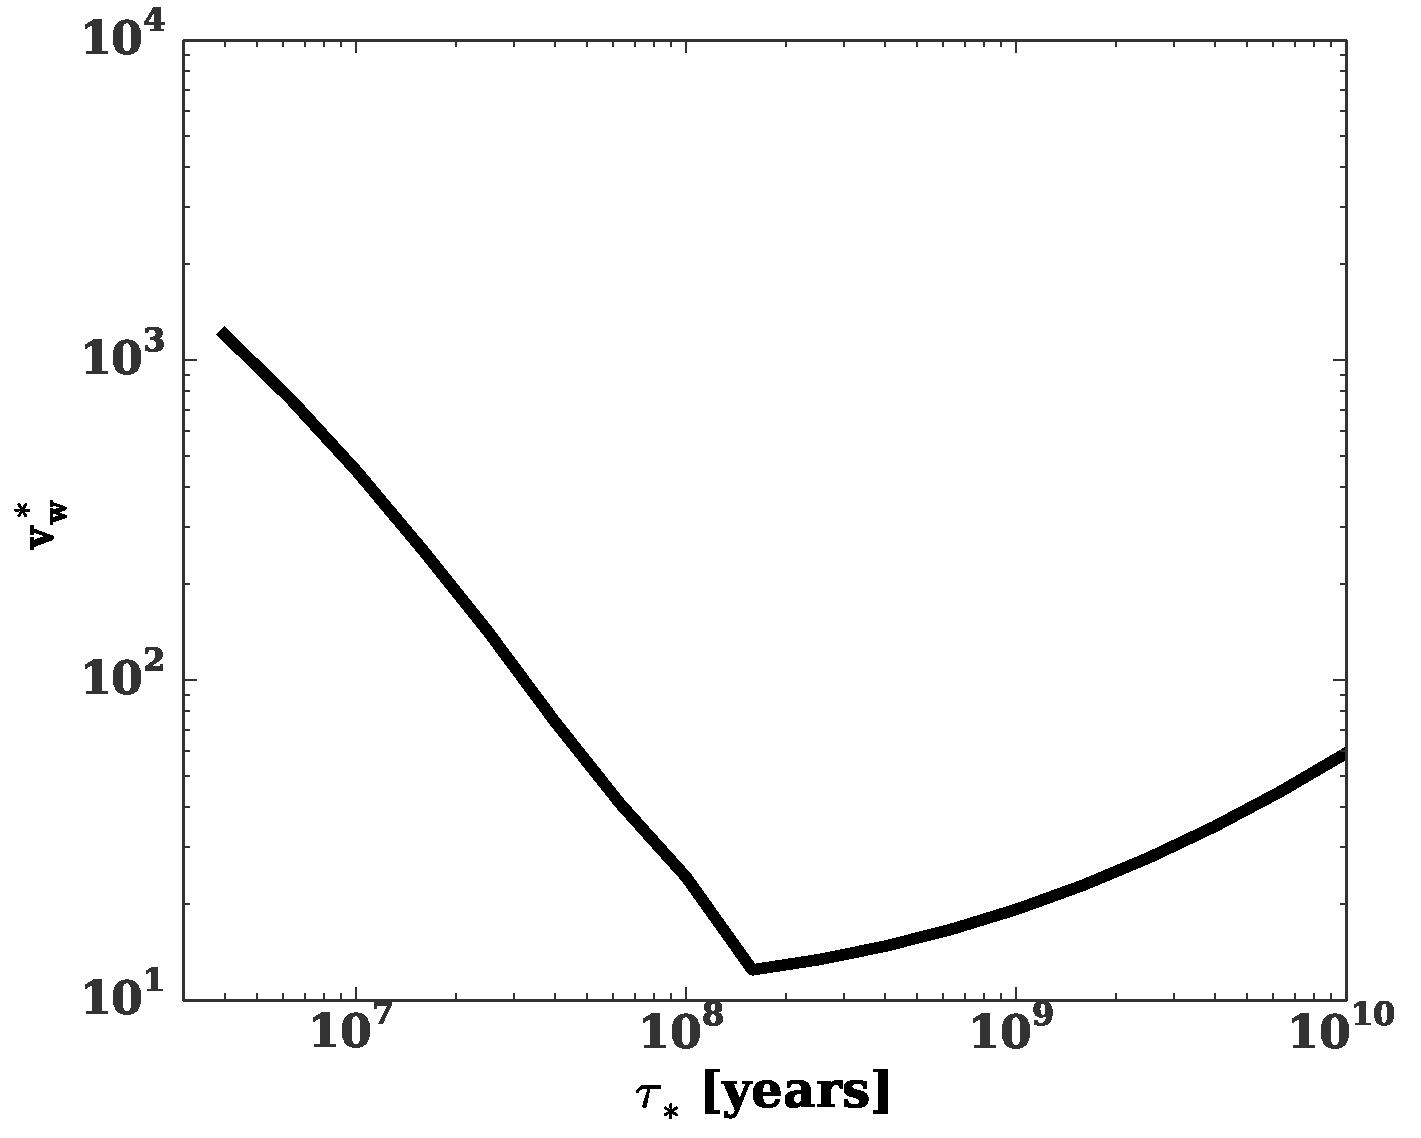
\includegraphics[width=\columnwidth]{vwImp.pdf}
\caption{\label{fig:vwImp} The effective $\vw$ from stellar winds from
  a stellar population formed in a starburst $t$ years ago.}
\end{figure}

We can then use these integrated quantities to determine the effective
$V_w$ for arbitrary star formation histories. For a stellar population
with star formation rate $S(t)$ 

\begin{align} 
  \dot{M}(t) &= \int_0^t S(t_1) \dot{\bar{m}}(t-t_1){\rm
      d}t_1\\
  \dot{E}(t) &= \int_0^t S(t_1) \dot{\bar{e}}(t-t_1){\rm
      d}t_1\\
  V_w^2(t) &=2 \dot{E}(t)/\dot{M}(t)
\end{align}

\begin{figure}
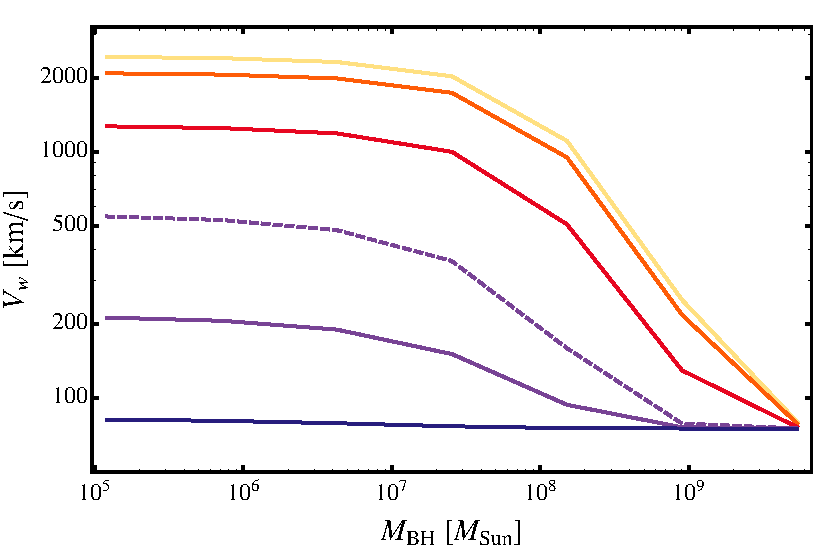
\includegraphics[width=\columnwidth]{vw.pdf}
\caption{\label{NickPlot2} Effective wind velocities $V_{\rm w}$ for
different $S(t)$.  The yellow and orange curves are the Moster SF
histories, with and without Type II SNe, respectively.  The red,
purple, and blue curves are Moster SFs convolved with a $\sin^2(t)$
function normalized to $10^7$, $10^8$, and $10^9$ yr fluctuations,
respectively.  These solid curves lack SN, but the dashed purple curve
possesses it.  Effective $V_{\rm w}$ is strongly diminished when the
variability timescale is greater than $\sim$ twice the duration of
high-velocity winds.}
\end{figure}

We show $V_{\rm W}$ for different star formation histories in
Fig. \ref{NickPlot2}.  In particular, we use Eqs. 17-20 from Moster et
al and the $M_{\rm BH}-M_{\rm halo}$ relation from Bandara et al {\bf
(NCS: add real refs)} to define $S(t)$ for particular galaxies.  It
seems that ``bumpy'' SF histories severely diminish $V_{\rm w}$ if the
timescale for SF variability is a factor of a few or more greater than
the duration of high-velocity winds (either 10 or 40 Myr).

%%% Local Variables: 
%%% mode: latex
%%% TeX-master: "ms"
%%% End: 


  \footnotesize{
    \bibliographystyle{mn2e}
    \bibliography{master}
  }
\end{document}
